
\documentclass{sig-alternate-2013}
\pdfpagewidth=8.5in
\pdfpageheight=11in
\newfont{\mycrnotice}{ptmr8t at 7pt}
\newfont{\myconfname}{ptmri8t at 7pt}
\let\crnotice\mycrnotice%
\let\confname\myconfname%

\permission{Permission to make digital or hard copies of all or part of this work for personal or classroom use is granted without fee provided that copies are not made or distributed for profit or commercial advantage and that copies bear this notice and the full citation on the first page. Copyrights for components of this work owned by others than the author(s) must be honored. Abstracting with credit is permitted. To copy otherwise, or republish, to post on servers or to redistribute to lists, requires prior specific permission and/or a fee. Request permissions from permissions@acm.org.}
\conferenceinfo{SIGCOMM'14,}{August 17--22, 2014, Chicago, IL, USA. \\
{\mycrnotice{Copyright is held by the owner/author(s). Publication rights licensed to ACM.}}}
\copyrightetc{ACM \the\acmcopyr}
\crdata{978-1-4503-2836-4/14/08\ ...\$15.00.\\
http://dx.doi.org/10.1145/2619239.2626331}

\clubpenalty=10000 
\widowpenalty = 10000



%\documentclass[letterpaper,twocolumn,10pt]{article}
%\usepackage{usenix,epsfig,endnotes}

%\thispagestyle{empty}

\usepackage{subfigure, verbatim, soul, comment, pifont, array, url, amsmath, multirow, latexsym, tabularx}
\usepackage{ifpdf, rotating, colortbl, graphicx}
%\usepackage[boxed]{algorithm}
\usepackage{algorithm, wrapfig, algorithmic, xspace, url, bbm, wrapfig, sidecap}
%\usepackage{wrapfig, xspace, url, wrapfig, sidecap}

\newcommand{\auspice}{Auspice}

\newcommand{\uniform}{Random}
%\newcommand{\kmedoids}{K-Mediods}
%\newcommand{\locaware}{Locality}
%\newcommand{\opt}{Optimal}
\newcommand{\optimal}{Optimal}
\newcommand{\beehive}{DHT+Popularity}
\newcommand{\codons}{DHT+Popularity}
\newcommand{\staticthree}{Random-M}
\newcommand{\static}[1]{Random-#1}
\newcommand{\replicateall}{Replicate-All}

\newcommand{\tbd}[1]{\textcolor{red}{\bf{[TBD:} #1]}}
\newcommand{\tbdf}[1]{\footnote{\bf{TBD:}#1}}
\newcommand{\eat}[1]{}
\newcommand{\para}[2]{{\bf{[#1]}}\\#2}
\newcommand{\blue}[1]{#1}
%\newcommand{\blue}[1]{\textcolor{blue}{#1}}
\newcommand{\rmCR}[1]{}


\newcommand{\msocket}{msocket}

\newcommand{\vsp}{\vspace{-0.06in}}
\newcommand{\figvsp}{\vspace{-0.2in}}

\newcommand{\asymb}{*}

\begin{document}
\title{Demand-aware geo-distributed placement for low latency}


\maketitle

%%!TEX root = New.tex
\begin{abstract}

Many datacenters are primarily used for content delivery. These datacenters are typically lightly loaded during normal operation, and hence have significant potential for saving energy. However, saving energy by shutting off servers could reduce cache-hit rates and by shutting off network components could increase datacenter network congestion; both events hurt user-experience. Due to these perceived risks, operators leave entire datacenters in an always on state foregoing all energy savings.

Towards the goal of saving energy in data center networks, we present \shrink, a cluster manager that makes power management decisions for networks and servers in a coordinated manner  to maximize energy savings, and  decides load balancing and traffic engineering  to ensure a minimal impact on user-perceived performance.
Further, \shrink\ orchestrates content transfers before server shutdown events to minimize the impact of server shutdown on cache hit rates.  We implement a prototype of \shrink\ using \TBD{TBD} library, and conduct extensive trace-driven evaluation using traces from a large CDN. Our results show that \shrink\ can reduce energy consumption by TBD-TBD\% with minimal impact on user-perceived performance and saves energy within TBD\% of the optimal strategy.

\end{abstract}
%%!TEX root = Main.tex
\vsp
\section{Introduction}
\label{sec:intro}
``Mobile'' has long arrived, but the Internet remains unmoved. Today, there is roughly one cellphone per human; the number of smartphones sold last year alone roughly equals the number of wired hosts on the Internet \cite{gartner}; and the total traffic originated by mobiles is poised to approach that by wired devices \cite{cisco-vni}. However, the current Internet continues to operate as it did when dominated by tethered hosts, simply ignoring frequent endpoint mobility.

Today, an application developer can not easily initiate communication with a smartphone even when it has a public IP address as there is no global infrastructure support for locating it. Applications like smartphone notification systems, playback video, or cloud storage have to develop application-level support to enable a seamless experience for their users even as they change addresses several times a day, or let connections break (as popular VoIP apps do today).   The lack of intrinsic support for mobility means that developers are forced to redundantly develop and maintain common-case functionality. Furthermore, we are paying an unknowable price in terms of long-term growth and innovation by straitjacketing communication initiation to be unidirectional.

%The lack of intrinsic support for mobility means that we are paying an unknowable price in terms of stymied application innovation and growth by forcing developers to redundantly develop common-case functionality, and forcing communication initiation to be mostly unidirectional.

%A mobile user might reasonably expect that a voice-over-IP call she initiated through one WiFi network would continue uninterrupted if she switched to a different WiFi or  cellular network; or expect a file transfer she initiated at home on her laptop to resume when she opens it at work in a disruption-tolerant manner. Today, one can not easily initiate communication with a smartphone (even when it has a publicly visible IP address) because there is no global infrastructure support for locating it. Of course, application developers can design around these limitations, as do applications like Skype\tbd{I don't think Skype actually supports this today. Netflix maybe a better example.}, Dropbox, and smartphone notification systems respectively for the above scenarios. However, the lack of intrinsic support for mobility means that we are paying an unknowable price in terms of stymied application innovation and growth by forcing developers to redundantly develop common-case functionality, and forcing communication initiation to be mostly unidirectional.

%Many before us have criticized the Internet architecture's poor support not only for mobility but also for multihoming \cite{HIP,LISP,HAIR}, content retrieval \cite{DONA,LNA,CCN}, and security \cite{AIP,XIA,MobilityFirst-UMASS}. A common criticism is the Internet's so-called conflation of identity and location. The Internet uses an IP address both to represent the identity of an interface as well as its network location, which is problematic for mobility (same identity, changing locations) and multihoming (single identity, multiple locations) of devices, services, or content. Applications today are forced to know and care about changing IP addresses as the transport and network layers only provide a primitive to establish  connections between IP addresses, not application-friendly names. It is commonly accepted wisdom that a cleaner separation of identity and location is instrumental to fixing these problems.

%Many before us have criticized the Internet architecture's poor support not only for mobility but also for multihoming \cite{HIP,LISP,HAIR}, content retrieval \cite{DONA,LNA,CCN}, and security \cite{AIP,XIA,MobilityFirst}. A common criticism is the Internet's so-called conflation of identity and location. The Internet uses an IP address both to represent the identity of an interface as well as its network location, which is problematic for mobility (same identity, changing locations) and multihoming (single identity, multiple locations) of devices, services, or content. Applications today are forced to know and care about changing IP addresses as the transport and network layers only provide a primitive to establish  connections between IP addresses, not application-friendly names. It is commonly accepted wisdom that a cleaner separation of identity and location is instrumental to fixing these problems.

Many before us have criticized the Internet architecture's poor support for mobility as well as multihoming \cite{HIP,LISP,HAIR,MobilityFirst}. A common criticism is the Internet's so-called conflation of identity and location, i.e., the use of an IP address both to represent the identity of an interface as well as its network location, which is problematic for mobility (same identity, changing locations) and multihoming (single identity, multiple locations). It is commonly accepted wisdom that a cleaner separation of identity and location is instrumental to fixing these problems. However, the Internet does separate identities (domain-names) from network locations (IP addresses) through DNS. Most high-level programming languages also provide syntactic sugar to \verb+connect+ to names remaining oblivious to IP addresses; and %name owners can and do employ managed DNS services or CDNs to return the best-positioned network location corresponding to multi-homed names. 
techniques from a long line of work on connection migration could be employed to seamlessly handle mid-connection mobility.

But a key missing element from this package today is a distributed name resolution infrastructure that can scale to orders of magnitude higher update rates than envisioned when DNS was created. To appreciate the envisioned scale, consider tens of billions of mobile identifiers changing network addresses at least tens of times per day. DNS's heavy reliance on TTL-based caching, a key strength recognized by its creators, researchers, and operators alike, poses a significant handicap by increasing update propagation delays, load on name servers, and overall client-perceived latency. It is not uncommon for DNS update propagation to take a day or more, resulting in long  outage times when online services have to be moved unexpectedly, prompting cries for help on operator forums \cite{serverfault,dns-long-update}. A less widely noted limitation of DNS is its reliance on hierarchical names for scaling via federation and its single root of trust, which constrains mobile applications from selecting arbitrary application-specific names (as elaborated in $\S$\ref{sec:whyNotDNS} and $\S$\ref{sec:design_overview}).

 %   Mobile has arrived, but the Internet is still static.

%    Reason 1: identity-location conflation. A number of solutions proposed to address this.

%    Reason 2: identity-location conflation would not be that problematic with an efficient resolution infrastructure. The Internet does separate human-readable ``names" from ``locations" or IP addresses through DNS. However, the design of the DNS resolution infrastructure implicitly assumes rare mobility. Indeed, Mockapetris and Dunlap allude to this by justifying the design decision of departing from the Xerox PARC Grapevine system... quote here.


Our position is that seamless support for mobility requires a logically centralized global name service that rapidly translates identities to locations irrespective of how exactly identities and locations are individually represented. Our primary contribution is the design, implementation, and evaluation of \auspice, a distributed system that helps address this challenge. Compared to today's ICANN/DNS-based approach, our approach cleanly separates name resolution from adjudication and certification issues ($\S$\ref{sec:design_overview}). \auspice\ is also deployable as a managed DNS provider in today's Internet; compared to them, a key strength of \auspice\ is a {\em demand-aware} replica placement engine that significantly reduces the {\em time-to-connect} to mobile destinations in a cost-effective manner. Under light load, \auspice's demand-aware replica placement aggressively uses available resources to massively replicate name records, while under heavy load, it carefully controls the number and choice of replica locations based on the read-write patterns and pockets of high demand for each name.

%low lookup latency, low update cost, and high availability.  \auspice\ achieves low-latency by inferring pockets of high demand for a name so as to create replicas of  for that name close to them. \auspice\ achieves low latency,  low update cost,  and high availability using a placement optimization algorithm that (1) controls the number of replicas based on the observed read and write rates, and (2) determines where to place replicas based both on the inferred pockets of demand and the aggregate load at node locations near those pockets. 



We have implemented a prototype of \auspice\ as a geo-distributed key-value store to serve as a flexible name resolution service for the current Internet as well as several ``future'' Internet or endpoint architectures such as MobilityFirst\cite{MobilityFirst}, HIP\cite{HIP}, or XIA\cite{XIA}. We have extensively evaluated \auspice\  using a combination of Planetlab, emulation clusters, and Amazon EC2.  Our contributions are as follows.
\begin{enumerate}
\item A case for a global name service as an indispensable part of any Internetwork design with intrinsic support for high mobility ($\S$\ref{sec:case}).
\vsp
\item \auspice, a scalable, geo-distributed, federated global name service that significantly reduces the time-to-connect under any given resource constraints despite high mobility and arbitrary endpoint identifiers ($\S$\ref{sec:design},$\S$\ref{sec:eval}). 
\figvsp
\item A proof-of-concept demonstration of intrinsic support for---{\em(i)} all four types of endpoint mobility; {\em(ii)} novel context-aware delivery primitives that generalize name- or address-based communication---over the current Internet as well as MobilityFirst \cite{MobilityFirst} ($\S$\ref{sec:e2e}). 
\vsp
\item Comparison against several best-of-breed managed DNS services showing that \auspice's  demand-aware approach significantly lowers time-to-connect and/or update cost even for today's (hardly mobile) domain names ($\S$\ref{sec:managed}).
\vsp
\end{enumerate}
\vsp

To provide a historical perspective, until the early 80s, the Internet relied on a system called \verb+HOSTS.TXT+ for name resolution, which was simply a centrally maintained text file distributed to all hosts. The current Internet's distributed DNS  arose in response to the rapidly increasing file size and distribution costs. Mockapetris and Dunlap \cite{DNS} point to TTL-based caching to reduce load and response times as a key strength, noting that ``{\em{the XEROX system {\em [Grapevine \cite{grapevine}]} was then ... the most sophisticated name service in existence, but it was not clear that its heavy use of replication, light use of caching ... were appropriate}}''. We have since come a full circle, turning to  active replication ($\S$\ref{sec:whyNotDNS}) in \auspice\ in order to address the challenges of mobility, a concern that wasn't particularly pressing  in the 80s. Compared to classical systems like Grapevine or ClearingHouse, \auspice\ enables support for automated {\em demand-aware} replica placement for {\em arbitrary names} (using several modern design elements such as consensus, the key-value abstraction, self-certifying names, consistent hashing, etc).  \auspice, through its support for context-aware delivery, is also a step towards addressing some of the challenges to which Lampson alludes on representing ``descriptive names" \cite{Lampson}.


\eat{
\emph{Low update cost:} \auspice\ reduces updates costs by nearly an order of magnitude over a replicate-everywhere strategy in a live deployment and yet achieves nearly identical lookup latencies.
\item
\emph{Load balance:} Over a wide range of loads, \auspice's achieves 2X - 4.5X lower lookup latencies over a random replication scheme, and  5.4X - 11.2X lower latency than a DHT-based replication scheme. Due to its lower update costs, \auspice\ can sustain 18$\times$ higher loads than a replicate everywhere strategy.
}

%\begin{itemize}
%\item
%Locality-aware placement helps \auspice\ achieve 5$\times$ lower median lookup latency than a DHT-based replication scheme. 
%\vspace{-0.1in}
%\item
%\auspice\ reduces updates costs by nearly an order of magnitude over a replicate-everywhere strategy in a live deployment and yet achieves nearly identical query latencies.\vspace{-0.1in}
%\item
%\auspice's load-aware design achieves 1.2$\times$-3.3$\times$ lower lookup latencies than a locality-unaware scheme over a wide range of load scenarios.\vspace{-0.1in}
%\item
%\auspice\ achieves  DNS lookup latencies comparable to a leading managed DNS provider today even with only one third the number of name resolvers.
%\end{itemize}

%\begin{enumerate}
%\item  \auspice's locality-aware and load-aware replication achieves  5$\times$ lower latency than Codons, a proposed DHT-based replication alternative to DNS.
%\item \auspice\ reduces update costs
%\end{enumerate}
\eat {

The Internet's tremendous success and our maturing realization of its shortcomings have attracted significant research attention towards a clean-slate redesign of the Internet's architecture (e.g., NSF FIND \cite{FIND}, GENI\cite{GENI}, FIA\cite{FIA}). A number of the shortcomings of the current Internet can be traced back to issues related to {\em naming}, a central component of any distributed system design. In the current Internet, network entities are identified using IP addresses and the Domain Name System (DNS) resolves human-readable end-host names to IP addresses. Although this design has proven to be surprisingly malleable, it suffers from two sets of fundamental problems, both of which are  exacerbated by the the exponential growth of mobile devices and applications today.


The first results from the conflation of identity and location within an IP address, a design decision roundly criticized by many \cite{ROFL,Saltzer:1993:NBN:RFC1498,HIP,FARA,LNAI}. Using an IP address to identify a network interface as well as the network location of that interface complicates {\em mobility}---when the location changes but not the identity---and {\em multihoming}---when a single identity simultaneously resides at multiple locations---e.g., being simultaneously connected to a cellular and WiFi access network. With roughly 5 billion mobile devices worldwide today \cite{gartner}  (over a billion of which are IP-capable) compared to barely a billion tethered hosts \cite{CIA}, mobility and multihoming are the norm, not an exception. Conflating identity and location also poses a serious but  less widely acknowledged security challenge, namely, verifying that an interface indeed has the identity it claims. Unlike human-readable names that are bound to public keys by trusted certification authorities in order to enable application-level authentication today, IP addresses are harder to certify, especially when they change many times a day. As a result, we largely make do today with application-level security over a network that can be easily rendered unavailable by spoofing or hijacking of IP addresses.



The second results from the architecture of DNS, a critical part of the Internet's core infrastructure. The design of DNS in the Internet's early days implicitly assumed tethered hosts or infrequently changing addresses to be the common case, an assumption evident in its heavy reliance on caching and timeout-based invalidations for scalability. An inevitable consequence of this design is that unanticipated updates to DNS resource records are slow; more than 40\% domain names have a TTL of a day or more \cite{codons}. Even for slow-changing records, DNS lookup times constitute a significant fraction of user-perceived response times, e.g., over 30\% of web objects incur a DNS lookup latency of over a second \cite{Jung,Huitema}. Deploying more passive local name sever caches can reduce lookup latencies, but this benefit comes at the cost of further increasing update propagation delays or update load in the system. These and other problems with DNS such as poor load balance and responsiveness to changing demand patterns, vulnerability to denial-of-service attacks, etc. have been well documented by researchers \cite{Pappas,codons,Brownlee,dnssec}.

Our primary contribution is the design and implementation of a global name service that addresses the above problems. This global name service is a central component of MobilityFirst, a clean-slate future Internet architecture that is primarily motivated by the dual concerns of {\em mobility} and {\em security}.
%two concerns that are remarkable both for their absence in the design philosophy underlying the current Internet \cite{Clark88} as well as their immense importance today. 
MobilityFirst cleanly separates identity and location using a {\em globally unique identifier} (GUID) that, unlike an IP address, is by design devoid of location or any other structured information. Information about a GUID's location or {\em network address} (NA) is maintained by the resolution service. Both GUID and NA are {\em self-certifying}, i.e., they are one-way hashes of public keys, allowing any network entity to authenticate an entity claiming to possess a GUID or NA. Thus, the structureless nature of these identifiers enhances mobility as well as security. Section \ref{sec:MF} describes how the name service helps efficiently support a number of other functions such as multihoming, incoming traffic engineering, content retrieval, network mobility, multicast, etc.

%Key feature: low response times while respecting capacity constraints and consistency requirements. TBD.

A critical distributed systems challenge in realizing a global name service that supports mobility at scale  is the design and implementation of the infrastructure that quickly resolves identifiers to network addresses. To appreciate the scale, consider 10 billion identifiers (for mobile devices, services, content identifiers, or entire networks such as vehicular networks) moving across a 100 network addresses per day, i.e., a load of a million/sec for updates alone. Furthermore, the name service should process lookup queries quickly, requiring queries to be directed to a nearby replica that holds a consistent replica of the corresponding resource records. Finally, the service should balance the aggregate load across all names across the geographically distributed locations of the global name service. 

Our proposed solution to achieving all of the goals above---low latency, low update cost, and load balance---is a placement engine \auspice, that {\underline{\bf au}}tomates {\underline{\bf s}}ervice {\underline{\bf p}}lacement {\underline{\bf i}}n {\underline{\bf e}}lastic {\underline{\bf c}}louds. The \auspice\ engine is flexible in that it enables automated placement for cloud-hosted services that are more general (and in widespread use today) than name resolvers in a future Internet architecture. To ensure low response times, \auspice\ dynamically spawns or migrates service replicas close to pockets of high demand. To ensure low update cost and load balance under capacity constraints, \auspice\ controls the number and placement of service replicas using heuristic algorithms that are uncoordinated across services or a global optimization algorithm coordinated across all services by the hosting service provider.

We comprehensively evaluate \auspice\ using an implemented prototype on Planetlab and Amazon EC2. Also design custom simulator. Validate simulator. Case studies and results preview. TBD.

\paragraph{Roadmap} The rest of this paper is organized as follows. Section \ref{sec:MF} presents the naming subsystem in the MobilityFirst Internet architecture. Section \ref{sec:auspice} presents the design goals and architecture of an automated service replica placement system, \auspice, for geo-distributed cloud-hosted services and the instantiation of a global name service using it. Section \ref{sec:eval} describes the datasets used and the experimental evaluation of \auspice. Section \ref{sec:related} describes related work and Section \ref{sec:concl} concludes.

}

%%!TEX root = Main.tex
\vspace{-0.1in}
\section{Case for a global name service}
\label{sec:case}

Given the huge body of prior work specifically on mobility as well as more broadly on Internet architecture, it is natural to  begin by asking:  Is a global name resolution service critical to handling mobility if we had the luxury of refactoring Internet naming and routing from a clean slate? %In this section, we first present subjective arguments to justify an affirmative position on this question, and then describe DNS's shortcomings as a resolution service under high mobility for today's Internet.

%justifying an affirmative position on both questions, and then present objective results showing DNS's shortcomings as a resolution service under high mobility.

%(1) is a global name resolution service the best way to handle high mobility in today's Internet?

\subsection{Internet mobility background}

\label{sec:bg}



%An enormous body of prior research has focused on re-architecting Internet naming and routing in part to enhance support for mobility. Table \ref{tab:arch} classifies a number of proposed architectural alternatives based on how they handle mobility. Although the list is but a representative sample and many of the listed designs are driven by goals beyond just mobility, the classification helps us appreciate the pros and cons of the small number of fundamentally different known approaches to handle mobility. 

Despite a staggering diversity of proposals re-architecting Internet naming and routing, we find that they explicitly or implicitly embed one of three broad approaches to handling mobility--{\em indirection-based routing, global name-to-address resolution}, or {\em name-based routing}--based on how they go from the name of an endpoint to the endpoint itself.

%Several internet naming and routing architectures have addressed the problem of enhancing support for mobility in the Internet. 


%Many of these works include eloquent discourses on the architectural ills of the Internet, pointing to location-identity conflation as the prime accused and the lack of seamless support for mobility as Exhibit A. In this section, we reflect on this body of work offering a less fashionable perspective, namely that despite a large number of alternative naming and routing architectures, we only know of a small number of fundamentally different ways of handling mobility; the original Internet was not that far off the mark; and what is needed both in the current Internet as well as many of the alternative proposals is a practical resolution infrastructure that can quickly resolve mobile identifiers to network locations at Internet scales.

\eat {

\begin{table*}[t]
\centering
\small{
\begin{tabular}{|p{0.98in}|p{1.4in}|p{2.2in}|p{1.7in}|}
\hline
 %Approaches  $\rightarrow$ 
 
 %Design traits $\downarrow$ 
 & {\bf Indirection-based routing} & {\bf Global name-to-address resolution} & {\bf Name-based routing} \\
  \hline
  Initial overhead & None & Name-to-address resolution (DNS, Nimrod\cite{Nimrod}, LISP\cite{LISP}, HIP\cite{HIP}, LNA\cite{LNA}, CoDoNS\cite{codons-paper}, XIA\cite{XIA}, MobilityFirst\cite{MobilityFirst-UMASS}) & None\\
  \hline
  Data packet routing &  
 {Address-based routing through fixed ``home address'' (Mobile IP\cite{MIP}, GSM\cite{GSM}, i3\cite{i3})}
  & Address-based routing, with support for late- or re-binding of names to addresses (e.g., Serval \cite{serval}, MobilityFirst\cite{MobilityFirst-UMASS}, XIA\cite{XIA})
 %, HAIR\cite{HAIR}, AIP\cite{AIP}, XIA\cite{XIA}, MobilityFirst\cite{MobilityFirst}
	 & 
	 {Name-based routing directly over flat (ROFL \cite{ROFL}) or structured names (TRIAD\cite{TRIAD}, CCN\cite{CCN})}\\
\hline
%Routing data plane & Address-based  & Address-based
%& Name-based  with optional underlay addressing (DONA\cite{DONA}, Serval\cite{serval}) \\ 
%\hline
Mid-connection-mobility handling &  Seamless in one RTT & 
Bilateral (\cite{Migrate},\cite{ECCP}) or via name service (under concurrent mobility) in a few RTTs
& 
Outage times $\approx$ routing convergence delays
\\  
\hline
Routing table size vs. data path stretch &  O(\#prefixes) with triangle routing stretch & O(\#prefixes) or O(\#domains) (\cite{XIA}, \cite{MobilityFirst-UMASS}) for shortest-path routing & 
$\Omega$(\#identifiers) for small stretch over shortest-path routing \cite{compact-routing}
\\
%No aggregation: $\Omega$(N) for constant stretch over shortest-path \cite{compact-routing}.

%With aggregation: O(\# ``displaced'' identifiers)\\
 \hline
\end{tabular}
}
\vspace{-0.15in}
\caption{Classification of many alternative naming and routing architectures (not necessarily designed with mobility in mind) based on how they (might) handle mobility.}
\vspace{-0.1in}
\label{tab:arch}
\end{table*}

}


{\textbf \Indirection} schemes are simple as an endpoint remains oblivious to the mobility of other endpoints. No name-to-address\footnote{We use the terms {\em name} and {\em identifier} interchangeably; likewise for the terms {\em address} and {\em location}.} lookup is needed at connection initiation time as a human-readable name maps to a {\em home address} (an IP address in Mobile IP \cite{MIP} or a flat identifier's consistent-hash location in i3 \cite{i3}) that rarely changes by design. Mid-connection mobility, even when both endpoints move concurrently, is seamless to endpoints. However, the data plane pays the price for this simplicity---every data packet must be routed via an indirection agent at the home address, potentially causing significant routing stretch, e.g., two participants at a conference may in each direction need to detour packets halfway across the world despite being in the same  room. %In the case of i3, routing stretch is incurred both at the overlay DHT layer (to reach a rendezvous point) in addition to stretch in the data plane because of mobility, so the authors suggest several alternatives to optimize this stretch  (e.g., choosing the closest of several rendezvous points;  caching IP addresses to handle the conference room scenario, etc.). 
%Mobile IP's sender-oblivious design works well for mobility but is forced to either offer an inflexible design for multihoming or sacrifice sender-obliviousness.  
Furthermore, indirection-based schemes require widespread deployment of indirection agents across different domains, posing a barrier to immediate adoption.

{\textbf \Logcen} schemes rely on a distributed service %that is distinct from the underlying network
to resolve names to addresses as the first step in connection establishment. The current Internet's DNS as well as a number of designs addressing the Internet's so-called identity-location conflation problem also need such a resolution infrastructure, e.g., to translate a self-certifying host identifier in HIP \cite{HIP}, AIP\cite{AIP}, XIA\cite{XIA}, or MobilityFirst\cite{MobilityFirst-UMASS}) or an identifier in LISP \cite{LISP} or HAIR \cite{HAIR} to either an IP address \cite{HIP}, a self-certifying network identifier \cite{AIP,XIA,MobilityFirst-UMASS}, or a hierarchical locator \cite{HAIR} that encodes routing information. \Logcen\ schemes also subsume DHT-based Internet architectures such as LNA \cite{LNA,DOA} %or others \cite{DOA,UIP} 
as well as resolution systems like CoDoNS \cite{codons-paper} that present a DHT-based drop-in replacement for DNS.

%Proposals such as Layered Naming Architecture (LNA) \cite{LNA} or closely related architectures (e.g., DOA \cite{DOA}, UIP\cite{UIP}) recommend overlay DHT routing to translate flat identifiers (or EIDs) to the IP address of the destination. Generally (and as explicitly advocated by LNA), only the first packet in the connection needs to rely on DHT routing to locate the destination as it is more efficient to send subsequent data directly to the destination's IP address, falling back to the DHT in case of an error, say, because of mid-session mobility. Thus, the DHT is essentially a logically centralized, physically distributed, overlay name resolution service replacing DNS. Indeed, systems like CoDoNS \cite{codons-paper} present a DHT-based design as a drop-in replacement for DNS. 

{\Logcen} schemes need explicit  support at endpoints to handle mid-connection mobility. There is a general consensus \cite{Migrate,ECCP,TCP-R} that end-to-end connection migration, i.e., bilaterally without relying on an external service,  suffices to migrate connections efficiently when endpoints move one at a time, but an external resolution service is needed to support concurrent mobility. Although the latter is seen as a rare case in most connection migration work, it can be common in disconnection-tolerant, mobile application scenarios, e.g., when a user closes her laptop at home and opens it at a coffee shop to continue watching a movie, by which time the cloud-hosted virtual server may have been migrated for load balancing.

{\textbf \Namerouting} schemes in the ideal have a tantalizing intellectual lure---to seamlessly handle mobility by routing directly over names  with no resolution step---but are marred by several fundamental and practical challenges. First, \namerouting\ approaches can support seamless mobility only if routing update propagation delays are on the order of milliseconds, a daunting challenge given that interdomain routing can take several minutes to converge today. Second, theoretical results on compact routing \cite{compact-routing} suggest discouraging fundamental trade-offs between the size of forwarding tables at routers and path stretch even without any mobility or multihoming, e.g.,  routing over N flat identifiers entails a prohibitive $\Omega(N)$ forwarding table size per router in order to ensure a small constant stretch factor ($\approx$3) compared to shortest-path routing. Simulation-based studies of flat-label routing strategies (e.g., ROFL \cite{ROFL}) reaffirm pessimistic conclusions about its scalability. 

Although it may appear that the scalability limitations of name-based routing can be alleviated by adding a hierarchical structure to names \cite{TRIAD, DONA, CCN} (e.g., NDN-style \cite{CCN} names such as  \verb+/umass/phone42/call3/frame7+), frequent mobility still poses a challenge as routers would have to maintain special forwarding entries for ``displaced names'', i.e., names that move from their hierarchically organized namespace (say, from \verb+/umass+ to \verb+/comcast+ in this example) for longest-prefix matching to work correctly. That is, high mobility effectively makes routing directly over structured names as hard as routing over flat names unless indirection or a name resolution infrastructure is used, a conjecture that has recently been empirically reinforced by Gao et al. \cite{Gao14LocInd}.

\eat {
 as an endpoint will be unreachable immediately after it has moved to parts of the network that haven't yet received routing updates. For example, in order to handle frequent mobility in NDN, either most routers need to maintain separate forwarding entries for ``displaced'' names, e.g., when \verb+john_smith_phone+ above moves from the \verb+/umass+ to the \verb+/comcast+ network, so that longest-prefix matching ensures reachability, or the routing layer has to rely on indirection via a ``home'' network (e.g., as advocated by \cite{MobileIP-like-approach-for-CCN})\footnote{A disclaimer: The designers of NDN themselves are strictly agnostic to strategies to handle high mobility but have suggested that they are open to the option of augmenting NDN with a global name resolution infrastructure \cite{personal-comunications-at-FIA-meetings} to assist routing. }
As most mobile users spend a significant fraction of each day displaced from any reasonable definition of a ``home'' network (e.g., residential ISP, workplace, etc.), displaced names will entail a prohibitive overhead either in forwarding table sizes or path stretch, i.e., high mobility effectively makes routing directly over structured names as hard as routing over flat names.
}

%An early example of this approach is TRIAD \cite{TRIAD} that proposed routing directly over name spaces as opposed to address prefixes, an idea that is also central to the more recent CCN \cite{CCN} (or NDN \cite{NDN}) approach that advocates eliminating addresses altogether. ROFL \cite{ROFL} aims even higher seeking to route over completely flat names, but the authors report pessimistic conclusions about its scalability. Approaches like DONA \cite{DONA} or Serval \cite{serval} seek to provide an abstraction of flat-name routing on top of an IP-address-based underlay (but are classified as network-layer because they tightly integrate routing and name-to-address resolution). On paper, network-layer schemes promise seamless mobility, multihoming, and anycasting to the nearest location, but face the following challenges in practice.


%advocate a more radical alternative, namely to handle mobility completely at the network layer obviating a name resolution infrastructure. For example, TRIAD \cite{TRIAD} was one of the earliest to propose routing directly on name spaces instead of IP address prefixes, an idea that is also central to the more recent CCN \cite{CCN} (or NDN \cite{NDN}) architecture that adopts a more purist stance eliminating interface addresses altogether. Designs such as DONA \cite{DONA} and Serval \cite{serval} route on flat identifiers using a ``resolution handler'' or ``service routing'' plane on top of an underlying IP network. ROFL \cite{ROFL} adopts a more purist approach routing directly on flat identifiers in the underlying network, but the authors report mixed or pessimistic conclusions about its scalability. A key strength of network-layer approaches is that an endpoint can remain oblivious to the mobility of other endpoints, however this strength comes with several caveats.

{\bf{Summary.}} Our position is that a \logcen\ service is critical for handling high mobility in any network architecture as it offers the best combination of trade-offs: (1) a constant update overhead per mobility event to the name service, (2) a modest connection establishment overhead and rapid mid-connection mobility, (3) no data path inflation beyond underlying policy routing, and (4) small forwarding table sizes in conjunction with aggregatable addresses (IP prefixes like today or self-certifying network addresses \cite{MobilityFirst-UMASS,XIA}). Perhaps the most compelling argument for  \logcen\ is our decades of familiarity with DNS and the Internet; handling mobility would be a drop-in replacement to DNS provided we address the challenge of building a distributed system that scales to billions of devices making many updates a day and yet returns up-to-date responses within milliseconds. %Addressing this challenge is the focus of the rest of this paper.

\subsection{Limitations of DNS}
\label{sec:whyNotDNS}

\blue{
What specific design traits of DNS make it poorly suited for mobile applications? The first two traits below limit its scalability with respect to the rate of endpoint mobility, and the third limits its scalability with respect to the size of the namespace if applications were to have the luxury of using arbitrary (but fixed) names.
}

\blue{ 
(1) {\em TTL-based caching:} TTL-based caching is the single-most important mechanism for DNS's scalability; caching not only helps DNS sustain essentially arbitrarily high {\em lookup load} but also dramatically reduces client-perceived {\em lookup  latency} for cache hits. However, caching is ineffective when TTLs are near-zero, as would have to be the case under high mobility, causing both increased load on name servers and higher client-perceived latencies. Caching is also less effective if lookups are distributed relatively uniformly, as could be the case with mobile device names, unlike lookups for today's domain names that are highly skewed \cite{Jung, DHTdns}.
}

\blue {
(2) {\em Static placement:} Authoritative DNS servers are essentially rendezvous points that allow a mobile endpoint to inform potential correspondents of its current location(s). In order to reduce the time-to-connect, authoritative servers must be located close to potential correspondents. However, authoritative server locations today are static, either close to a mobile endpoint's ``home'' location or a pre-packaged set of geo-distributed locations provided by a managed DNS provider. Engineering a scalable geo-distributed system that can dynamically move object replicas in a demand-aware manner is nontrivial and real-world examples of such systems have only recently begun to emerge \cite{spanner}.
}

%\blue{
(3) {\em Hierarchical names:} The hierarchical structure of DNS names is key to leveraging {\em federation} to scale to an arbitrary {number of names} by delegating different portions of the name space (or {zones}) to different organizations. For example, root name servers today only have to maintain state for a small number of top-level domain names.  In contrast, arbitrary or flat names, e.g., ``\verb+JohnSmith3142's watch+'' can not be supported in DNS while retaining the scaling benefits of federation as the root name servers would have to maintain nonzero state, e.g., at least the authoritative name server(s) and the DNSSEC key of a name, for essentially all names. Our position is that the design of a general-purpose global name service must not restrict the structure of names as names carry application-specific semantics; in $\S$\ref{sec:context}, we show examples of novel context-aware communication primitives that are feasible with unrestricted names.
%}

\blue{
{{Our approach}} to address the first two issues above relies on {\em active} and {\em demand-aware} replication: (1) Active replication significantly reduces (but does not eliminate) the reliance on passive caching; (2) Demand-aware replication ensures that active replicas of a name record are accessible close to clients querying the name, so as to reduce the overall {time-to-connect}. A glib but pedagogically helpful way to highlight the difference from DNS is that, in the extreme case, our approach can create an active replica of a name record near every DNS local name server that stores a passively cached copy today. Our approach addresses the third issue above by cleanly separating resolution of names from adjudication and certification. We explain our approach in detail next.
}


























%%%%%%%%%%%%%%%older version from conext'13 %%%%%%%%%%%%%%%%%%

\eat{
\subsection{Internet mobility background}

An enormous body of prior research has focused on re-architecting Internet naming and routing in part to enhance support for mobility. Table \ref{tab:arch} classifies a number of proposed architectural alternatives based on how they handle mobility. Although the list is but a representative sample and many of the listed designs are driven by goals beyond just mobility, the classification helps us appreciate the pros and cons of the small number of fundamentally different known approaches to handle mobility. We find that existing approaches can be broadly classified as {\em indirection-based, logically-centralized}, or {\em network-layer} based on how they go from the name of an endpoint to its location, as we elaborate below.

%Several internet naming and routing architectures have addressed the problem of enhancing support for mobility in the Internet. 


%Many of these works include eloquent discourses on the architectural ills of the Internet, pointing to location-identity conflation as the prime accused and the lack of seamless support for mobility as Exhibit A. In this section, we reflect on this body of work offering a less fashionable perspective, namely that despite a large number of alternative naming and routing architectures, we only know of a small number of fundamentally different ways of handling mobility; the original Internet was not that far off the mark; and what is needed both in the current Internet as well as many of the alternative proposals is a practical resolution infrastructure that can quickly resolve mobile identifiers to network locations at Internet scales.

\begin{table*}[t]
\centering
\small{
\begin{tabular}{|p{1in}|p{1.2in}|p{2.2in}|p{2in}|}
\hline
 Approaches  $\rightarrow$ 
 
 Design traits $\downarrow$ & {\bf Indirection-based} & {\bf Logically-centralized} & {\bf Network-layer} \\
  \hline
  Initial name-to-address lookup &  
 {None as home address fixed by design (Mobile IP\cite{MIP}, GSM\cite{GSM}, i3\cite{i3})}
  & Distributed overlay (DNS, Nimrod\cite{Nimrod}, LISP\cite{LISP}, HIP\cite{HIP}) including  {DHT-based} schemes (LNA\cite{LNA}, CoDoNS\cite{codons-paper})
 %, HAIR\cite{HAIR}, AIP\cite{AIP}, XIA\cite{XIA}, MobilityFirst\cite{MobilityFirst}
	 & 
	 {None as network supports name-based routing abstraction (TRIAD\cite{TRIAD}, ROFL\cite{ROFL}, CCN\cite{CCN})}\\
\hline
Routing data plane & Address-based  & Address-based

& Name-based  with optional underlay addressing (DONA\cite{DONA}, Serval\cite{serval}) \\ 
\hline
Mid-session-mobility  (delay) &  Seamless (1RTT) & 
  
Bilateral end-to-end (\cite{Migrate},\cite{ECCP}) + name service for concurrent mobility (few RTTs)

& 
Seamless (outage times $\approx$ routing convergence delays)
\\  
\hline
|Routing table| v. data path stretch &  O(\#prefixes) with triangle routing overhead & O(\#prefixes) or O(\#domains) (XIA\cite{XIA}, MobilityFirst\cite{MobilityFirst-UMASS}) for shortest-path & 

$\Omega$(\#identifiers) for small stretch over shortest-path \cite{compact-routing}
\\
%No aggregation: $\Omega$(N) for constant stretch over shortest-path \cite{compact-routing}.

%With aggregation: O(\# ``displaced'' identifiers)\\
 \hline
\end{tabular}
}
\vspace{-0.15in}
\caption{Tripartite classification (indirection-based, logically-centralized, network-layer) of many alternative naming and routing approaches based on how they handle mobility.}
\vspace{-0.1in}
\label{tab:arch}
\end{table*}


{\em Indirection-based} schemes are simple as an endpoint remains oblivious to the mobility of other endpoints. No name-to-address\footnote{We use the terms {\em name} and {\em identifier} interchangeably; likewise for the terms {\em address} and {\em location}.} lookup is needed at connection initiation time as a human-readable name maps to a {\em home address} (an IP address in Mobile IP \cite{MIP} or a flat identifier's consistent-hash location in i3 \cite{i3}) that rarely changes by design. Mid-session mobility, even when both endpoints move concurrently, is seamless to endpoints. However, the data plane pays the price for this simplicity---every data packet must be routed via an indirection agent at the home address, potentially causing significant routing stretch, e.g., two participants at a conference may in each direction need to detour packets halfway across the world despite being in the same  room. %In the case of i3, routing stretch is incurred both at the overlay DHT layer (to reach a rendezvous point) in addition to stretch in the data plane because of mobility, so the authors suggest several alternatives to optimize this stretch  (e.g., choosing the closest of several rendezvous points;  caching IP addresses to handle the conference room scenario, etc.). 
%Mobile IP's sender-oblivious design works well for mobility but is forced to either offer an inflexible design for multihoming or sacrifice sender-obliviousness.  
Furthermore, indirection-based schemes require widespread deployment of indirection agents across different domains, posing a barrier to immediate adoption.

{\em Logically-centralized} schemes rely on a distributed service that is distinct from the underlying network to resolve names to addresses as the first step in connection establishment. The current Internet's DNS as well as a number of designs addressing the Internet's so-called location-identity conflation problem also need such a resolution infrastructure, e.g., to translate a self-certifying host identifier in HIP \cite{HIP} (or AIP\cite{AIP}, XIA\cite{XIA}, MobilityFirst\cite{MobilityFirst-UMASS}) or an identifier in LISP \cite{LISP} or HAIR \cite{HAIR} to either an IP address \cite{HIP}, a self-certifying network identifier \cite{AIP,XIA,MobilityFirst-UMASS}, or a hierarchical locator \cite{HAIR} that encodes routing information. Logically centralized schemes also subsume DHT-based Internet architectures such as LNA \cite{LNA} or others \cite{DOA,UIP} as well as resolution systems like CoDoNS \cite{codons-paper} that advocate a DHT-based design as a drop-in replacement for DNS.

%Proposals such as Layered Naming Architecture (LNA) \cite{LNA} or closely related architectures (e.g., DOA \cite{DOA}, UIP\cite{UIP}) recommend overlay DHT routing to translate flat identifiers (or EIDs) to the IP address of the destination. Generally (and as explicitly advocated by LNA), only the first packet in the connection needs to rely on DHT routing to locate the destination as it is more efficient to send subsequent data directly to the destination's IP address, falling back to the DHT in case of an error, say, because of mid-session mobility. Thus, the DHT is essentially a logically centralized, physically distributed, overlay name resolution service replacing DNS. Indeed, systems like CoDoNS \cite{codons-paper} present a DHT-based design as a drop-in replacement for DNS. 

Logically centralized schemes need explicit  support at endpoints to handle mid-session mobility. There seems to be a general consensus \cite{Migrate,ECCP,TCP-R} that end-to-end or bilateral connection migration, i.e., without relying on an external service, suffices as an efficient approach to migrating connections when endpoints move one at a time; however, a centralized lookup service is needed to support concurrent mobility. The latter is seen as a rare case in most connection migration work, however it can be a common event for disconnection-tolerant, mobile application scenarios (e.g., a user closes her laptop at home and opens it at a coffee shop to continue watching a streaming movie, by which time the cloud-hosted server may have been migrated for load balancing).

{\em Network-layer} schemes promise an academic ideal---to seamlessly handle mobility by routing directly over names obviating a name resolution infrastructure---but are marred by several fundamental and practical challenges. An early example of this approach is TRIAD \cite{TRIAD} that proposed routing directly over name spaces as opposed to address prefixes, an idea that is also central to the more recent CCN \cite{CCN} (or NDN \cite{NDN}) approach that advocates eliminating addresses altogether. ROFL \cite{ROFL} aims even higher seeking to route over completely flat names, but the authors report pessimistic conclusions about its scalability. Approaches like DONA \cite{DONA} or Serval \cite{serval} seek to provide an abstraction of flat-name routing on top of an IP-address-based underlay (but are classified as network-layer because they tightly integrate routing and name-to-address resolution). On paper, network-layer schemes promise seamless mobility, multihoming, and anycasting to the nearest location, but face the following challenges in practice.


%advocate a more radical alternative, namely to handle mobility completely at the network layer obviating a name resolution infrastructure. For example, TRIAD \cite{TRIAD} was one of the earliest to propose routing directly on name spaces instead of IP address prefixes, an idea that is also central to the more recent CCN \cite{CCN} (or NDN \cite{NDN}) architecture that adopts a more purist stance eliminating interface addresses altogether. Designs such as DONA \cite{DONA} and Serval \cite{serval} route on flat identifiers using a ``resolution handler'' or ``service routing'' plane on top of an underlying IP network. ROFL \cite{ROFL} adopts a more purist approach routing directly on flat identifiers in the underlying network, but the authors report mixed or pessimistic conclusions about its scalability. A key strength of network-layer approaches is that an endpoint can remain oblivious to the mobility of other endpoints, however this strength comes with several caveats.

First, network-layer approaches can support seamless mobility only if routing update propagation delays across the Internet are on the order of milliseconds, a daunting challenge given that interdomain routing can take several minutes to converge today. Second, and more importantly, theoretical results on compact routing \cite{compact-routing} suggest discouraging fundamental trade-offs between the size of forwarding tables at routers and path stretch even without any mobility and multihoming, e.g.,  routing over N flat identifiers entails a prohibitive $\Omega(N)$ forwarding table size in order to ensure a small constant stretch factor ($\approx$3) compared to shortest-path routing.  This overhead can be alleviated by adding a hierarchical structure to names (e.g., provider\_id: device\_id in DONA, or CCN names such as  \verb+/umass/john_smith_phone/voip_call3/frame7+). But frequent mobility poses a challenge as a mobile endpoint will be unreachable immediately after it has moved to parts of the network that haven't yet received routing updates. Furthermore, most routers would need to maintain separate forwarding entries for ``displaced'' names, e.g., when \verb+john_smith_phone+ above moves from \verb+/umass+ to \verb+/comcast+, so that longest-prefix matching ensures reachability.
As most mobile users spend a significant fraction of each day displaced from any reasonable definition of a ``home'' network (e.g., residential ISP, workplace, etc.), the forwarding table overhead induced by such displaced names is likely to be prohibitive, i.e., frequent mobility makes routing over structured names as hard as routing over flat names.

In {summary}, we posit that all mobility approaches must either rely on a logically centralized resolution service in order to scale, or adopt an indirection-based approach and inherit their drawbacks. A logically centralized approach offers the best combination of traits: (i) a small update overhead per mobility event to the name service, (ii) efficient mid-session mobility, (iii) no data path inflation beyond underlying policy routing, and (iv) small forwarding table sizes in conjunction with aggregatable network addresses (IP prefixes like today or self-certifying network addresses \cite{MobilityFirst-UMASS,XIA}).
 Perhaps the most compelling argument for the logically-centralized approach is our decades of familiarity with DNS and the current Internet; handling mobility would be a drop-in replacement to DNS provided we can address the challenge of building a distributed system that can scale to billions of devices making tens of updates a day and yet return responses within a few milliseconds. Addressing this challenge forms the focus of the rest of the paper.

}



%%%%%%%%%%%%%% Older version below from sigcomm'13 submission.

\eat {
An enormous body of prior research has focused on re-architecting Internet naming and routing in order to enhance support for mobility, multihoming, content retrieval, or security. Many of these works include eloquent discourses on the architectural ills of the Internet, pointing to location-identity conflation as the prime accused and the lack of seamless support for mobility as Exhibit A. In this section, we reflect on this body of work offering a less fashionable perspective, namely that despite a large number of alternative naming and routing architectures, we only know of a small number of fundamentally different ways of handling mobility; the original Internet was not that far off the mark; and what is needed both in the current Internet as well as many of the alternative proposals is a practical resolution infrastructure that can quickly resolve mobile identifiers to network locations at Internet scales.

Table \ref{tab:arch} classifies a number of proposed architectural alternatives based on how they handle mobility. The list is by no means intended to be exhaustive, and many of the listed designs are driven by goals beyond just mobility. Nevertheless, the classification helps us appreciate fundamental design differences and their pros and cons. We find that existing designs to handle mobility can be broadly classified as {\em indirection-based, logically-centralized}, or {\em network-layer} based on how they resolve names to network locations.


\begin{table*}[t]
\centering
\small{
\begin{tabular}{|p{1in}|p{1.2in}|p{2.2in}|p{2.1in}|}
\hline
 Resolution  $\rightarrow$ 
 
 Design traits $\downarrow$ & {\bf Indirection-based} & {\bf Logically-centralized} & {\bf Network-layer} \\
  \hline
  Initial lookup of name$\rightarrow$location &  
 {--NA-- (common-case)}
  & {\em DNS-like}: Nimrod\cite{Nimrod}, LISP\cite{LISP}, HIP\cite{HIP}, HAIR\cite{HAIR}, AIP\cite{AIP}, XIA\cite{XIA}, MobilityFirst\cite{MobilityFirst-UMASS}  \vspace{0.05in}
 
	 {\em DHT-based}: LNA\cite{LNA}, DOA\cite{DOA}, UIP\cite{UIP}, CoDoNS\cite{codons-paper}
	 & 
	 {--NA--(common-case)}\\
\hline
IP data routing & Mobile IP\cite{MIP}, GSM\cite{GSM}, i3\cite{i3} & \hspace{0.8in}{$\uparrow$}

\hspace{0.8in}{$\downarrow$All}
& DONA\cite{DONA}, Serval\cite{serval} \\ 
\hline
Name-based data routing & i3\cite{i3}  & Possible (but needless) to use DHT routing for each packet in LNA\cite{LNA}, DOA\cite{DOA}, UIP\cite{UIP} & TRIAD\cite{TRIAD}, ROFL\cite{ROFL}, DONA\cite{DONA}, CCN/NDN\cite{CCN,NDN}, Serval\cite{serval} \\
\hline
Mid-session handling of mobility  &  Seamless individual and concurrent mobility with little additional overhead & {\em Individual}: End-to-end (TCP Migrate\cite{Migrate}, ECCP\cite{ECCP}) exchange (few RTTs).

{\em Concurrent}: Timeout and call name service (few RTTs).& 
Seamless individual and concurrent mobility.
   
Outage times $\approx$ routing update propagation delays. \\
\hline
Worst-case per-router overhead with N names &  O(\# IP prefixes) & O(\# IP prefixes) or

 O(\#names/\#routers) in each domain (AIP\cite{AIP}, XIA\cite{XIA}, MobilityFirst\cite{MobilityFirst-UMASS})& No aggregation: $\Omega$(N) for constant stretch over shortest-path \cite{compact-routing}.

With aggregation: O(\# ``displaced'' identifiers)\\
 \hline
\end{tabular}
}
\vspace{-0.15in}
\caption{Tripartite classification (indirection-based, logically-centralized, network-layer) of many alternative naming and routing architectures based on how they handle mobility.}
\vspace{-0.1in}
\label{tab:arch}
\end{table*}


{\em Indirection-based} schemes are simple and elegant as an endpoint remains oblivious to the mobility of other endpoints. In the common case, no name-to-address\footnote{We use the terms {\em name} and {\em identifier} interchangeably; likewise for the terms {\em address} and {\em location}.} lookup is needed at connection initiation time as the binding between a human-readable name and a compact identifier (an IP address in Mobile IP \cite{MIP} or a flat identifier in i3 \cite{i3}), by design, rarely changes. Mid-session mobility, even when both endpoints move concurrently, is seamless to endpoints. However, the data plane pays the price for this simplicity. Every data packet must be routed via the indirection agent (a {\em home agent} in Mobile IP or rendezvous point in i3) potentially causing significant routing stretch, e.g., two participants at a conference may in each direction need to detour packets halfway across the world despite being in the same conference room. In the case of i3, routing stretch is incurred both at the overlay DHT layer (to reach a rendezvous point) in addition to stretch in the data plane because of mobility, so the authors suggest several alternatives to optimize this stretch  (e.g., choosing the closest of several rendezvous points;  caching IP addresses to handle the conference room scenario, etc.). Mobile IP's sender-oblivious design works well for mobility but is forced to either offer an inflexible design for multihoming or sacrifice sender-obliviousness.  Finally, indirection-based schemes require widespread deployment of indirection agents across different domains, which may pose a barrier to adoption.

{\em Logically-centralized} schemes rely on a distributed resolution service to resolve to resolve names to network locations similar in spirit to DNS as the first step in connection establishment. A number of designs addressing the Internet's so-called location-identity conflation problem also need such a resolution infrastructure, e.g., to translate a self-certifying host identifier in HIP \cite{HIP} (or AIP\cite{AIP}, XIA\cite{XIA}, MobilityFirst\cite{MobilityFirst-UMASS}) or an identifier in LISP \cite{LISP} or HAIR \cite{HAIR} to either an IP address \cite{HIP}, a self-certifying network identifier \cite{AIP,XIA,MobilityFirst-UMASS}, or a hierarchical locator that encodes routing information \cite{HAIR}. 

Proposals such as Layered Naming Architecture (LNA) \cite{LNA} or closely related architectures (e.g., DOA \cite{DOA}, UIP\cite{UIP}) recommend overlay DHT routing to translate flat identifiers (or EIDs) to the IP address of the destination. Generally (and as explicitly advocated by LNA), only the first packet in the connection needs to rely on DHT routing to locate the destination as it is more efficient to send subsequent data directly to the destination's IP address, falling back to the DHT in case of an error, say, because of mid-session mobility. Thus, the DHT is essentially a logically centralized, physically distributed, overlay name resolution service replacing DNS. Indeed, systems like CoDoNS \cite{codons-paper} present a DHT-based design as a drop-in replacement for DNS. 

Logically centralized schemes need to explicitly build support at endpoints to handle mid-session mobility. There seems to be a general consensus \cite{Migrate,ECCP,TCP-R} that end-to-end or bilateral connection migration, i.e., without relying on a centralized lookup service, suffices as an efficient approach to migrating connections when endpoints move one at a time; however, a centralized lookup service is needed to support concurrent mobility. Concurrent mobility is often seen as a rare corner case in most connection migration work, however it can be a common event for disconnection-tolerant application use-cases (e.g., a user closes her laptop at home and opens it at a coffee shop to continue watching a streaming movie, by which time the cloud-hosted server may have been migrated for load balancing).

{\em Network-layer} schemes advocate a more radical alternative, namely to handle mobility completely at the network layer obviating a name resolution infrastructure. For example, TRIAD \cite{TRIAD} was one of the earliest to propose routing directly on name spaces instead of IP address prefixes, an idea that is also central to the more recent CCN \cite{CCN} (or NDN \cite{NDN}) architecture that adopts a more purist stance eliminating interface addresses altogether. Designs such as DONA \cite{DONA} and Serval \cite{serval} route on flat identifiers using a ``resolution handler'' or ``service routing'' plane on top of an underlying IP network. ROFL \cite{ROFL} adopts a more purist approach routing directly on flat identifiers in the underlying network, but the authors report mixed or pessimistic conclusions about its scalability. A key strength of network-layer approaches is that an endpoint can remain oblivious to the mobility of other endpoints, however this strength comes with several caveats.

First, network-layer approaches can support seamless mobility only if routing update propagation delays across the Internet are on the order of milliseconds, a daunting challenge given that interdomain routing updates can take several minutes to propagate and converge. Second, theoretical results on compact routing show that routing on a purely flat identifier space entails a prohibitive $\Omega(N)$ overhead in order to ensure a small constant stretch factor ($\approx$ 3) compared to shortest-path routing.  This overhead can be alleviated by adding a hierarchical structure to the identifier (e.g., provider\_id: device\_id in DONA, or a hierarchical structure in CCN such as  \verb+/parc/jacobson_phone/voip_call1/frame1+). However, frequent mobility poses a hurdle to this approach as a mobile device will be unreachable to some parts of the network immediately after it has moved until the network layer has converged. Furthermore, most routers will need to maintain separate entries for such ``displaced'' names so that longest-prefix matching works correctly. As most smartphone users spend a significant fraction of each day displaced from any reasonable definition of a ``home'' network (e.g., residential ISP, or workplace, or a cafe WiFi hotspot) for ontological purposes, the forwarding table overhead induced by such displaced names is likely to be prohibitive with a purely network-layer approach.

{\em Discussion.} Our position is that network-layer schemes must either rely on a logically centralized name resolution service in order to be practical, or adopt an indirection-based approach and inherit their drawbacks as discussed above. A logically centralized resolution service offers the best combination of the three categories: constant update overhead to the name service as well as within the network, efficient individual as well as concurrent mobility, no overlay path inflation, and the ability to work on top of an underlying network with aggregatable network identifiers (IP prefixes or self-certifying network addresses\cite{AIP}).

Perhaps the most compelling argument for the logically-centralized approach is our familiarity and decades of experience with DNS and the current Internet; handling mobility would be a drop-in replacement to DNS provided we can address the challenge of building a distributed system that can scale to billions of devices making tens of updates a day and yet return responses within a few milliseconds. Addressing this challenge forms the focus of the rest of the paper.

}



%
%\begin{figure}
%\centering
%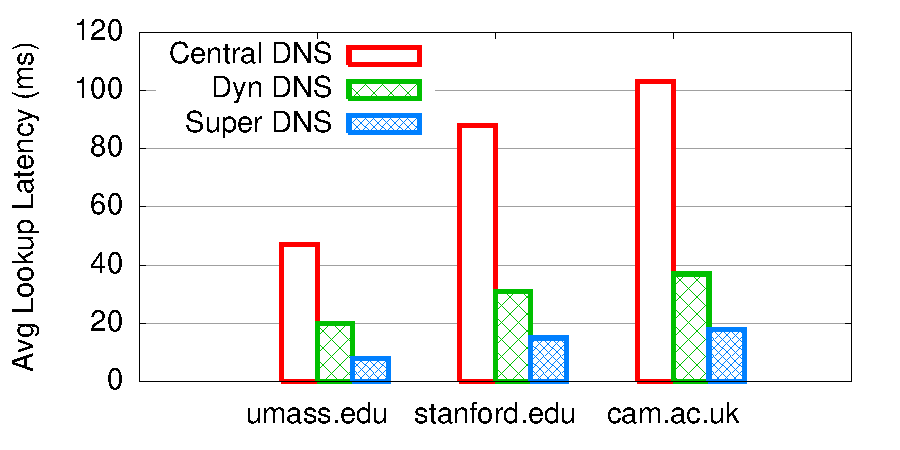
\includegraphics[scale=0.43]{graph/newgraphs/dns.pdf}
%\vspace{-0.15in}
%\caption{Managed DNS provides lower address lookup latencies than centralized authoritative name servers.}
%\label{fig:dnsmanaged}
%\vspace{-0.2in}
%\end{figure}
%
%




















\eat{
\vspace{-0.1in}
\subsection{Why not just adapt DNS?}
{\tiny{
While architectural positions like above are endlessly debatable, a more pressing question is: what if any are the limitations of DNS as a global name resolution service under high mobility and how can it be retrofitted to address those limitations?

The scalability challenge of high mobility would be felt most strongly at the authoritative name servers for two reasons. First, they would need orders of magnitude higher updates rates from mobile device names a couple orders of magnitude more in number compared to domain names today ($\approx$10B vs 146M \cite{gartner}).  Second, authoritative name servers would be unable to take advantage of TTL-based caching for  mobile device names  as much as for today's domain names.  TTLs of A-type records in DNS are more than 5 minutes for more for 40\% of records and more than 1 hour for 10\% of records\cite{Gao2013}, which implies a commensurate service outage time as updates take that much time to fully propagate. In practice, actual update rates to DNS records are orders of magnitude lower than that indicated by TTLs that are set conservatively so as to reduce outage times due to unanticipated updates; yet, ironically, outage times can often last a day or more either because of poorly planned updates or because some resolvers do not respect the TTL limits much to the woe of server administrators \cite{serverfault}. In contrast, mobile devices would require smaller TTLs to ensure reachability and can be expected to make tens of updates per day or more on average (and more frequently in short bursts such as in vehicular WiFi environments \cite{Wiffler}). Smaller TTLs imply higher load. %Due to short TTLs of mobile device names, a high fraction of lookups would reach authoritative name servers and increase their load. 

%Current DNS relies heavily on TTL-based caching to reduce address lookups to authoritative name servers. 



%Is it possible to retrofit current DNS design to provide name resolution for mobile hosts? What, if any, are the performance or scalability constraints that DNS would encounter?
\eat{
The first challenge is scalability. DNS currently manages name records for 146 million domain names \cite{whois}. To support all cell phones and tablets in the world today \cite{gartner}, DNS would have to maintain about two orders of magnitude more name records. Given the effectiveness of DNS's hierarchical and federated design in scaling by several orders of magnitude in the last three decades, one might reasonably assume that supporting more names is simply a matter of provisioning commensurately more resources at different levels of the hierarchy.

However, high mobility really throws a spanner in the works as the key to DNS scalability is its heavy reliance on TTL-based caching throughout the hierarchy. Our measurements as well as those by others suggest that DNS TTLs are more than 5 minutes or more for 40\% of records and more than 1 hour for 10\%  of records \cite{Gao2013}, which implies a commensurate service outage time as updates to resource records take that much time to fully propagate. In practice, actual update rates to DNS records are an order of magnitude lower than that indicated by TTLs that are set conservatively so as to reduce outage times due to unanticipated updates; yet, ironically, outage times can often last a day or more either because of poorly planned updates or because some resolvers do not respect the TTL limits much to the woe of server administrators \cite{serverfault}. In contrast, mobile devices would require small TTLs to ensure reachability and can be expected to make tens of updates per day or more on average, and more frequently in short bursts such as in vehicular WiFi environments \cite{Wiffler}. 

The second challenge is balancing performance and cost at authoritative name servers, the DNS tier that must bear the brunt of significantly higher update rates. 
}
%The effect of short TTLs would be felt most at the authoritative name servers, who would be frequently contacted to get the latest addresses of the mobile device.

%making DNS poorly suited for high mobility.

%To provide name resolution for mobile hosts, DNS would face two main challenges. First is the scale of the workload. DNS currently manages name records for 146 million domain names \cite{whois}. As the number of mobile devices already exceeds 1 billion \cite{gartner}, DNS would be expected to support name resolution for at least an order of magnitude more names that it does today. Given the success of DNS in scaling to a workload of size $10^8$, we expect that another  order of magnitude increase in workload could possibly be handled by provisioning more resources at every level of its hierarchy. 

To handle high mobility, we expect most end-users to outsource their authoritative name service to managed DNS providers. Managed DNS providers today are commonly geo-replicated and allow their customers to leverage better performance, availability, economies of scale, and ease of management compared to maintaining a centralized authoritative name server by themselves. However, managed DNS providers today use simplistic strategies such as {\em replicate-all} or {\em static-k} that respectively replicate a name record at all available locations or a fixed set of packaged locations (e.g. Dyn DNS offers replicate-at-all package for \$180/yr and replicate-at-4  for \$30/yr). We argue that these simplistic strategies provide poor cost-vs-performance tradeoffs even for today's (mostly) non-mobile names, a problem that will be further exacerbated by high mobility.

%Managed DNS services could offer a way to handle load on authoritative name servers.  A geo-replicated managed DNS service would have much better availability and performance than  a centralized authoritative name server.  Managed DNS providers would be able to leverage economies of scale and ease of management and would provide a more cost effective solution for mobile device names.  Desite these advantages, managed DNS providers must still manage much higher update costs of geo-replicating mobile name records. However, managed DNS providers today use simplistic strategies such as {\em replicate-all} or {\em static-k} that respectively replicate a name record at all available locations or a fixed set of packaged locations. For example, Dyn DNS offers a replicate-at-all-locations package for \$180/yr and a replicate-at-4-locations package for \$30/year. These simplistic replication strategies do not provide the best cost-vs-performance tradeoffs as shown  by the following analysis for today's domain names.

%A key cost concern for these providers in seviing mobile names would be orders of higher updates  of maintaining geo-replicated name records. 



%; these update costs are much smaller for today's domain names.
% we take . 
%The cost-vs-performance tradeoffs for managed DNS providers are apparent even today, but mobile devices names would drive up the costs of updating geo-distributed replicas by orders of magnitude, and would require strategies that provide better cost-vs-performance tradeoffs than those offered by simplistic replication strategies. 

%A centralized authoritative name server would have both poorer availability and performance, thereby necessitating a geo-replicated deployment. There would be increasing pressure on mobile device names and even small businesses and organizations to move to managed DNS providers in order to leverage economies of scale and ease of management. Managed DNS providers today employ geo-replicated authoritative name servers in order to reduce lookup latencies for their clients, e.g., twitter.com uses DynDNS \cite{dyndns}.

%could achieve better cost-vs-performance tradeoffs to handle high updates rates of  mobile device names

%To appreciate the benefit of migrating to a managed DNS provider from a centralized authoritative name server and  the limitations of managed DNS providers simplistic strategies, we take examples from today's domain names.  

To exemplify our argument for non-mobile names, consider Figure \ref{fig:dnsmanaged} that shows lookup latencies to centralized authoritative name servers of three domain names (CentralDNS), and their projected lookup latencies for two managed DNS services: (1) Dyn DNS, a leading provider with 17 known locations \cite{dnscompare}  and (2)  SuperDNS, a hypothetical managed DNS with 200 (PlanetLab) locations but replicates a name at only 17 out of the 200 locations where the domain name is highly popular. We calculate latencies based on measurements from 100 other PlanetLab locations. We measure lookup latency for Dyn at a location by querying Dyn servers for the address of twitter.com, one of its customers. The latency of SuperDNS at a location is the measured round-trip delay to the nearest replica of the name record.   We take the weighted average of lookup latencies across all locations weighted by the popularity of a domain in the geographic area (calculated using the Alexa dataset  \cite{alexa}) for which that location is geographically closest.

Unsurprisingly, managed DNS services do improve performance over a centralized service, e.g., Dyn reduces lookup latency for cam.ac.uk by 2.7$\times$. However, its simplistic replication policy leaves significant room for improvement compared to SuperDNS that leverages its massively geo-distributed deployment and intelligent replica placement, to give up to 2.5 $\times$ better performance than Dyn for the same number of replicas.
If SuperDNS were to replicate each name at all 200 locations, its update costs would increase by nearly 12$\times$.  To limit update costs, if SuperDNS were to follow a static-k policy and choose 17  locations randomly,  it would be unable to effectively use its massively geo-distributed deployment to minimize latencies.  Highly mobile device names would further exacerbate the cost-benefit tradeoffs of such simplistic replicated strategies as they would not account for the orders of magnitude higher update costs.
}}

}
%high demand for the  to be in regions of high demand for the domain name.
% that are selected in regions  selected  as per the geo-distribution of demand of the name.

%To appreciate both the benefit of migrating to a geo-replicated managed DNS provider from a centralized authoritative name server as well as the limitations of commercial managed DNS providers today, consider Figure \ref{fig:dnsmanaged}. The figure shows lookup latencies to authoritative name servers of three domain names that use a centralized server (Central DNS), and their projected lookup latencies for two managed DNS services: (1) Dyn DNS, a leading provider with 17 known locations \cite{dnscompare}  and (2)  Super DNS, a hypothetical managed DNS with 200 locations (selected from PlanetLab nodes); Super DNS replicates a name at only 17  locations that are the closest name servers selected  as per the geo-distribution of demand of the name.

%the current single location authoritative name server maintained for that name  and two alternative services: 
% assuming that its other customers would see similar performance.  

%The actual and projected lookup latencies 

% The lookup latency for a service  is the weighted average of  its lookup latencies across all locations; the weight of a location is proportional to the popularity of a domain in the geographic area for which that location is geographically closest.  

%We measure the performance of Dyn DNS at a location based on 

%The  projected performance of the managed DNS services is measured as follows: (a) Dyn DNS:  We measure lookup latency by querying Dyn servers for a domain name of one of its customers  (twitter.com) assuming that its other customers would see similar performance. (b) Super DNS:  We measure round trip latency to the nearest server at which the name record is replicated. 


%service at a location is measured as follows: (a) Central DNS: We measure lookup latencies to the authoritative name servers for the domain name. (b) Dyn DNS:  We measure lookup latency by querying Dyn servers for a domain name of one of its customers  (twitter.com) assuming that its other customers would see similar performance. (c) Super DNS:  We measure round trip latency to the nearest server at which the name record is replicated. The lookup latency for a service  is the weighted average of  its lookup latencies across all locations, where the weight of a location is proportional to the aggregate demand in the region for which that location is the geographically closest.  The geo-distribution of the demand for domain names is obtained from the  Alexa dataset  \cite{alexa}.


%To illustrate another hand-picked example, a small business in Amherst, MA \verb+www.loosegoosecafe.com+ has all four authoritative name servers in Atlanta TBD about 80ms away


%These results exemplify that it is possible to achieve better cost-performance tradeoffs than currently used simplistic replication strategies.
%Although these results are for todays domain names, they exemplify that it is possible to achieve better cost-performance tradeoffs than those offered by simplistic replication policies of today's managed DNS providers. 

%follows a replicate-all policy, it would use all 200 locations for every domain name, which would increase its update costs for keeping consistent replicas by nearly $12\times$. Alternatively, it could follow a static-k policy and choose 17  locations randomly to limit the update cost but in that case, would be unable to take advantage of its massively geo-distributed deployment to minimize latencies. 

 %DNS could be equipped to handle high mobility workloads by migrating to managed DNS services for authoritative name resolution. However, the simplistic replication strategies of today's managed DNS services leave much room for both improving performance and reducing update costs associated with  highly mobile names. 



%A managed DNS service can significantly reduce lookup latency for these domain names compared to their current single-location authoritative name servers, e.g., Dyn DNS reduces lookup latency for cam.ac.uk by 2.5$\times$.  




%
%%Performance that a domain name would see from 100 Planetlab locations if it were to use that service. 
%
%
%The geo-distribution of the demand for that domain name from Alexa dataset \cite{alexa}. For all three services, the latency shown is the weighted average of  lookup latency across all locations, where the weight of a location is proportional to the aggregate demand in the region for which that location is the geographically closest. 
%
%
%\emph{Single-location:} We calculate this latency by measuring DNS lookup latencies to the authoritative name server from 100 PlanetLab locations.  
%
%%To ensure that the average lookup latency reflects the actual geo-distribution of the DNS lookups for that domain name, we obtain city-level demand for that domain name from Alexa dataset \cite{alexa}. 
%
%
%\emph{DynDNS:} We measure the performance of Dyn from the same locations by querying Dyn servers for a domain name (twitter.com) serviced by Dyn. The performance that this domain would see for if it were to use Dyn servers is obtained by taking the weighted average of lookup latency 
%
%\emph{Managed DNS Super:} We select 17 locations that are close to the locations selected by Dyn DNS and are also close to 
%
%
%
%We measure the lookup latencies for twiiter.com domain name serviced by Dyn from PlanetLab location 
%We calculate this latency by measuring DNS lookup latencies to the authoritative name server for that domain from 100 PlanetLab locations. and by taking a weighted average of these lookup latencies based on the geo-distribution of the demand for the 
%
%
%Dyn-DNS






%The second challenge is that authoritative name servers would see many orders of magnitude larger update rates of records for mobile hosts than those seen for current domain names.  This challenge too is addressable if a small number (2-3) of replicas of authoritative name servers are maintained.  The additional update load could be supported by  provisioning more resources at authoritative name servers if necessary. To keep a small number of consistent replicas of an authoritative name server would further inflate the cost by a small factor, and hence could be supported.
%2-3, which is a manageable factor of increase in cost. Thus, for a small number of authoritative name servers, DNS appears to handle this challenge as well. 

% The  key problem with maintaining authoritative name servers at a small number of locations is that address lookups to authoritative name servers take as long as global propagation delays, i.e., hundreds of milliseconds, and result in increased connection setup times. The state-of-the-art solutions for authoritative name servers, managed DNS providers \cite{ultradns, dyndns, dnsmadeeasy}, address this problem by deploying servers at a few tens of locations globally and replicating name records from their customers at all locations.  These providers provide authoritative DNS service for  many of the top enterprises today.
 
% If these providers were to provide authoritative name service for mobile hosts, their current design makes it extremely hard for them to provide  a cost-effective, and high performance  service due to following reasons:
 
%The current design of managed DNS providers makes it extremely hard for them to provide  a cost-effective, and high performance  service for all mobile hosts in the Internet. These providers would incur excessively high update cost at each location due to their policy of replicating name records at all locations. For example, processing 100M updates/sec from 10 billion mobile devices alone would require thousands of machines to be deployed at every location. This "replicate-everywhere" policy entails that the deployment consists of a small number of locations each of the size of a large data center. Thus, due to high update costs associated with adding new locations, it would be much more costly to maintain even their current deployment of tens of locations across the globe;   and  infeasible to have a massively geo-distributed deployment at hundreds or thousands of locations, e.g. Akamai's servers are deployed at more than 10000 locations, that provides small lookup latencies (few ms) to users across the globe. 

%While high mobility of end-hosts makes it costlier to have more deployments, managed DNS providers do have considerable room for reducing lookup latencies with a more geo-distributed deployment of servers. We measured the address lookup latency to authoritative name servers for 318 domain names that are serviced by a leading managed DNS provider. These measurements were done from 100 PlanetLab locations by sending a total of 1000 lookups for each domain name across all locations. Figure \ref{fig:lookuplocation} shows the distribution of median lookup latencies at all locations. Lookup latency is more than 100 ms from  30\% percent of the locations. This finding suggests that the current deployment of managed DNS providers, due to a limited geo-distribution of their servers, does not fully address the problem of high lookup latencies to the authoritative name servers.



%\begin{figure}
%\centering
%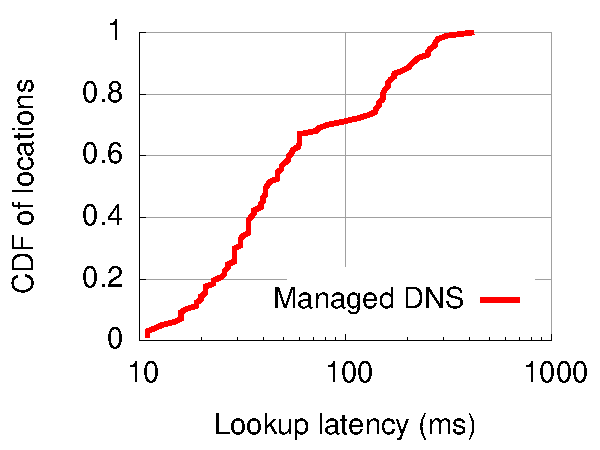
\includegraphics[scale=0.5]{graph/newgraphs/lookup-location.pdf}
%\vspace{-0.1in}
%\caption{Distribution of latency of lookups to authoritative name servers of a managed DNS provider from 100 Planetlab locations.}
%\label{fig:lookuplocation}
%\vspace{-0.1in}
%\end{figure}


% from 100 PlanetLab locations to authoritative name servers  for 318 domain names that are serviced by a leading managed DNS provider (refer to Section \ref{sec:managed}). 
%This finding suggests that managed DNS providers have considerable room for reducing lookup latencies with a more geo-distributed deployment of servers.

%In summary, the current DNS design could be used to provide name resolution for mobile hosts but would continue to face the problem of high lookup latency to the authoritative name servers. Having a massively geo-distributed deployment of authoritative name servers could provide low lookup latencies across the globe, but prohibitively high update costs associated with mobility makes it infeasible for managed DNS providers to support such a deployment in a cost-effective manner.


%
%
%
%For the name records of mobile hosts, authoritative name servers would see an update rate that is orders of magnitude higher than those of currently existing records in DNS.  over-provision authoritative name servers to solve the problem. 
%Second problem, which plagues name DNS even today is that lookups to authoritative name servers results in high latencies. 
%
%



%%%%%%%%%%%%%previous version of this section%%%%%%%%%%%%%

\eat{
Providing name resolution for mobile hosts would present DNS with a workload with very different characteristics than that of today's DNS.
For the name records of mobile hosts, authoritative name servers would see an update rate that is orders of magnitude higher than those of currently existing records in DNS. 
Frequent address updates by mobile hosts imply that cached addresses could be reused for much shorter durations. A record for a user that changes networks 100 times a day could be reused only for 15 minutes on average, after which a fresh name record must be fetched from the authoritative name servers. Frequent lookups to authoritative name servers, besides increasing the load on authoritative name servers, would increase connection setup time to mobile hosts. For example, if the authoritative name server is maintained at a single location, address lookups may take of the order of global propagation delays, e.g., 100s of milliseconds. Increased load of lookups and updates on authoritative name servers could be managed by provisioning more resources at authoritative name servers, but high lookup latency to authoritative name servers remains the primary problem for current DNS.
%Therefore,  is a challenge, even though provisioning  more resources at authoritative name servers could help cater to an increased load.


The state-of-the-art solutions for authoritative name servers are provided by managed DNS providers. These providers maintain servers at a few tens of locations globally and replicate name records from their customers at all locations.  These providers handle the DNS service on behalf of many of the top enterprises today. 
However, the currently available the managed DNS provider solutions have two main shortcomings: 

(1) Due to a limited geo-distribution of their servers, managed DNS providers do not fully address the problem of high lookup latencies to the authoritative name servers. We measured lookup latency to authoritative name servers for 318 domain names that are serviced by a leading managed DNS provider from 150 PlanetLab locations. Figure 1 shows the distribution of lookup latencies in our measurements. 30\% percent of lookups take more than 100 ms. 
%authoritative name servers managed DNS providers from 150 PlanetLab locations to 318 domain names in the top 10K websites as per Alexa ranking; these names are served by a leading managed DNS provider.

%For instance, to connected to a mobile host who is 10 ms away, may need a lookup that is 150 ms or even more.


(2) These providers would incur excessively high update cost at each location due to their policy of replicating name records at all locations. For example, processing 100M updates/sec from 10 billion mobile devices alone would require thousands of machines to be deployed at every location. This "replicate-everywhere" policy entails that the deployment consists of a small number of locations each of the size of a large data center. Thus, due to high update costs associated with adding new locations, it is infeasible to have a massively geo-distributed deployment at thousands of locations, e.g. Akamai has 10000 locations, that provides small lookup latencies to users across the globe. 

In summary, the current DNS design is ill-suited to provide name resolution for mobile hosts due to high lookup latencies to authoritative name servers. Having a massively geo-distributed deployment of authoritative name servers could provide low lookup latencies across the globe, but prohibitively high update costs preclude such a deployment. 
}

%%!TEX root = New.tex
\section{Naming in MobilityFirst}
\label{sec:MF}

In this section, we describe the design of the naming subsystem in MobilityFirst, which forms an important part of the motivation for \auspice. %Readers uninterested in future-Internet-architectural usage scenarios can skip to Section \ref{sec:auspice} with minimal loss of continuity.

A {\em name} in MobilityFirst is a {\em globally unique identifier} (GUID) that can be used to identify a variety of {\em principals} such as an interface, a device (or the set of all interfaces on the device), a service (e.g., HTTP), an end-user (or the set of all devices owned by the user), a network location, or named content. 

\textbf{Certification, addressing, and routing.} A GUID is self-certifying, i.e., any principal can authenticate another principal claiming a GUID without the need for third-party certification. A self-certifying GUID is derived simply as a one-way hash of a public key, so a GUID can be authenticated using just a bilateral challenge/response step as only the authentic principal possesses the corresponding private key. 

Self-certifying identifiers do not obviate certification authorities. In addition to a GUID, a principal may be assigned an optional human-readable name (e.g., ``www.amazon.com'' or ``Tom Sawyer's cell phone'')  or an inexact intent (e.g., a set of search keywords or other abstract descriptions). In such cases, {\em name certification services} bind the human-readable name or intent to a public key, and end-users or applications must first obtain such a certificate from a service they trust.

A {\em network address} (NA) is a self-certifying identifier for a network or an autonomous domain. The tuple [GUID, NA] is a routable destination address carried in packet headers. Senders query the name service to obtain the NA corresponding to a GUID (much like they query DNS to obtain the current IP address corresponding to a domain name) before sending the first packet to the destination. Senders are also permitted to send a packet addressed just to a GUID, thereby implicitly delegating to the first-hop router the task of querying the name service for the corresponding NA. End-to-end packet forwarding is accomplished by an interdomain routing protocol that delivers packets to the destination NA (oblivious of the destination GUID) and subsequently by an intradomain routing protocol that delivers the packet to the destination GUID.

\textbf{Hierarchical routing.} The interdomain routing protocol enables reachability to NAs much like the current Internet enables reachability to IP prefixes. Thus, the number of forwarding table entries in a core router is the total number of NAs. As the number of NAs may grow significantly over time (e.g., home networks, vehicular networks, body area networks, etc.), the interdomain routing protocol is designed to support a small number of levels of hierarchy so as to trade off packet header space against forwarding table size. An interdomain routing hierarchy with two levels as in our current implementation consists of  {\em core} and {\em edge} networks. The name service translates a GUID into a two-tuple $[X, T]$ where $X$ is the last core network enroute to $T$, the terminal network to which the GUID is attached. Core networks only maintain forwarding entries for other core networks and a small number of their ``customer'' edge networks while edge networks need maintain forwarding entries only for a small number of their ``provider'' core networks and edge networks in their vicinity.

\textbf{Multihoming.} A multi-homed GUID is simultaneously attached to more than one core or terminal network. In these cases, the name service by default returns a list of all homes of the form: $\{[X_1, T_1], [X_2, T_2], \ldots \}$. Multi-homed GUIDs can also specify expressive policies for engineering incoming traffic, e.g., prefer WiFi to 3G; or WiFi for delay-tolerant downloads and 3G for delay-sensitive traffic, etc. Network operators can explicitly create NAs for portions of their network and specify incoming traffic engineering policies instead of abusing longest-prefix matching as commonly practiced today.

\textbf{Content retrieval.} Content in MobilityFirst is also named using a self-certifying identifier, but a content GUID is simply the hash of the content itself. This widely used technique \cite{BitTorrent} obviates the need for public keys for verifying the authenticity of static content. Given a content GUID, the name service returns a list of network addresses $\{[X_1, T_1], [X_2, T_2], \ldots \}$ from where replicas of a content may be fetched. The list of these locations typically only includes replicas maintained by content providers or their delegates, however any network intermediary can intercept a content request and serve the content if it possesses a cached copy.

\textbf{Indirection and grouping.} Indirection enables the name service to resolve a GUID to another GUID and grouping allow a set of GUIDs to be a assigned a single GUID. Indirection and grouping are powerful operations that enable GUIDs to support new network primitives in an efficient manner. We illustrate these benefits using three examples: 

(1) {\em Multicast}: A multicast GUID (MGUID) has the same format as a regular GUID and the resolved output of the name service has the same format as multi-homed network address. However, the resolution procedure and routing are different as follows. The name service maintains a membership set for each MGUID that consists of all GUIDs subscribed to the multicast group. Each member GUID $i$ in MGUID subscribes to the group via a single home, $NA_i$. The name service resolves an MGUID by returning the union of all $NA_i$'s that have at least one GUID subscribed to the MGUID. By default, the sender is responsible for sending data addressed to $[\textit{MGUID}, NA_i]$ for each of the returned $\textit{NA}_i$'s. When packets arrive at a destination $\textit{NA}_i$, the $\textit{NA}_i$ is responsible for resolving the MGUID to the subset of member GUIDs attached to its network and forwarding a copy to each member. Geo-casting, e.g., sending a message to all yellow cabs near Times Square, and other context-aware services can be supported in a similar manner by having the name service maintain geolocation or context attributes in addition to network locations of GUIDs.

(2) {\em Content directories}: Content is typically organized in hierarchical name spaces, e.g., www.nytimes.com/sports, www.nytimes.com/business, and so on, to enable grouping and colocation of related content. However, as GUIDs do not capture locality, moving the location of a large content directory from one network domain to another will by default result in updates to all of the constituent content GUIDs. To reduce this overhead, a set of content GUIDs can be assigned a directory GUID, in which case the name service maintains network addresses only for the directory GUID and returns it upon a request for any constituent content GUID.

(3) {\em Grouping}: Affinity groups as for content above help reduce the overhead of maintaining network locations for any group of GUIDs, e.g., a group of interfaces in an airplane, even when no data transfers are actually taking place. Thus, any group of colocated GUIDs can be assigned a group GUID that requires only one update for the entire group every time the network location of the group changes.

\textbf{Access control:} The name service controls access to network addresses as well as other attributes (such as geolocation, traffic engineering preferences, etc.) of a GUID by allowing the owner (or any entity possessing the corresponding private key) to specify access control policies for the GUID's stored attributes. The owner can specify either a blacklist or whitelist for read or write access to each stored attribute.

%%!TEX root = New.tex
\section{The \auspice\ service placement engine}

A key distributed systems challenge in realizing a global name service as described above is the design and implementation of a scalable resolution infrastructure to rapidly resolve identifiers to attributes. To address this challenge, we develop \auspice, a system that automates geo-distributed placement of resolver replicas in a locality and load-aware manner.

\subsection{Design goals and challenges}
\label{sec:design_goals}

An automated resolver replica placement system must satisfy the following design goals.

\begin{enumerate}

\item {\em Low response time}: Replicas of each resolver should be placed close to its end-users so as to minimize user-perceived response times.%\vsp
\item {\em Low update cost}: The number of replicas of each resolver should be controlled so as to limit the update cost required to maintain replica consistency. 
%\vsp
\item {\em Load balance}: The placement of resolver replicas and redirection of client requests should ensure that no single name server location becomes a hotspot.%\vsp
\item {\em Fault-tolerance}: A sufficient number of active or dormant replicas of each resolver must be maintained so as to satisfy its availability objective.
%\vsp
\item {\em Consistency}: The system must achieve the above objectives while respecting the consistency requirements of each resolver.

\end{enumerate}

Although each of the above goals is straightforward and shared by a number of other distributed systems, satisfying the combination of goals is rather challenging. To appreciate why, consider a few straw man alternatives: 

(1) {\em Replicate everything everywhere}: This scheme can minimize response times but can induce a prohibitively high update cost as well as load imbalance. 

(2) {\em Authoritative resolvers(s) plus edge caching}: This scheme maintains one (or a small number of) authoritative resolvers for every name record (similar to today's DNS) and a large number local name servers pull data infrequently from authoritative resolvers. This approach can reduce update bandwidth cost by reusing stale, cached copies of the service's data, however consistency requirements may prevent or severely limit these cost savings, e.g., a mobile host''s name record that is updated frequently may soon become stale requiring a local name server to frequently contact the authoritative resolvers.

%Even for services with weak consistency requirements (e.g., online catalogs), the placement system needs to balance the trade-off between response times and load balance for compute-intensive services.

(2) {\em Consistent hashing with replication}: This approach (e.g., \cite{consistent-hashing}) can ensure load balance and fault-tolerance but may incur high response times as the load balance benefits of randomization are fundamentally at odds with placing resolvers in a locality-aware manner \cite{codons,cox, beehive}. Significantly increasing the number of resolvers  can improve response times but also increase update cost for write-intensive services.

In accordance with our design goals, Auspice explicitly determines the number and placement of resolver replicas for an identifier taking into account its query and update rates and the geographic locality of queries, and redirects client requests taking into account the aggregate load at each name server. We describe this design in detail in section TBD.


\begin{figure}[t]
\centering
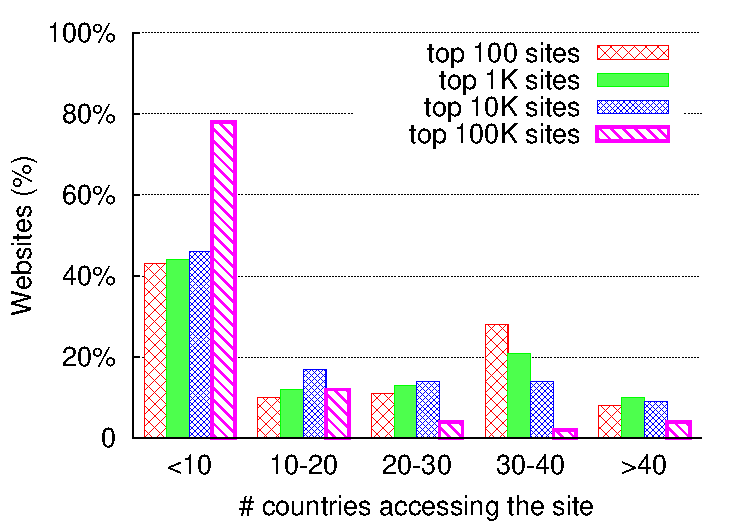
\includegraphics[scale=0.6]{figure/numcountry_boxplot.pdf}
\vspace{-0.1in}
\caption{Locality in website popularity: 40\% websites are accessed in less than 10 countries.}
\label{fig:localityweb}
\end{figure}


\subsection{Geographic locality}

%Replicating name records in locality-aware manner minimizes request latencies as well as update costs. 
If request patterns show geo-locality, placing a small number of resolvers in a locality-aware manner achieves low request latencies; the cost of keeping resolvers updated is minimized by creating a small number of resolvers. Our analysis of of geo-distribution of today's websites' traffic suggests that request patterns for their name records  show a high degree of geo-locality\tbd{Do you have a breakdown by grids of fixed size? Countries can vary greatly in size. Also, are google and facebook accessed in just 40 countries? This seems very likely wrong.}. We argue that name records for mobile hosts are likely to show even stronger geo-locality patterns, thereby making the case for a locality-aware placement of resolvers\tbd{On what basis are you arguing? Do you have a reference or a justification?}.

%Our design is motivated in part by two key features of the workload that the naming service is expected to handle: high update rates of name records, and geo-locality of distribution of requests.  A mobile host rapidly changes the set of networks it is connected to and thus requires frequent updates to its name record. 
 
\begin{table}[t]
\centering
\begin{tabular}{ l | c | c}
\hline
rank \& site & \# countries & country most accessed\\
  & accessing  & \& traffic percentage\\
\hline
\hline
1, google.com & 36 & US \ 37.3\% \\ 
\hline
2, facebook.com & 40 & US \ 19.6\% \\
\hline
3, youtube.com & 39 & US \ 19.1\% \\
\hline
4, yahoo.com & 31 & US \ 32.8\% \\
\hline
\rowcolor[gray]{0.9} 5, baidu.com & 5 & CN \ 96.8\% \\
\hline
6, wikipedia.org & 34 & US \ 19.9\% \\
\hline
7, live.com & 33 & US \ 15.3\%\\
\hline
\rowcolor[gray]{0.9} 8, amazon.com & 19 & US \ 74.9\%\\
\hline
\rowcolor[gray]{0.9} 9, qq.com & 5 & CN \ 95.5\%\\
\hline
10, twitter.com & 31 & US \ 26.4\%\\
 \hline
\end{tabular}
\caption{Locality in top 10 sites: two sites baidu.com and qq.com have 95\% traffic coming from a single country.}
\label{tab:top10web}
\end{table}

 
We analyze geo-locality of today's websites using Alexa TopSites dataset  \cite{alexa}, which provides ranking of today's top websites, and geo-distribution  of  each website's requests. These statistics are based on page views for each website, but we expect the number of name record requests for a website to be proportional  (or positively correlated) to its page views in a geographic region. 


Figure \ref{fig:localityweb} shows the geo-locality in website popularity: it plots the percentage of websites that are accessed in different numbers of countries. 40\% websites are accessed in less than 10 countries for the top 100, 1K, 10K sites and the percentage value goes up to 80\% for the top 100K sites.  Table \ref{tab:top10web} further zooms into the access statistics for the top 10 popular websites. Geo-locality persists in the top 10 sites and is prominent for three sites: baidu.com and qq.com which have 95\% traffic coming from a single country China and amazon.com which has 75\% traffic coming from United States.
Thus, a locality-aware placement of resolvers is a natural choice, e.g., China for baidu.com and qq.com and US for amazon.com.

The name record of a mobile host (\emph{mobile name} for short) is likely to show a strong geo-locality of requests. This is due to several reasons.
Updates for mobile names will originate from the mobile host itself, whose mobility will be contained in a small geographic region for most hosts.
Lookups for a mobile name will be done by web services to push updates to the mobile host. Today's web services are geo-replicated to position themselves closer to end-users. Most likely, the closest service replica will lookup for the mobile name, giving rise to geo-locality.
Another source of a mobile name's queries is communication between two mobile hosts, e.g., a user's friends contacting the user's mobile device to send messages.
We expect these queries to come from a user's contacts list. Since most of a user's contacts are expected to be within  the same country, these  queries will exhibit strong geo-locality patterns as well.


\eat{
\subsection{Geo-distributed cloud services}
Geo-distributed computing clouds today offer a scalable and cost-effective solution for hosting a variety of online services such as search, social networking, web portals, e-commerce, etc. These clouds are typically hosted by a large hosting service provider that is responsible for allocating resources on demand to a large number of hosted enterprise services. Examples of such hosting environments include Amazon's AWS suite \cite{amazonec2}, Google's AppEngine \cite{google-app-engine}, Akamai's Edge Computing \cite{edgecomputing}, and Windows Azure \cite{windowsazure}. The hosted services benefit from economies of scale, agile provisioning of on-demand resources, and ease of management that comes with cloud hosting. Geo-distributed clouds are particularly attractive as they enable hosted services to locate themselves close to their end-users, thereby significantly improving user-perceived latency.

To appreciate it, we performed a large scale case study on two cloud-based services --- naming service for Alexa TopSites and online social networking service for Twitter users. Alexa TopSites \cite{alexa} provides lists of web sites ranked by their worldwide traffic statistics. Each website relies on a naming service to direct requests to appropriate name resolvers.
Users of Twitter \cite{twitter} depends on the underlying social networking service infrastructure to deliver status updates that they share ideas, activities and events with their friends. 
A more detailed description of how we collect data from these services is deferred to section \ref{sec:eval}. Our explored study based on 100,000 Alexa websites and TBD Twitter users reveal strong localities in user access pattern, a feature that can benefit significantly by agile service placement.

Figure \ref{fig:localityweb} shows the locality in website popularity: it plots the percentage of websites that are accessed in different numbers of countries. 40\% websites are accessed in less than 10 countries for the top 100, 1K, 10K sites and the percentage value goes up to 80\% for the top 100K sites. 
Table \ref{tab:top10web} further zooms into the access statistics for the top 10 popular websites. The first and second columns show the rank, name and number of countries that access a site, and the third column shows the country that accesses the site most and its corresponding traffic percentage. Locality persist in the top 10 sites and is prominent for three sites: baidu.com and qq.com which have 95\% traffic coming from a single country China and amazon.com which has 75\% traffic coming from United States.
Thus, it is natural for a website naming service to place resolver replicas close to pockets of demand, e.g., China for baidu.com and qq.com and US for amazon.com.

However, a critical limitation of geo-distributed clouds today is that each hosted service has to manually determine the geographic locations of replicas of their service. Hosted services typically select these locations by monitoring the geolocations of end-user requests at coarse-grained timescales (e.g., several weeks or months) and creating new replicas or migrating existing ones close to regions of heavy demand. Furthermore, as each hosted service determines its replica locations independently, the hosting service provider may experience hotspots at one or more locations resulting in SLA violations and revenue loss.

Our position is that service replica placement for hosted services can and should be automated by hosting service providers. Automated placement obviates redundant effort on part of hosted services and enables the hosting service provider to manage its global resources in a more efficient and agile manner.
}


% related to service placement.
\eat{
Clearly, it is not easy to design a general-purpose placement engine that can satisfy all of the above goals for arbitrary services. So, we restrict the scope of this paper to services with a single bottleneck resource. This restriction allows us to measure the demand for each service and the available capacity at each hosting site with a scalar metric, e.g., the demand for each service and the aggregate capacity at a site can be measured in requests/sec. Note that this restriction does not imply that the services or requests have to be homogeneous, only that their aggregate demand can be specified as a scalar. For example, suppose service A  is a web server with a demand of 250 requests/sec and the maximum sustainable throughput for service A (in isolation) at the site is 1000 requests/sec, and service B is a database server with a demand of 80 queries/sec with a corresponding maximum sustainable throughput of 400 queries/sec. Further suppose that both services are bottlenecked by a single resource, e.g. they are both compute-bottlenecked or they are both IO-bottlenecked or they are both bandwidth-bottlenecked. In this example, it is straightforward to see that the site has enough capacity to place both services as service A uses 25\% of the capacity and service B uses 20\% of the capacity.

Although the above assumption allows us to accommodate a large class of services and hosting scenarios, it does limit the types of supportable services. For example, suppose service A is memory-bottlenecked and has a demand corresponding to 75\% of the maximum throughput sustainable for A alone at that location, and service B is network-bandwidth-bottlenecked with a demand corresponding to 80\% of the maximum sustainable throughput for B alone. Without additional information about each service, it is not possible to determine if both A and B can be placed at the location. More importantly, even if one could measure the usage of each resource for each service, the distributed nature of the problem makes load balancing in scenarios with such ``multi-dimensional'' resource constraints much harder. As a result, the problem of automatically placing arbitrary services (and in particular virtual machines running ``black-box'' services) is not within the scope of \auspice's design.
}

\eat{
% why DNS will not work.
A global  name resolution service for mobile hosts requires a radically different design than the current DNS, which caters to immobile hosts whose network addresses are updated infrequently. 
The current DNS design manages to provide an acceptable performance due to heavy reliance on TTL-based caching.
Name records for mobile hosts would be updated at orders of magnitude higher rates than name records in today's  DNS. For example, a mobile host may change network addresses tens of times per day, while a domain name's IP address does not change for weeks or even months.
A high update rate of name records dictates that TTL values are set to orders of magnitude shorter values, e.g. few seconds instead of 6 hours or one day. In the current DNS design, short TTLs will cause requests for name records of mobile hosts to frequently contact a small number of authoritative name servers for that name record, resulting in very high latencies.

% replicate-all high costs
An obvious solution to improve performance is to replicate every name record at a large number of locations around the globe. However, maintaining the consistency of a large number of name record resolvers increases the update cost,  both in terms of network bandwidth and server resources.
The update cost would be manageable if the name record is updated infrequently such as  the current DNS's  name records.
The update costs for billions of mobile devices, updating addresses up to 100 times per day,  would require processing a million updates per second at every location.
Clearly, a ``replicate everywhere'' strategy would, at best, add substantial costs to the service, or might even be infeasible. 

% intuition behind our design
This leads us to ask if we can design a replication strategy with much smaller cost of updates that yet achieves small response latency. As the update cost increase with the  rate at which a name record is updated, this suggests that the number of resolvers of a name record should be inversely proportional to its update rate. By this thumb rule, the name  record of a mobile host has a high update rate and therefore must be replicated at a small number of locations.

To provide low response latencies with a small number of resolvers, resolvers must be located close to the pockets of demand. This rules out designs that augment consistent hashing with a small amount of replication \cite{codons,cox, beehive}. These designs can ensure load balance and fault-tolerance but may incur high response times as the load balance benefits of randomization are fundamentally at odds with placing resolvers in a locality-aware manner. In this paper, we propose an approach that explicitly measures the geo-distribution of  requests and replicates name records in a locality and load-aware manner. This results in an order-of-magnitude lower update costs than a replicate everywhere scheme, and yet achieves close to the best response latencies.
 }

\chapter{Demand-Aware Geo-Distributed Placement for Low Latency}
\label{ch:auspice}

Geo-distributed computing clouds such as Amazon EC2, Google offer a scalable, fault tolerant and flexible solution for hosting web services that cater to users world-wide. The easy availability of these platforms provides opportunities to several applications to leverage the performance benefits of geo-distribution.

A challenge for a web service in switching to a geo-distributed cloud is the cost of replication of the ``data-tier''. Several web services today generate dynamic content such as weather information, stock prices, and status updates posted by users on a social networking website. Data replication is necessary to reduce latency of content accesses but is a costly operation for dynamic content. The reason is that the cost of propagating updates to dynamic content increases linearly with the number of locations. State-of-art replication alternatives either provide poor cost-vs-performance tradeoffs or leave data placement to be done manually by web-services which increases human cost and effort. For example, DHT-based designs make a constant number of replicas but result in high latency of content accesses.


Our key insight is that replication of dynamic data should be done in a demand-aware manner such that a limited number of data replicas placed close to pockets of demand are sufficient to reduce latency of content accesses. A demand-aware placement implicitly assumes geo-locality of workloads, an assumption we believe is justified based on recent studies of workload characteristics. We have developed a heuristic placement strategy that decides number of replicas based on read-to-write ratio of a name and selects replica locations based on geo-distribution of demand to provide low lookup latency, low update cost, and high availability.


Our system, \auspice, is implemented as a geo-distributed key-value store that stores arbitrary JSON objects as records. Like several other key-value stores \cite{mongodb,Escriva,cassandra}, \auspice\ exposes a simple GET/PUT interface to clients. \auspice\ provides flexible consistency semantics for accesses to a single object. However, \auspice\ is not a general-purpose database and lacks several features that are common in a database, e.g., support for running SELECT queries efficiently, or support for transactions. 
\auspice\ is scalable to a large number of locations and data items due to a fully decentralized design both in the data plane and and the control plane that makes data placement decisions. 

An application suited for \auspice\ is a global name service that provide name-to-address mapping for mobile devices. We have evaluated \auspice\ extensively for an expected workload of such a global name service. Our experiments show that \auspice\ provides  5.4$\times$-11.2$\times$ lower lookup latency than a DHT-based design for DNS. In a comparison to commercial managed DNS providers, we find that \auspice\ 
provides a median update latency that is 1.1 sec to 24.7 sec lower than three top-tier providers.

%!TEX root = New.tex
\section{\shrink\ Design}

\shrink\ is a cluster manager that handles traffic engineering, load balancing and power management in CDN datacenters for maximizing energy savings with minimal effect on user-perceived performance or hardware reliability. This section provides an architectural overview of the system,  the CDN datacenter model on which \shrink's design is based, the energy,  performance, and reliability metrics which \shrink\ optimizes.


\subsection{Architectural overview}

\shrink\ is a cluster manager software which runs at the front-end load balancer. \shrink\ requires support from daemon processes running at each server for reporting content demand statistics to \shrink\ and to execute content transfer decisions sent to it. \shrink\ also requires datacenter switches to support OpenFlow in order to implement its traffic engineering decisions. 
The functionality to support powering on/off switches and servers is implemented via TBD and TBD respectively. Servers at the datacenter periodically report content demand statistics to \shrink, based on which it computes a set of load balancing, traffic engineering and content transfer decisions, and also decides which set of servers and switches to keep active in the next interval. The computed load balancing decisions are updated locally, and servers and switches are informed of the updated content transfer and traffic engineering decisions respectively. When all servers report that content transfer is complete, \shrink\ informs switches and servers to turn on/off as necessary.

\subsection{CDN datacenter model}

Table 1 lists all the model parameters. 
A CDN datacenter consists of a set of nodes $V$, which are either servers $S$ or switches $R$. The nodes are connected by a set of directed edges $E$ that represent the datacenter network links. All servers are homogenous and have a storage  $D$ and can serve traffic at a peak capacity of $B$ (in bits/sec).  Each link $e\in E$ has a capacity  $C_e$.

The set of content requested by end-users is represented by the set $K$ and the sizes of content are denoted by $S_k, k\in K$.  A demand vector $T$ specifies the demand for each content, such that the $k$-th entry of this vector $T_k$ denotes the demand for content $k\in K$.

The rest of the Internet excluding this datacenter, which includes end-users and other data centers, are modeled as virtual node $o$. The virtual node connects to the root nodes in datacenter network via virtual links which are assumed to have very high capacity. Content requested by clients are sent from servers via root nodes to this virtual node $o$. Also, any content that is unavailable within the datacenter can be fetched from the virtual node $o$ to  any server in the datacenter.

\textbf{Energy model:}  Our energy models reflects typical power usage  of switches and servers. The energy use of a switch  $i \in R$ that is turned on  $PR_i$. A switch consumes the same amount of energy independent of the rate at which it is forwarding traffic. Indeed, several  switch vendors report that their switches consume in excess of 90\% of their peak power in idle state. A server $i \in S$ consumes a fraction $f$ of its peak power $PS_i$ when idle. As server utilization increases from 0\% to 100\%, server's energy use grows linearly from $f\times PS_i$ to $PS_i$. 

%is the sum of energy consumption of the chassis  and of the line cards plugged into the chassis.  All routers have a similar chassis which consumes $R$ units of energy, the line card for link $e \in E$ uses $L_e$ energy units on routers at both ends.

%Energy consumption of a server in use in $P$ watts. At any time, only a subset of servers at a PoP are turned on at any time to reduce energy use. Total energy use of servers at a PoP is $P$ times the number of servers that are turned on.


\subsection{Problem statement}

\shrink's goal is to minimize the energy use of server and network components in a datacenter. Moreover, the system must meet following performance and reliability constraints: 
\begin{itemize}
\item
We target to provide three-nines of server availability, which is a common SLA guarantee provided by CDNs. A server is said to be available to serve a request if it has enough spare resources to start serving the request without delay.
\item
Requests that require the content to be fetched from servers outside datacenters and incur a high latency for the end-user. We seek to ensure that  the fraction of such requests increases by no more than a small percentage ($\approx 10\%$) compared to the current CDN policy of keeping entire datacenters in an always on state.
\item
Transitions between on and off states cause wear-and-tear and reduce hardware reliability. We aim to keep the frequency of on/off transitions of a server or a switch to less than once per day.
\end{itemize}

% What about fault tolerance goals?

Towards achieving above goals, \shrink\ makes following set of decisions that are formally defined below:

%The set of decisions made by \shrink\ are formally defined as follows: 
\emph{Power management:} Compute binary variables $p_i, i \in V$ to decide whether servers and switches are powered on  ($p_i = 1$) or off ($p_i = 0$).

\emph{Load balancing:} Compute variables  $l_{ks} \forall k \in K, \forall  s \in S$ such that $\sum_k l_{ks} = 1$, where $l_{ks}$ denotes the fraction of requests for content $k$ that are sent to server $s$.

\emph{Traffic engineering:} Compute routing between nodes $i,j \in V \cup \{o\}$ by deciding variables  $f_{ije} \forall i,j \in V \cup \{o\} \forall e\in E$, which denote the fraction of traffic from $i$ to $j$ that flows on link $e$.

\emph{Pre-shutdown content transfer:} Compute the set of content transfers to be done prior to shutdown of a set of servers, where a content transfer is defined by a three-tuple $(k, i, j)$, which denotes that content $k \in K$ is to be copied from server $i \in S'$, to sever $j \in S''$, where $S'$ is the set of servers being shutdown at a current stage  and $S''$  is the set of servers that will remain active post-shutdown. 

\eat{
(1) Select number of servers to keep on considering both cache hit rates and aggregate load. T is a parameter, that is empirically defined. 

(2) Select number of components that are kept active using an optimization algorithm. Coordinated server and network shutdown. Retain same components as much as possible. 

(3) Load balancing algorithm. Describe how we account for server-to-server traffic. Minimum number for fault-tolerance. Making load-balancing energy-aware. 

(4) (Content transfers?)

(5) Traffic engineering is simple.


}
\subsection{Algorithms}
\label{sec:heuristic}

With some simplifications, we have formulated the optimal strategy for the above problem as a mixed-integer program. But, we find that the optimal strategy takes tens of minutes to compute a solution even for a small-scale datacenter with few tens of nodes, and could fail to meet the three-nines availability goal in case of sudden spikes in content demand. Therefore, \shrink\ uses a set of computationally efficient heuristics to make all the above decisions which are described next. A description of the optimal strategy is presented in the Appendix \ref{sec:optimal}.

\eat{
Define a complete system which meets the above stated goals:

(1) How many servers to keep on?

(2) How to do load balancing decisions?

(3) How do decide which parts of network to keep on?

(4) How to make traffic engineering decisions?

(5) Which content to transfer before server shutdown?
}

\subsubsection{Power management}


%Power management consists of two decisions: deciding number of servers to keep on, and selecting which set of servers,  and switches to keep active. 

\shrink's power management policy is composed of two algorithms. The first algorithm decides the number of servers to be kept active, based on which the second algorithm decides which set of servers and switches are to be turned on or off. 
%Both algorithms try to maximize energy savings while reducing the number of on-off transitions.


%Our strategy is similar to those proposed by others, e.g., Matthew et al., and turn on a server immediately if average load increases over a given level, and shuts off a sever that has been unused for the past hour. The former minimizes affecting server availability, and the later reduces impact on hardware reliability.  
%The number of active servers are decided using an online algorithm whose input is a time-series of aggregate load on datacenter. A data point in this time series reflects the load in a 1-minute window and is calculated by summing the utilizations reported by all servers in that window.

*** Don't begin with Matthew et al.***

The number of active servers are decided using an online algorithm proposed by Mathew \emph{et al.}  \cite{mathew12} whose input is a time series of aggregate load on datacenter. A data point in this time series reflects the load in a one-minute window and is calculated by summing the utilizations reported by all servers in that window. The algorithm run at one-minute intervals and decides to turn servers on or off based on three values: aggregate load in the previous minute $L\_PREV$, maximum aggregate load in the previous hour $L\_MAX$, and the current number of active servers $N$. $L\_PREV$ and $L\_MAX$ are measured relative to the capacity of a single server. If $L\_PREV > \alpha N$, turn on $\lceil \frac{L\_PREV - \alpha N}{\alpha} \rceil $ more servers. if  $L\_MAX < \alpha N$, turn off $\lceil \frac{\alpha N - L\_MAX}{\alpha} \rceil$ servers. When load increases, the algorithm immediately turns more servers on to minimize the impact on server availability.  When load decreases, the algorithm waits for an hour to see if the decrease in load persists before turning servers off, a strategy which reduces the number of on-off transitions due to a spurious decrease in load.
%If the decrease in load is spurious, this strategy avoids unnecessary on-off transitions.


Algorithm \ref{algo:power} presents the pseudocode for the algorithm to select the active switches and servers based on the number of active servers N. The N active servers are chosen to be the N leftmost leaf nodes. Thereafter, the algorithm selects a subtree in the topology with following three properties: (1) Only these N nodes are the leaf nodes. (2) The sum of link capacities between nodes at successive levels is at least as much as the sum of outgoing link capacities of active servers. This property ensures that enough switches are active at each level so that  even if all servers send data at their outgoing link capacity, there are no bottleneck links. (3) 
*** don't start with Is***

****  if we use colon " : ". bullets should be compact sentences. ****

****  

*** good subtrees = (1) and (2)  *******
Is the subtree with the minimum number of nodes, which satisfies properties (1) and (2). The third property minimizes network energy use. 
This algorithm implicitly depends on the first algorithm to minimize the number of on-off transitions of a switch. This is becasue number of transitions of a switch are limited to the maximum number of transitions made by any of its leaf nodes. As the first algorithm is effective in reducing on-off transitions for  servers, this algorithm reduces them for switches.

\begin{algorithm}[h]
  \SetAlgoLined
  \SetKwInOut{Input}{input}
  \SetKwInOut{Output}{output}
\Input{ (V,E) \emph{// nodes (V) and links (E) in topology}}
\Input{ $n$ 	\emph{// number of active servers}}
\Output{$R$ 	\emph{// set of nodes that are in active state}}
S  = select $n$ leftmost leaf nodes \emph{/*S is set of servers in active state*/}\\
T = \{\} 	\emph{// traffic sent towards root by each node}\\

*** use macros instead of T, R, S etc *****

*** make it easier to read *****

\For{ $v \in V$}{
	\eIf{ $v \in S$}{
		T[v] = total outgoing link capacity of node $v$\\
		 \emph{/* server sends traffic at full capacity */}\\
		R = R $\cup$ \{v\}\\
	}{ 
		T[v] = 0
	}
}

H = height of tree topology \emph{// leaves have height 1}\\
\For{$ h \in  \{1,  .., (H - 1)\}$}{
	$V_h$ = nodes at height $h$ in left to right order\\
	\For{ $v \in V_h$}{
		P = parents of node $v$ in left to right order\\
		\For{ $p \in P$}{
			\If{ T[v] == 0}{
				\textbf{break} \emph{/* node has no traffic to send upwards */}
			}
			R = R $\cup$ \{p\}  // Parent p must be active\\
			L = link capacity of edge (v, p)\\
			traffic = min(T[v], L)\\
			T[p] += traffic\\
			T[v] -= traffic
		}
	}
}
\caption{Select active servers and switches}
\label{algo:power}			
\end{algorithm}

%We select severs and switches in the same subtree as much as possible. We select servers from left to right, and select switches which need to be active state to serve the given demand assuming servers are sending traffic at line rate. 
%As the number of transitions for server is reduced, this implies transitions for switches are also minimized.
%
%To minimize both the network and server energy, we select a subtree that has the requisite number of active servers at its leaves and is composed of the smallest number of active switches. 
%Among multiple such subtrees, we select a sub-tree which requires the minimum number of servers and switches to be turned on or off compared to the current configuration. 
%
%We illustrate the result of this selection policy for fat-tree and hierarchical topologies in Figure TBD. actually, define them

\subsubsection{Load balancing}

Our load balancing algorithms use the abstraction of a \emph{content bucket}. Content are mapped to buckets to using consistent hashing based on their name. A bucket abstraction decouples the runtime of the load-balancing algorithm with the number of content in the workload, and allows us to control the runtime by varying the number of buckets. While content buckets reduce the granularity of load-balancing decisions, in our experience, keeping the number of buckets to be two orders of magnitude higher than the number of servers, results in sufficiently fine-grained load balancing with an acceptable runtime for a data center with a thousand servers.

\shrink's algorithms operate on content demand statistics reported by every server once every minute. A server's report includes demand for every content bucket at that server since the last report.  \shrink's maintains a recent history of these demand statistics over the previous hour because decisions are made not only on the most recent window, but a recent history of these demand statistics. 

%k is fixed
%s_ik   
%s_i = \sum_k s_ik
%
%l_k = {i1: p_i1, i2: p_i2}

%Current assignments: {l_k} forall k
%Current loads: {s_i}

%In order to increase the likelihood of cache hits, the algorithm retains its load balancing rules from its previous run for many buckets as possible. Rules for some content buckets may need to be changed because of an overloaded server or a server shutdown. These buckets are considered in a random order, and new rules are decided by selecting the least loaded servers. 

%The algorithm main objective is to maximize the likelihood of cache hits. To this end, it retain rules from the previous period, and chooses a small number of buckets for each rule.

**** what is ? ****

*** can be retained, replace by "feasible", define what makes something feasible ****

Algorithm \ref{algo:lb} describes pseudocode for \shrink's load balancing. 
**** load balancing rule, define what a rule is  *** 
The algorithm runs once every minute and outputs a load balancing rule for each content bucket, which decides the servers that will serve its requests and the ratios in which requests will be distributed among those servers. 
***The algorithm maintains a variable to track the load assigned to each server while computing rules. *** 
The algorithm makes two passes over the set of content buckets. 
****Too long a sentence: In the first pass, a content bucket's previous load balancing rule is retained and the load assigned to servers is updated based on the bucket's demand, if all servers used by that rule are active and when this content bucket's demand is added on to them, their assigned load remains within the threshold. ****
The first pass scans buckets  in an increasing order of demand to maximize the number of load balancing rules that can retain from the previous run, which in turn increases the likelihood of cache hits. 

The second pass creates new rules for buckets *** whose previous rule is not retained.*** For each bucket, all its demand is assigned to the least loaded server. If assigning all the demand for a bucket to this server would increase its load above threshold $\alpha$, then only as much demand is assigned to the server as would keep its load below the threshold; the remaining demand is then assigned to the next least loaded server. In this manner, as many servers are selected as necessary to serve this bucket demand. The proportion in which demands assigned to those servers  determines the probabilities assigned to servers in the new load balancing rule.

****** correct spelling ******

****** make text more readable,  ******

********* remove primes' *********

********* one "input:", one "output:" *********
%Objectives: retains assignments to maximize reuse.
%(1) two-passes over the set of content buckets:
%(2) first: retain the set of buckets
%(3) second: remap unnecessary buckets

\begin{algorithm}[htbp]
  \SetAlgoLined
  \SetKwInOut{Input}{input}
  \SetKwInOut{Output}{output}
  \Input{S = \{$s_1$, ...  \} \emph{// set of active servers}}
%\noindent content = \{$c_1$, ...  \}\\
  \Input{D = \{($c_1, d_1$),  ...  \}}
\noindent \emph{/* $d_i$ is demand for content $c_i$. $d_i$ is ratio of actual demand (in bits/sec) to  capacity of one server (in bits/sec) */}\\
\Input{LBPrev = \{($c_1$, $rule_1$), .. \} }
\noindent \emph{/* $rule_i$ is previous LB rule for content $c_i$. $rule_i = \{(s_1, p_1), ...\}$ such that server $s_i$ receives a request with probability $p_i > 0$. */}\\
\Input{$\alpha$ \emph{// threshold server load. $0 < \alpha < 1$}}
  \Output{LBNew \emph{// new set of LB rules}}
  LBNew = \{\}\\
loads = \{\} \emph{// load assigned to each active server} \\

\For{$s_i$  in S}{loads[$s_i$] = 0 \emph{// initialize load  to zero}\\
}
\For{$(c_i, d_i)$  in D sorted by increasing $d_i$ } {
prevRule = LBPrev[$c_i$] \emph{// previous rule for $c_i$}\\
$S'_k$ = set of servers in prevRule\\
\If{$S'_k \not\subset S$}{ 
	\textbf{continue} \emph{/* all servers are not active, change LB rule */}
}
flag = True\\
\For{$s_j \in S'_k$}{
$p_j$ = probability of $s_j$ receiving request \\
\If{loads[$s_j$] $+$ $d_i p_j >  \alpha$}{
flag = False \emph{/* demand exceeded  server load threshold, change LB rule */}\\
}
}
\If{flag}{LBNew[$c_i$] = prevRule \emph{// copy old rule}
}
}
\For{ $(c_k, d_k)$ in D sorted by decreasing  $d_k$}{
	\If{ $c_k  \notin LBNew$}{
		newRule = \{\}\\
		\For {$(s_j, l_j) \in loads$ sorted by increasing $l_j$}{
			$p_j$ = min($1 - l_j$, $d_j$)\\
			newRule[$s_j$] = $p_j$\\
			$d_k = d_k - p_j$\\
			\If{$d_k == 0$}{break}
		}
		LBnew[$c_k$] = newRule\\
}
}
  \caption{Compute load balancing (LB) rules}
\label{algo:lb}
\end{algorithm}


%
%\IncMargin{1em}
%\begin{algorithm}
%  \SetKwData{Left}{left}\SetKwData{This}{this}\SetKwData{Up}{up}
%  \SetKwFunction{Union}{Union}\SetKwFunction{FindCompress}{FindCompress}
%  \SetKwInOut{Input}{input}\SetKwInOut{Output}{output}
%  \Input{A bitmap $Im$ of size $w\times l$}
%  \Output{A partition of the bitmap}
%  \BlankLine
%  \emph{special treatment of the first line}\;
%  \For{$i\leftarrow 2$ \KwTo $l$}{
%    \emph{special treatment of the first element of line $i$}\;
%    \For{$j\leftarrow 2$ \KwTo $w$}{\label{forins}
%      \Left$\leftarrow$ \FindCompress{$Im[i,j-1]$}\;
%      \Up$\leftarrow$ \FindCompress{$Im[i-1,]$}\;
%      \This$\leftarrow$ \FindCompress{$Im[i,j]$}\;
%      \If(\tcp*[h]{O(\Left,\This)==1}){\Left compatible with \This}{\label{lt}
%        \lIf{\Left $<$ \This}{\Union{\Left,\This}}\;
%        \lElse{\Union{\This,\Left}\;}
%      }
%      \If(\tcp*[f]{O(\Up,\This)==1}){\Up compatible with \This}{\label{ut}
%        \lIf{\Up $<$ \This}{\Union{\Up,\This}}\;
%        \tcp{\This is put under \Up to keep tree as flat as possible}\label{cmt}
%        \lElse{\Union{\This,\Up}}\tcp*[r]{\This linked to \Up}\label{lelse}
%} }
%    \lForEach{element $e$ of the line $i$}{\FindCompress{p}}
%  }
%  \caption{disjoint decomposition}\label{algo_disjdecomp}
%\end{algorithm}\DecMargin{1em}
\subsubsection{Traffic engineering}

Inverse cap with ECMP is sufficient to use available path diversity in the best-possible manner.


\subsubsection{Pre-shutdown content transfers}

Select content available in past time window, and transfer it to other servers.

\subsubsection{Failure handling}

How does \shrink\ handle server failures? 

(1) A content bucket is placed on at least two servers. If one of the servers for a content bucket fails, other server handles all requests until next load balancing event. There is a brief period of (one epoch) of sub-optimal load balancing.

(2) Load balancing recomputes rules in the next run to balance load among servers, and starting new servers if necessary.

How does \shrink\ handle switch failures?

(1) Need to add the constraint that no single switch failure makes both servers responsible for a content bucket unavailable.



%!TEX root = Main.tex
\eat{
\subsection{Instantiating a global name service}
\label{sec:impl}

We have implemented a prototype of the global name service with support for all of the functions described in Section \ref{sec:MF} using \auspice. A service in \auspice\ is a resolver for a name (or GUID). Each resolver is replicated with primary and active replicas and the number and locations of these replicas is determined by the mapper. We have implemented both uncoordinated, heuristic algorithms as well as the coordinated, optimal placement algorithms as described in the previous two sections.

The name service ensures sequential consistency for each resolution service by establishing a total order across all writes to attributes keyed by the service's GUID. When an active replica receives a write to any GUID attribute, it initiates Paxos (unrelated to Paxos between primaries for placement decisions as in Section \ref{sec:design}) and gets all other active replicas responsible for that GUID to agree on a sequence number for that write. A read request at a replica sees the result of the most recent committed write at that replica. A total ordering of writes at all replicas is insufficient to ensure the desirable property that replicas will {eventually} return the most current (in real time) network address of a mobile device  if no further updates take place (e.g., a mobile may issue an update at replica A and subsequently an update at replica B, but it is theoretically possible for the system to commit the latter before the former). To ensure this property in single-writer scenarios, a client includes a client-local sequence number to each write and the acceptors in Paxos ensure that they do not accept a proposed sequence number for a write $w_1$ if they have already accepted a write $w_2$ with a higher client-local sequence number, thereby causing the proposed write $w_1$ to fail to commit.

The name service currently only supports eventual consistency for operations spanning multiple GUIDs as each resolver service is responsible for a single GUID and there is no coordination between different resolver services. In operations involving addition/deletion of a GUID $X$ to/from a group GUID $Y$, a node that happens to be responsible for both $X$ and $Y$ may for a brief duration see $X$ as being redirected to $Y$ but $Y$'s membership set not including $X$.
}

%\subsubsection{Extensibility} \label{sec:extsec}

%For extensibility, \auspice\ is implemented as a general-purpose, geo-distributed key value store. An \auspice\ {\em name} acts as the primary key and is an arbitrary bounded-length string while a {\em name record} is the value represented as an associative array of ``super columns''. This super-column family representation allows us to store a flexible set of attributes that do not have to be defined a priori. For example, \auspice\ can store context attributes like geolocation in MobilityFirst \cite{MobilityFirst-UMASS} or represent evolvable addresses in XIA \cite{XIA}. Indeed, a name record can be anything that can be represented as a JSON object. 

%In line with the vision of the MobilityFirst future Internet architecture \cite{MobilityFirst-UMASS,GNRS-comsnets}, our position is that a logically centralized global name service should capitalize on its role as the first step in network communication and go beyond simple name-to-address resolution; Venkataramani et al \cite{GNRS-comsnets} describe how a global name service can significantly enhance network-layer functionality. As part of this broader effort, we have internally used \auspice\ to develop novel network-layer functions such as simultaneous mid-connection mobility and context-aware communication and used the latter to develop an emergency geocast application (see YouTube demo \cite{MobilityFirst-UMASS}).


%\subsubsection{Access control and privacy} 
%\vspace{-0.1in}
%We have developed extensive and intrinsic support for self-certifying GUIDs (or globally unique identifiers) as one type of name in \auspice. Each human-readable name in \auspice\ is first translated to a GUID that is simply a hash of the public key associated with the name. {\em Every} top-level column in \auspice\ has access control lists that could either be a whitelist (or blacklist) of GUIDs allowed (disallowed) to perform a read or write operation (in some cases, we have found an append-only ACL distinct from the write ACL to be useful). By default, all columns and network addresses in particular can be read by all but written to only using the private key corresponding to the GUID. Some {\em keyword} attributes like netAddress and geoLocation have special support (unlike developer-defined attributes), for example, in order to efficiently maintain indexes for attribute-based reverse lookups or for non-default privacy policies like allowing only whitelisted reads for geoLocation.


%\subsubsection{Deployment path}\label{sec:deploy}

%With modest additional effort, \auspice\ can be deployed today as a massively scalable managed DNS provider. In order to use \auspice, a domain name owner simply has to set their authoritative name servers to any number of \auspice\ name servers. Name owners can use the DNSSEC DNSKEY record to derive the GUID and continue to rely on delegation-server based chain of trust model.  In architectures like MobilityFirst, XIA, or HIP, we expect \auspice\ to be deployed in a federated manner where multiple providers may run separate \auspice\ instances and mobile endpoints can obtain global name service from a provider of their choice. These architectures implicitly assume a name certification service (NCS) that first translates a human-readable name to a self-certifying GUID; this NCS can also supply the name of the provider that provides global name service for that GUID. Currently, we have rolled in a simple NCS into \auspice\ itself, which through a developer portal (\verb+http://gnrs.name+) binds a user-specified or system-selected GUID to a human-readable name that is simply an email address, i.e., our proof-of-concept NCS is a poor man's CA relying on email-based verification.

%Clients currently have to use a custom Auspice developer library to perform lookup and update operations. We are currently in the process of developing a simple proxy to translate between BIND and \auspice's wireline protocol so as to interoperate with DNS.


%\vsp
\subsubsection{Implementation}
\vsp
%\begin{table}[t]
%\centering
%\small{
%\begin{tabular}{c|c}
%{\bf \auspice\ parameter} & {\bf Value}\\ \hline
%Min number of replicas ($M$) & 3 \\ \hline
%Number of replicas placed \\according to locality ($K$) & 5 \\ \hline
%\end{tabular}
%}
%\caption{Parameters for \auspice.}
%\vspace{-0.3in}
%\label{tab:auspiceparam}
%\end{table}

%\auspice\ is implemented as a general purpose key-value store, and its unique feature is to automatically replicate objects close to pockets of high demand.  We have implement support for users to  store a flexible set of attributes  in the name record. 
%This flexibility allows \auspice\ to provide name resolution in present Internet as well as in future Internet architectures. For example, \auspice\ can store an evolving set of principals as proposed in the XIA architecture. In today's context, this functionality is meant to support mobile app development, e.g., a user could store its GPS coordinates in \auspice, which a mobile app could use to provide location based services.   

The core of \auspice\ is implemented in Java with 28K lines of code. We have been running an alpha deployment for research use for several months across eight EC2 regions with support for an HTTP interface \cite{gnrswebsite}. We have implemented support in \auspice\ for two pluggable NoSQL data stores, MongoDB (default) and Cassandra, as persistent local stores at name servers. We do not rely on any distributed deployment features therein as the coordination middleware is our  contribution.

Even for eventual consistency, each name needs at least one Paxos instance maintained by each of its replica-controllers to perform group changes correctly, which would nominally result in an average of $MN/S$ instances per name server (where N is the total number of names; S and M are respectively the total and minimum number of replicas required for fault-tolerance). To reduce the number of Paxos instances for eventual consistency, we have integrated consistent hashing with a combined Paxos implementation that maintains just $M$ instances per name server. The set of replica-controllers for a name computed using consistent hashing is the same for roughly N/S names, so a single Paxos instance can be used for all of these names. Group change operations across these N/S (otherwise unrelated) names must be committed sequentially but can be issued in parallel.

%a tradeoff that is acceptable as group change operations occur infrequently and a group change operation for a name stalls write operations for only that name just for a few RTTs.

%\tbd{Are there supporting scripts in other languages? Not for experiments, but for EC2 deployment etc.}

%A natural choice of the data store to store flexible set of attributes for a record are the modern NoSQL data stores. 



%We implemented the two-tier Paxos engine from scratch. Each \auspice\ name server manages a very large number of Paxos instances, one for every active replica and replica controller at the node.  Our Paxos implementation requires a small constant amount of state\footnote{This in-memory state is distinct from Paxos logs used for recovery after crashes that must be maintained on disk for correctness.} for each instance that is currently stored in-memory as a Java object. However, it is feasible to store this state in the data store with some reduction in per-node throughput; this would reduce memory pressure and allow a single server to store a much larger number of name records.


We have developed a simple NCS as a proof-of-concept, which through a web portal (\verb+http://gns.name+) or a command-line console allows a user to bind a self-  or system-selected GUID to a human-readable name that is simply an email address, i.e., our proof-of-concept NCS is a trivial CA that relies on email-based identity verification. Clients currently have to use a custom Auspice developer library to perform lookups and updates. We are in the process of developing a proxy to translate between BIND and \auspice's wireline protocol to interoperate with DNS.

%  Although, this change is expected a reduce the per-node throughput with such an implementation. 
%\subsubsection{Logging and recovery}


%Paxos logs are used to provide both durability of data and are necessary to provide consistency guarantees. Messages for all Paxos instances at a name server are stored in a shared log file. A separate log file stores which Paxos instances are currently active at this node. Periodically, the complete state (both data as well as internal Paxos state)  for all Paxos instances is also stored to disk, which allows for deletion of older log files.  \auspice\ relies on Paxos logs to recover data after a name server crashes. Recovery is started by reading the most recent check pointed state of every Paxos instance at that node. Thereafter, log messages after the check pointed state are replayed to recreate the internal state of all Paxos instances as well as data for each Paxos instance. The recovered data (name records and records kept by replica-controllers) is reinserted into the database to complete the recovery process.


 
%\textbf{Default parameters:} The fraction of replicas, $f$, that are placed close to pockets of high demand is 50\%. The number of replica-controllers \& the minimum number of active replicas are set to $M=3$. 

%We plan to integrate an IP geo-location database at each name server for the active replicas to infer the geo-distribution of the users. Our current implementation assumes that all end-user queries are routed through a fixed set of local name servers . 
%In our current implementation, replica-controllers estimate  geo-distribution of requests based on local name servers' report of the number of lookups received by them. 



%end-users queries are routed through a local name server module  relies on 
%
%instead to report the request geo-distribution to replica-controllers.  
%
%Replica-controllers estimate  geo-distribution of requests based on local name servers' report of the number of lookups received by them; 


%The name resolution functionality provided by \auspice\ is supported by the implementation of  a geo-distributed key-value store, which automatically replicates objects close to pockets of high demand.   \auspice\ is implemented in Java with 46K lines of code, and is currently deployed  on Amazon EC2 for users to query via the HTTP interface \cite{gnrswebsite}. Our implementation consists of two modules, name server and local name server, whose features are described below.

%\textbf{Data store:} Name servers support persistent storage  using three pluggable data stores for which we have implemented support in \auspice: MongoDB (v2.4.6, default data store), Cassandra (v1.2.9), and MySQL (v5.1, deprecated in favor of the flexibility of NoSQL).  

%\textbf{Name record format:} A name record in \auspice\ stores a set of user-defined keys, and for each key, stores an ordered list of values. A key, and each entry in the list of values that the key maps to, could be arbitrary strings.   
%The set of keys can be defined by the name record owner. 

%\textbf{Message format:} Local name server receives end-user requests and sends responses using an HTTP interface.  Messages between two name servers and between a local name server and a name server are exchanged in the form of JSON objects.

%In its current deployment on EC2, clients can query \auspice via the HTTP interface. 

%Messages Name server  and receives requests and sends responses to local name servers and to  formatted as JSON objects. 

%\textbf{TTL-cache:}   Local name server implements a TTL-based cache of name records  using Google's Guava library \cite{guava}.


%\textbf{Default parameters:} The fraction of replicas, $f$, that are placed close to pockets of high demand is 50\%. The number of replica-controllers \& the minimum number of active replicas are set to $M=3$. 

%Messages between name servers and between name servers and local name servers are sen in  JSON format. 


%The timeout value for lookups is decided adaptively based on latency of past lookups \cite{Jacobson}. 






%To enable multihoming, \auspice\ stores  multiple locations for each identifier using  value-as-a-list feature in Cassandra and MongoDB.  








%Name servers expose the interface shown in Table \ref{tab:API} to a local name server.  Name server receives requests and sends responses formatted as JSON objects. 
%\begin{table}[h]
%\centering
%\small{
%\begin{tabular}{c|l}
%\hline
%
%ADD & Add name record \\
%REMOVE & Delete name record \\
%LOOKUP & Return network locations for name\\
%UPDATE & Update one or more network locations\\
%UPSERT & If name exists, then UPDATE, \\ &else ADD (INSERT)\\
%GET\_ACTIVE & Return active replicas for name\\\hline
%\end{tabular}
%}
%\label{tab:API}
%\caption{Auspice name server API}
%\end{table}
%\vsp


%\auspice\ provides consistency guarantees using a custom Paxos implementation. %based on Renesse's description of Paxos \cite{Renesse}. 

%The key feature of this implementation is that we can run tens of thousands of Paxos instances (one for each name) at a name server  to support a highly flexible replication policy. 

%By default, top $K=5$ replicas are chosen in a locality-aware manner. The number of replica-controllers \& the minimum number of active replicas are set to $M=3$.  The local name server module implements a TTL-based cache of name records  using Google's Guava library \cite{guava}.    The timeout value for lookups is decided adaptively based on latency of past lookups \cite{Jacobson}. 


%Some parts of the implementation are work in progress at this point. (1) Replica-controllers estimate  geo-distribution of requests based on local name servers' report of the number of lookups received by them; we plan to integrate an IP geo-location database for active replicas instead to report the request geo-distribution to replica-controllers.  (2) A local name server maintains load-induced latency estimates for each name server by querying them for their current load every 5 mins instead of tracking load-induced latency at name servers based on response time of past lookups  as described in $\S$\ref{sec:routing_client_requests}. 

%\textbf{Evaluation version:} We have implemented a full-featured prototype of \auspice\ as described above, but our evaluation uses an earlier stable version of our code with some differences.  This evaluation version is implemented in Java with 22K lines of code, and is currently deployed  on Amazon EC2 for users to query via HTTP \cite{gnrswebsite}. This version differs from the described design as follows: (1) An update involves the set of message exchanges described in $\S$$\ref{sec:consistency}$ without assigning any update sequence numbers.  This emulates the message and latency overhead of Paxos between replica-controllers and between active replicas, but Paxos with consistency guarantees is still under performance testing.  (2) Replica-controllers estimate  geo-distribution of requests based on local name servers' report of the number of lookups received by them; we plan to integrate an IP geo-location database for active replicas instead to report the request geo-distribution to replica-controllers.  (3) A local name server maintains load-induced latency estimates for each name server by querying them for their current load every 5 mins instead of tracking load-induced latency at name servers based on response time of past lookups ($\S$\ref{sec:routing_client_requests}). 







%We infer the geo-distribution of lookups for a name, earlier code relied on local name servers to report the number of lookups  they receive for a name to the replica-controllers. We plan to integrate an IP-geolocation database at name servers so that active replicas can directly report the geo-distribution of lookups.

%In this version,  (1) we infer the geo-distribution of lookups for a name, earlier code relied on local name servers to report the number of lookups  they receive for a name to the replica-controllers. We plan to integrate an IP-geolocation database at name servers so that active replicas can directly report the geo-distribution of lookups. (2) Replication control parameter ($\beta$) is currently specified as a fixed configuration parameter and not calculated automatically based aggregate lookup and update rates across name servers.   (3)  A local name server maintains load-induced latency estimates for each name server by querying them for their current load every 5 minutes, instead of tracking load-induced latency at name servers based on response time of past lookups (Section \ref{sec:routing_client_requests}).

%The current version which implements Paxos between replica-controllers and active replicas to provide consistency guarantees,  is under testing phase. In addition, the current version also address following We also plan to add the following features to the current version:  (1) To infer the geo-distribution of lookups for a name, earlier code relied on local name servers to report the number of lookups  they receive for a name to the replica-controllers. We plan to integrate an IP-geolocation database at name servers so that active replicas can directly report the geo-distribution of lookups. (2) Replication control parameter ($\beta$) is currently specified as a fixed configuration parameter and not calculated automatically based aggregate lookup and update rates across name servers.   (3)  A local name server maintains load-induced latency estimates for each name server by querying them for their current load every 5 minutes, instead of tracking load-induced latency at name servers based on response time of past lookups (Section \ref{sec:routing_client_requests}). 


%Some features of the implementation are still work-in-progress at this point. (1) To infer the geo-distribution of lookups for a name, we currently rely on local name servers to report the number of lookups  they receive for a name to the replica-controllers. We plan to integrate an IP-geolocation database at name servers so that active replicas can directly report the geo-distribution of lookups. (2) Replication control parameter ($\beta$) is currently specified as a fixed configuration parameter and not calculated automatically based aggregate lookup and update rates across name servers.   (3)  A local name server maintains load-induced latency estimates for each name server by querying them for their current load every 5 minutes, instead of tracking load-induced latency at name servers based on response time of past lookups (Section \ref{sec:routing_client_requests}). 



%Some parts of the implementation are still work-in-progress at this point. (1) To infer the geo-distribution of lookups for a name, we currently rely on local name servers to report the number of lookups  they receive for a name to the replica-controllers. We plan to integrate an IP-geolocation database at name servers so that active replicas can directly report the geo-distribution of lookups. (2) Replication control parameter ($\beta$) is currently specified as a fixed configuration parameter and not calculated automatically based aggregate lookup and update rates across name servers.   (3)  A local name server maintains load-induced latency estimates for each name server by querying them for their current load every 5 minutes, instead of tracking load-induced latency at name servers based on response time of past lookups (Section \ref{sec:routing_client_requests}). 


%The current version which implements Paxos between replica-controllers and active replicas to provide consistency guarantees,  is under testing phase. 






%\textcolor{blue}{The most challenging parts of implementation were the operations involving both replica-controllers and active replicas: ADD, REMOVE, UPSERT, and dynamically changing the set of active replicas. We needed to consider a greater number of failure scenarios in implementing these operations.}



% and rest of the replicas are chosen randomly.


%The replica-controller computes a new placement of replicas once every 5 minutes in our implementation and resolvers submit summary reports to the replication controllers once every 5 minutes. 

%\textbf{Consistency:} \auspice\ uses a custom Paxos implementation, which we have tested to run tens of thousands of Paxos instances (one for each name) at a single name server. Our implementation is based on Renesse's description of Paxos \cite{Renesse}.

%\textbf{Local name server:} 



%\textcolor{blue}{To infer the geo-distribution of lookups for a name, we currently rely on local name servers to report the number of lookups  they receive for a name to the replication controllers. We plan to integrate an IP geolocation database at name servers so that active replicas can directly report the geo-distribution of lookups.}

%\textcolor{blue}{Local-name server maintains load-induced latency estimates by actively requesting the name servers for their current load once every 5 minutes. This approach adds a small overhead for our largest deployment of 80 name servers and 80 local name servers. To eliminate this overhead, we will implement the approach described in Section \ref{sec:routing_client_requests}, which is to estimate load-induced latency based on response time of past lookups.}



%, which is to estimate load-induced latency based on response time of past lookups

%Local name servers maintain server latency estimates by querying name severs for their current server latency once every 5 minutes.  To this end, a name server records server latency for each query by measuring the time difference between when a query is received and when a response is sent. Local name servers query name servers once every five minutes to obtain current load at name servers. The name server  reports a moving window average of server latencies over the previous 1000 queries to the local name server. 



%Connection migration library 1.6K lines of code. Java MSocket abstraction.

%The \auspice\ implementation consists of two stand-alone modules called name server and local name server.  The name server module implements persistent storage of name records and our locality and load-aware resolver placement algorithm.  The local name server implements request redirection for clients requests, and maintains a TTL-based cache of name records.   




%The replication parameter  $M$ to determine the number of requests is determined globally based on three factors: the request workload, the total server capacity and an upper bound on the total update cost. 
%In our experiments, the number of replica-controllers and the minimum number of active replicas for fault-tolerance are set to $M=3$.
%By default, \auspice\ chooses the top $K=5$ replicas in a locality-aware manner and rest of the replicas are chosen randomly.




%\textbf{MSocket library:} 
\eat{
\subsection{Mid-session mobility} The design described so far has focused on using geo-replication to enable low lookup latencies at connection initiation time. In order to address mid-session mobility, \auspice\ first relies on a bilateral option, which renegotiates connection state and binds the corresponding sockets to a different (IP, port) combination.  This scheme is similar in spirit to previous approaches for bilateral connection migration \cite{ECCP,Migrate,TCP-R}. 
We have implemented support for mid-session mobility as a user-level Java library, called MSocket, in about 3.9K lines of code in addition to the core \auspice\ module (with a detailed description omitted for lack of space). %Handling mid-session mobility at the user-space level eases the deployment, as the application developers don't need to make any changes to the kernel networking stack.  
A developer can include  the MSocket library like any other java library  to support mid-session mobility for her applications.
Developers use a modified \verb+MSocket()+ interface (and a corresponding \verb+MServerSocket()+ call) that are otherwise similar to the existing API, but also support an additional call, \verb+migrate_local(IP, port)+ that allows either side to migrate the local end of its connection to the specified (IP, port) combination. In order to support concurrent mobility, clients fall back to  \auspice. 
}

%For persistent storage, \auspice\ uses Cassandra \cite{cassandra}. Optionally, name records can be stored in-memory using Java data structures. 

%Say how multihoming is supported in the implementation: each NA can be a list of NAs. This is implemented in Cassandra as well as Mongo in Westy's prototype.




%The number of replicas of an object is decided by multiplying the read to write ratio by a constant value, called the replication parameter.  The replication parameter  $\alpha$ is determined globally based on three factors: the current  load on the system, the total server capacity and an upper bound on the total update cost. 


\eat{

Local name servers estimate latencies to name servers by periodically (once every hour) measuring round trip latencies to all name servers using the ping tool, and proactive query a set of frequently contacted name servers to obtain the current load at name servers, which they use to balance load among 

Local name servers also a smaller number of frequently con name servers once every five minutes to obtain current load at name servers. 

To support load balancing among replicas, a name server monitors its own load and responds when a local name servers queries the name server to obtain its . 

a name server records server latency for each query by measuring the time difference between when a query is received and when a response is sent. 

Local name servers query name servers once every five minutes to obtain current load at name servers. 

The name server  reports a moving window average of server latencies over the previous 1000 queries to the local name server. 



Local name server decides the query timeout value adaptively based on response latencies of past queries.

Local name servers pro-actively query a set of frequently contacted name servers to obtain their current server-load induced latency.   In our PlanetLab deployment of 80 name servers and 

To this end, a name server records server latency for each query by measuring the time difference between when a query is received and when a response is sent. 

Local name servers query name servers once every five minutes to obtain current load at name servers. 

The name server  reports a moving window average of server latencies over the previous 1000 queries to the local name server. 




\subsection{Request redirection}

Local name servers pro-actively query a set of name servers to obtain their current server latency.   To this end, a name server records server latency for each query by measuring the time difference between when a query is received and when a response is sent. Local name servers query name servers once every five minutes to obtain current load at name servers. The name server  reports a moving window average of server latencies over the previous 1000 queries to the local name server. 
Local name server decides the query timeout value adaptively based on response latencies of past queries.

Local name servers pro-actively query a set of name servers to obtain their current server latency.   

To this end, a name server records server latency for each query by measuring the time difference between when a query is received and when a response is sent. 

Local name servers query name servers once every five minutes to obtain current load at name servers. 

The name server  reports a moving window average of server latencies over the previous 1000 queries to the local name server. 


Local name servers pro-actively query a set of name servers to obtain their current server latency.   To this end, a name server records server latency for each query by measuring the time difference between when a query is received and when a response is sent. Local name servers query name servers once every five minutes to obtain current load at name servers. The name server  reports a moving window average of server latencies over the previous 1000 queries to the local name server. 




A local name server in \auspice\ redirects end-users requests to a resolver chosen in a locality and load-aware manner. To achieve both these properties, local name servers maintain latency estimates to name servers that reflect both network latency and server-load induced latency (or server latency). Among a set of resolvers, 
a local name server always redirects requests to the closest name server based on  the latency estimates. 
Network latency estimates change slowly and therefore every local name server maintains round-trip latency estimates to all name servers using infrequent measurements. Server latency changes frequently due to dynamic workloads.  In an Internet scale deployment with tens of thousands of name servers, maintaining server latency information would add significant overhead.  Hence, server latency  is maintained only for a smaller number of frequently contacted name servers. 

Local name servers pro-actively query a set of name servers to obtain their current server latency.   

To this end, a name server records server latency for each query by measuring the time difference between when a query is received and when a response is sent. 

Local name servers query name servers once every five minutes to obtain current load at name servers. 

The name server  reports a moving window average of server latencies over the previous 1000 queries to the local name server. 

}
%format of things: nosql, super column family, name and id representation, domain name, id, ipaddresss, guide


%migration stuff

%support HTTP based interface 


%remove Jacobson/Karels TCP�



%remove Address updates

%underlying data store




%Read comsnets paper for format of things, implementation



%The local name server module acts the intermediary between clients and name server.  local name server receives requests from and sends responses to clients, sends requests to and receives responses from name server instances, caches the name records received, and sends votes for the locality-aware replication. 




%\subsection{Replica placement algorithm}
%
%
%\textbf{Resolver placement algorithm:} The resolver placement algorithm in \auspice\  proceeds in three steps: aggregation, voting, and replication.
%
%\emph{Aggregation}: The aggregation step is used to calculate the lookup rate and and the update rate  of name records.  To this end, the resolvers for a name record send the lookup and update rates for this name record to the replication controller  once every epoch.
%
%\emph{Voting}:  The geo-distribution of requests for a name record is obtained using votes sent by local name servers to the replication controllers. A vote consists of a tuple {(\textsf{namerecord}, \textsf{nameserverID}, \textsf{votecount}). The \textsf{nameserverID} is the ID of the name server closest to this local name server based on latency estimates. The \textsf{votecount} is equal to the number of requests for \textsf{namerecord} sent to name servers by this local name server since the last time the voting step was executed.
%
%\emph{Replication:}  This step executes at replication controller for a name record. Resolvers are selected based on lookup and update rates, and votes received in the past one hour using the algorithm in Section \ref{sec:heuristic}. Any change in the set of resolvers replicas since last execution of replication step is communicated to the new and the old set of resolvers. By default, all three steps are executed once every five minutes. 



%Local name servers  estimate latencies to name servers to choose the closest name server.
%A local name server's estimate of latency  to a name server is equal to the sum of network latency calculated from ping measurements and server latency reported by the name server. 


%Latency estimates to a name server are also updated in case a request sent to that name server exceed a timeout value. If a local name server frequently times out on a name server, it is indicative of either network congestion or that the server is overload. Local name server increases its latency estimate to a name server on a timeout; if timeouts occur frequently, a local name server stops sending requests to that name server. 




%  We use TCP's timeout calculation formula by Jacobson/Karels to calculate the timeout value \cite{Jacobson}.  While a fixed timeout value may be chosen, the timeout parameter must be manually tuned for every local name server   to minimize the number of unnecessary retransmissions and  to avoid high latencies for requests that do time out.
%Our implementation maintains single  timeout value across all name server instances.  However, name server specific timeout values can also be maintained if there are sufficient number of response latency samples for each name server.

\eat{
\textbf{Request redirection:}  The request redirection implementation at local name servers has two main components: name server latency estimation and adaptive timeout calculation. 

% Server latency  are a component of name server latency estimates maintained by local name servers.
Local name server maintain latency estimates to name servers using RTT measurements with the ping tool and actively querying name servers to obtain their current server latency.   To this end, a name server records server latency for each query by measuring the time difference between when a query is received and when a response is sent. Local name servers query name servers once every five minutes to obtain current load at name servers. The name server  reports a moving window average of server latencies over the previous 1000 queries to the local name server. 

Local name server decides the query timeout value adaptively based on response latencies of past queries.  We use TCP's timeout calculation formula by Jacobson/Karels to calculate the timeout value \cite{Jacobson}.  While a fixed timeout value may be chosen, the timeout parameter must be manually tuned for every local name server   to minimize the number of unnecessary retransmissions and  to avoid high latencies for requests that do time out.
Our implementation maintains single  timeout value across all name server instances.  However, name server specific timeout values can also be maintained if there are sufficient number of response latency samples for each name server.

}

\eat{ % seems obvious
\textbf{Handling lookups:} 
A local name server responds to clients queries for name records as follows. If a local name server's cache does not contain the queried name record, it contacts a nearest primary replica for that name to fetch the name record, and responds to the client. If the cache contains the queried name record and its TTL has not expired, the address in the cached name recored is returned to the client. If the cached name record's TTL has expired, local name server queries the nearest active replica in the name record. The next closest active replica is queried if a response is not received until a timeout interval. In our implementation, up to three active replicas are queried before an error response is sent to the client. In case the queried active replica is no longer an active replica for this name, it responds with an error message to local name server. local name server deletes the cached name record and queries the nearest primary replicas for the current name record.
}


%\textbf{Address updates:} 
%The name service ensures sequential consistency by establishing a total order across all updates to attributes keyed by the name record's unique identifier. When a resolver receives an address update request, it initiates a Paxos  and gets all other resolvers  of that name record to agree on a sequence number for that update. A lookup request at a resolver sees the result of the most recent committed update at that resolver. A total ordering of updates at all resolvers is insufficient to ensure the desirable property that resolvers will {eventually} return the most current (in real time) network address of a mobile device  if no further updates take place (e.g., a mobile may issue an update at replica A and subsequently an update at replica B, but it is theoretically possible for the system to commit the latter before the former). To ensure this property in single-writer scenarios, a client includes a client-local sequence number to each update and the acceptors in Paxos ensure that they do not accept a proposed sequence number for a update $w_1$ if they have already accepted a update $w_2$ with a higher client-local sequence number, thereby causing the proposed update $w_1$ to fail to commit.


%Workload
%316 domain names in top-10k , DNS name records.
%geo-distribution from alexa,
%1000 requests per domain name.
%100 local name servers sent requests for 316 domain names. 
%Wildcard.



%TBD: add references to managed dns

\eat{

\bp{Figure  \ref{fig:meanlatencyvsload}: \auspice\ has best latency and scales well to load because of load-aware replication}
In this subsection, we evaluate \auspice\ under varying load. 
Figure \ref{fig:meanlatencyvsload} shows the median latency across names for different replication schemes as the total lookup and update rate increases from 10 request per second to 100,000 request per second. 
\auspice\ scales well at growing load and achieves the best latency performance. It reduces latency by 2$\times$ over \codons\ and \replicateall\ under low load and by up to 8$\times$ over \staticthree\ under high load. This result demonstrates the effectiveness of \auspice's load-aware replication: it replicates name services at a large number of locations and achieves low lookup latency when the load is low and there is enough network capacity, and it dynamically reduces the number of replicas when the load increases. It is also worth noticing that when the load exceeds $10^{4}$ request per second where \staticthree, a replication scheme that incurs the least amount of update load, starts to have infinite latency, \auspice\ is still able to have lower latency than it. This is because \auspice''s locality-aware replication makes more efficient use of the network resource by placing replicas close to pockets of demands for different services, whereas \staticthree's random placement wastes network capacity and hurt performance.

\bp{\codons\ and \replicateall\ have poor latency and  fail to scale to load}
The figure also shows that \codons\ and \replicateall\ have poor latency performance and fail to scale to load. 
\codons\ has higher latency than \auspice\ because its DHT overlay fails to place replicas according to the locality feature of service demand; 
its latency increasing quickly when load is greater than 100 req/sec shows that  it is less effective at load adaptation.
\replicateall\ has the worst performance at scaling to load because it places services at all locations and has the highest update load.
}

%TBD: discuss authoritative name servers or lack thereof somewhere.

%TBD: API that services must support in order to use \auspice: What is the easiest way for services to use \auspice\ that involves minimum modification to existing implementations? Is \auspice\ implemented as library that services link to and are responsible for creating and terminating replicas? Or does \auspice\ itself create and terminate service replicas and services are expected to support the required API?

%%!TEX root = New.tex
\section{Evaluation}
\label{sec:eval}


\begin{figure*}
\subfigure[Lookup latencies.]{\label{fig:querylatencycdf}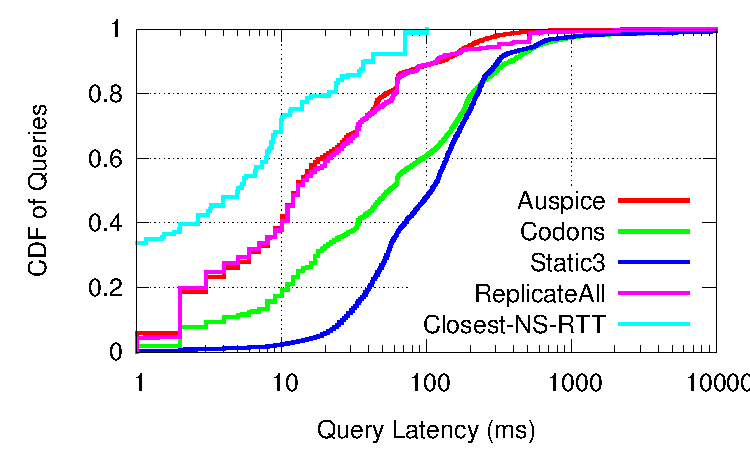
\includegraphics[scale=0.45]{graph/system-exp/cdf-comparison.pdf}}
\subfigure[Median lookup latencies for names.]{\label{fig:namesquerymediancdf}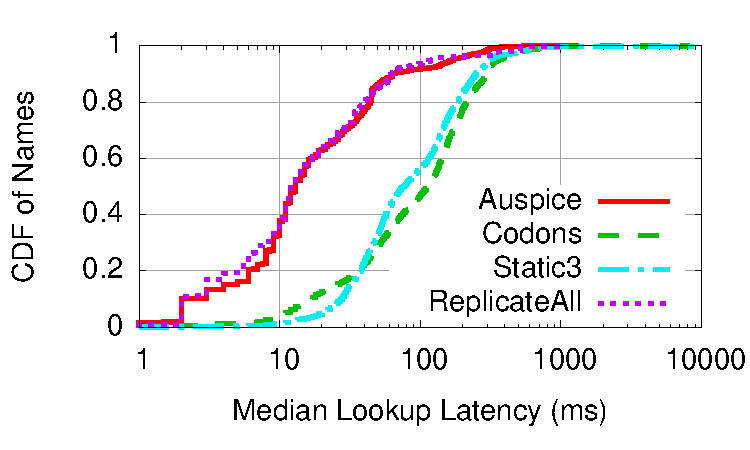
\includegraphics[scale=0.45]{graph/system-exp/cdf-names-median.pdf}}
\subfigure[Update cost of names.]{\label{fig:updatebw}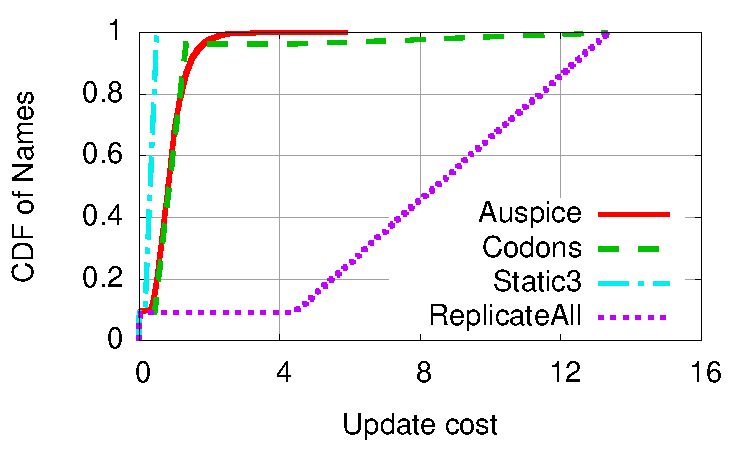
\includegraphics[scale=0.45]{graph/system-exp/cdf-update-cost.pdf}}
\caption{\auspice's lookup latency is nearly equal to \replicateall, yet its median update cost is 10$\times$ less. Locality-unaware schemes, \staticthree\ \& \codons, result in up to 6$\times$ higher median latencies than \auspice.}
\label{fig:lookupupdate}
\end{figure*}


% mobile

We present an evaluation of \auspice\ based on a PlanetLab deployment, cluster-based emulation, and a large scale experiments using our custom simulator. Further, we compare \auspice's performance to today's managed DNS services. 

\begin{itemize}
\item
Locality-aware placement helps \auspice\ achieves nearly 5$\times$ lower latency than a DHT-based replication scheme.
\item
\auspice\ reduces updates costs by nearly an order of magnitude over a replicate-everywhere strategy in a live deployment and yet achieves nearly identical query latencies.
\item
\auspice's load-aware design consistently achieves up to 2 $\times$ lower latencies under a wide range of load scenarios.
\item
With an equal number of name server deployments, \auspice\ achieves comparable DNS lookup latencies to a leading managed DNS provider today, and an DNS update latency which is nearly 2 seconds smaller.
\end{itemize}



%Our evaluation has three main findings. 
%(1) We show that \auspice's strategy of  replicating name records in a locality-aware manner based on read-to-write ratio gives significantly better performance over  locality-unaware replication schemes, including replication schemes implemented over a DHT.
%(2) We show that a global name service can leverage weaker consistency semantics for name records that are updated rarely, including domain names in today's Internet, to significantly reduce user-perceived latency as well as reduce load on the system.
%(3) Mid-session mobility conclusion.


%In this section, we describe our experimental evaluation of \auspice\ on PlanetLab as well as through  trace-driven simulations based on realistic workloads. %We begin with a description of the datasets used to generate workloads.
%Our evaluation has three main goals. 
%First, is to quantify the performance gap between optimal service placement and heuristic service placement strategies in \auspice.
%Second, is to evaluate performance of service placement  schemes in a scenario with high update rates, e.g. a name service for a near future Internet consisting of highly mobile users. 
%Third, is to answer whether service placement decisions considering
%the geo-distribution of users requests improves performance over
%schemes that are agnostic to geo-distribution of users, e.g. \codons. 

%\subsection{Evaluation goals}
%We present an evaluation of the service placement algorithms implemented in \auspice\ on the service workload datasets in Section \ref{sec:datasets}.



\subsection{Replica placement schemes comparison}


In this section, we compare the locality and load-aware replica placement scheme implemented in \auspice\ against alternate replica placement schemes. In line with our goal of designing a name resolution service for mobile hosts in the Internet, we focus on scenarios where a high fraction of name records belong to mobile hosts, with each device updating its network address at high frequency. We conduct experiments with the \auspice\ system comparing replica placement schemes on PlanetLab. For larger scale experiments infeasible on PlanetLab, we present results from a simulator that implements the same replica placement schemes.

%Overall conclusion: Locality-aware scheme does provide a lower latency for a comparable number of replicas, and a comparable load-balance.  (i). \codons's replication achieves poor latency across names. (ii) Naive strategies such as \staticthree\ and \replicateall\ perform worse than schemes that make a controlled number of replicas based on the read to write ratio. (iii) Making controlled number of replicas  based on read-to-write ratio in a locality aware manner provides up to 4$\times$ benefits in terms of latency if those replicas are created randomly.



\subsubsection{Schemes compared}


%\textbf{\locaware} refers to the locality-aware replica placement scheme implemented in \auspice. 

%
\textbf{\codons} is a DNS design implemented on top of Pastry DHT. \codons\ replicates a name record based on its popularity ranking, with more popular name records replicated at greater number of  locations.  The location of replicas is decided by consistent hashing. Our \codons\ implementation retains these features. However, we do not implement multi-hop DHT routing used in \codons. Each request is directly sent to the replica  that would have received this request if Pastry DHT routing were followed.
We achieve this behavior by copying the Pastry routing table of every node at all other nodes and simulating multi-hop routing locally.
Therefore, our latency numbers are a conservative estimate of the latency in \codons. 

\textbf{\staticthree} replicates each name record at three locations that are chosen randomly. \textbf{\replicateall} replicates all name records at all locations. 

\textbf{\opt} uses our optimization formulation (given in Appendix \ref{sec:optimal}) to minimize the total latency including network and server latency.  \opt\ serves as a benchmark for comparison and is implemented only in our simulator. \opt\ is an impractical scheme because solving the optimization problem for billions for name records is well beyond the scope of modern day LP solvers.

%At Internet scale, \opt\ is impractical because of the challenges in solving the optimization problem for billions of name records. 



\subsubsection{Workload}

Our workload consists of lookup requests for name records and updates to them from clients distributed across the globe. In this workload, name records are of two types: \emph{service names} and \emph{device names}. Service names correspond to today's DNS name records, which belong to immobile hosts. Device names correspond to name records for mobile hosts.

Our workload for service names is generated based on traffic statistics for websites reported in Alexa Web Information Service \cite{alexa} (AWIS) dataset. This dataset reports the relative popularity of each website and the geo-distribution of website's popularity at city-level granularity. 
Across different experiments, we generate a workload based on top-1000 and top-10000 most popular websites in this dataset. Today's DNS name records change slowly. Therefore, the number of updates to name records of a service names are less than 1\% of the number of lookup queries in the workload.

%To generate a workload for mobile names, 
%we assume that 

The device names workload exhibits high update rates and a strong geographic locality. The number of updates for a device name are 2-3 orders of magnitude higher than that of a service name. The geo-distribution of requests is as follows: 90\% of requests for a device name originate from 0-5\% of local name servers which are geographically close to each other; remaining 10\% of requests are generated from 5\% local name servers located farther away.

%. \% of requests originate from 0-5\% of local name servers . 

%To generate this workload, every local name server is assumed has an equal number of mobile hosts that send network address updates for their respective device names. 
%Thus,  updates for a mobile name are sent from a single local name server. 
% 90\% of requests for this mobile name are generated from this local name server and up to three  local name servers close to it;  remaining 10\% of queries are generated from 5 local name servers located farther away.

\eat{
The workload for mobile names has two key features. 
First, updates rates for mobile names are much higher than regular names. 
This is because the mobile host that owns a mobile name rapidly changes the set of networks it is connected to. 
Second, requests for a mobile name show strong geo-locality patterns. This is due to several reasons.
Updates for mobile names will originate from the mobile device itself, whose mobility will be contained in a small geographic region for most hosts.
A mobile name will be queried by web services to push updates to the mobile device. Today's web services are geo-replicated to position themselves closer to end-users. Most likely, the closest service replica will query for the mobile name, giving rise to geo-locality.
Another source of a mobile name's queries is communication between two mobile hosts, e.g., a user's friends contacting the user's mobile device to send messages. 
We expect these queries to come from a user's contacts list. Since most of a user's contacts are expected to be within  the same country, these  queries will exhibit strong geo-locality patterns as well.
}



\subsubsection{PlanetLab deployment}

%\begin{minipage}[b]{0.33\linewidth}
%\centering
%\includegraphics[scale=0.45]{newgraphs/pldata1.pdf}
%\caption{Dependence of swarm performance on server bandwidth, and peer arrival rate $\lambda$ for $S$ = 10MB and $\mu$ = 100KBps. Unit of $\lambda$ = sec$^{-1}$.}
%\label{fig:basic}\end{minipage}
%\hspace{0.45cm}

%   \subfigure[$\lambda = 0.45/sec$]{\label{fig:g1-time}\includegraphics[scale=0.34]{newgraphs/target-g1-time.pdf}}




%x	Auspice	Codons	Static3	ReplicateAll	
%Overall-Fairness	0.880849740715	0.983016103853	0.969862385826	0.944348480834	
%Update-Recvd-Fairness	0.923389058562	0.994508958801	0.987580628539	0.943487244312	
%Query-Fairness	0.633390113602	0.780041293236	0.903677640012	0.496513039982	




%
%\begin{figure}
%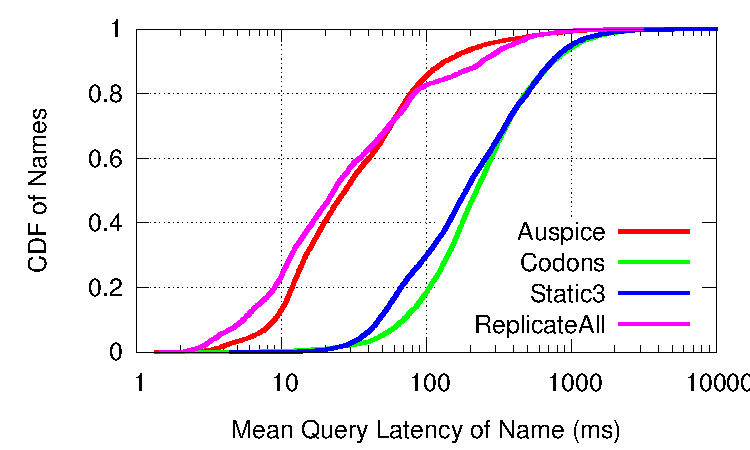
\includegraphics[scale=0.45]{graph/system-exp/cdf-names-mean.pdf}
%\caption{CDF of mean latency of queries for all names.}
%\label{fig:namesquerymeancdf}
%\end{figure}
%
%
%\begin{figure}
%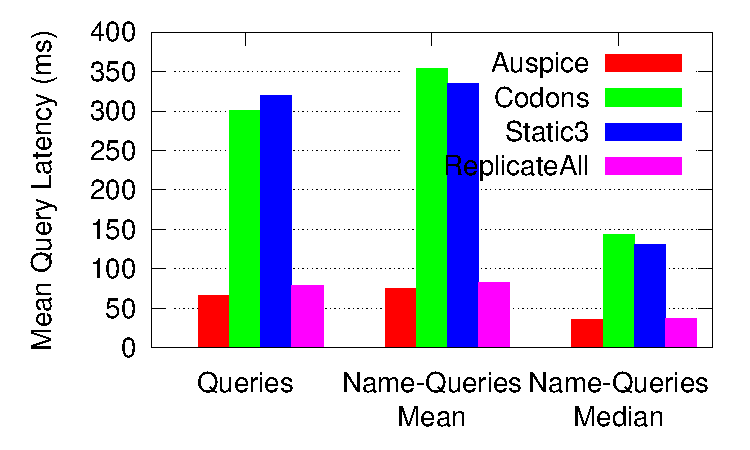
\includegraphics[scale=0.45]{graph/system-exp/mean-latencies.pdf}
%\caption{(1) Mean latency of all queries, (2) Mean of mean latencies of queries for all names, (3) Mean of median latencies of queries for all names}
%\label{fig:meanlatency}
%\end{figure}

%\begin{figure}
%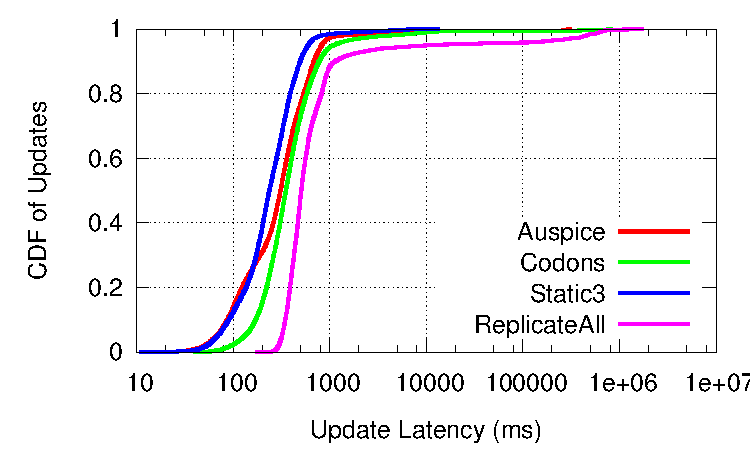
\includegraphics[scale=0.45]{graph/system-exp/cdf-comparison-update.pdf}
%\caption{CDF of  latency of all updates.}
%\label{fig:udpates}
%\end{figure}



%\begin{figure}
%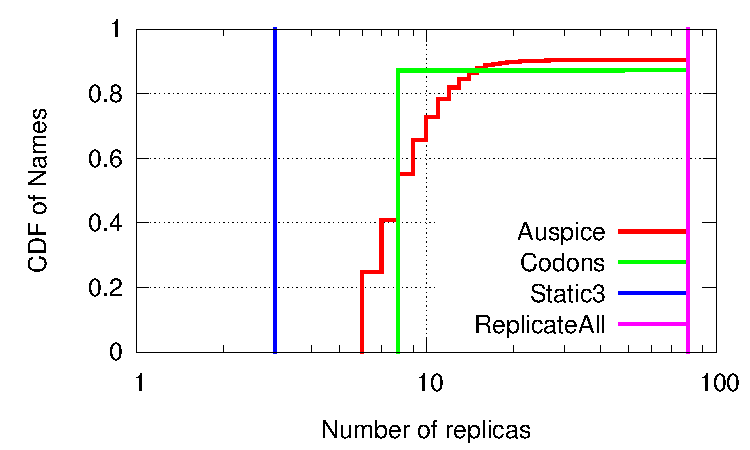
\includegraphics[scale=0.45]{graph/system-exp/cdf-replica-count.pdf}
%\caption{Distribution of the number of replicas for names.}
%\label{fig:cdf-replica}
%\end{figure}






%
%\begin{figure}
%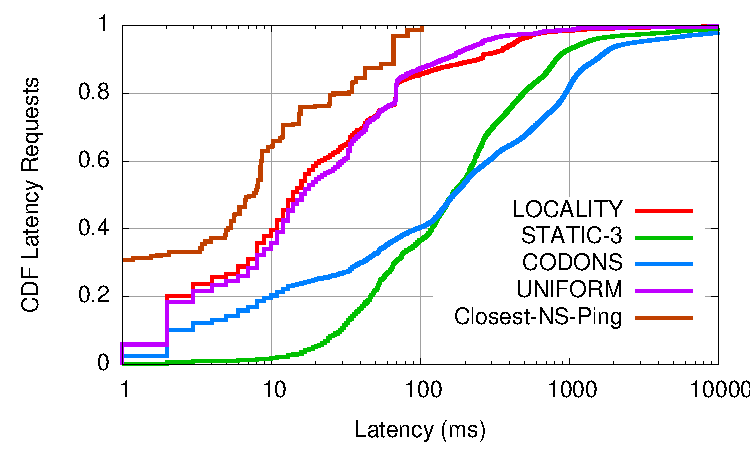
\includegraphics[scale=0.45]{graph/system-exp/high-cdf-comparison.pdf}
%\caption{High load, CDF of latency of all queries. NEW: load balancing, LNS votes for closest NS depending on (network + server) latency. $\alpha$ selected assuming server capacity = 200 req / sec.}
%\label{fig:highquerylatencycdf}
%\end{figure}
%
%\begin{figure}
%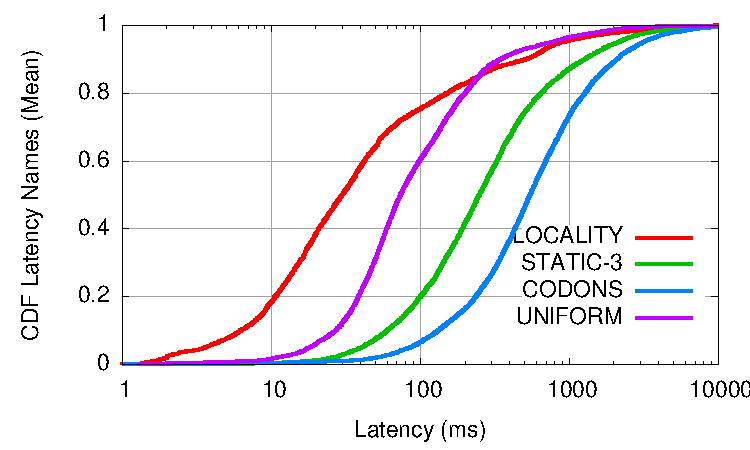
\includegraphics[scale=0.45]{graph/system-exp/high-cdf-names-mean.pdf}
%\caption{High load, CDF of mean latency of queries for all names.}
%\label{fig:highnamesquerymeancdf}
%\end{figure}
%
%\begin{figure}
%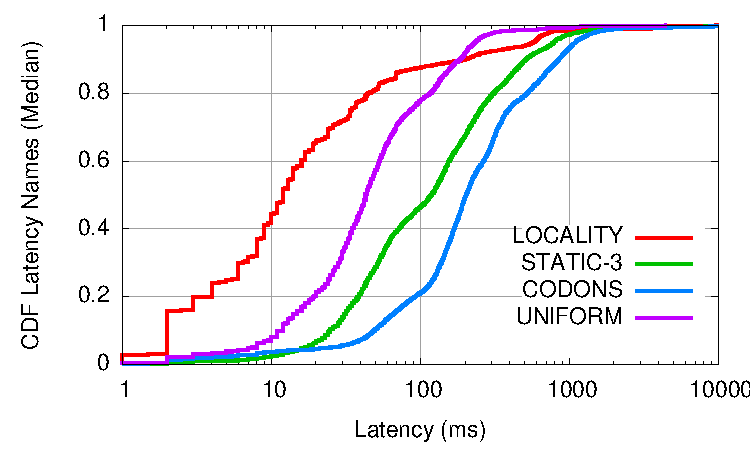
\includegraphics[scale=0.45]{graph/system-exp/high-cdf-names-median.pdf}
%\caption{High load, CDF of median latency of queries for all names.}
%\label{fig:highnamesquerymediancdf}
%\end{figure}



%
%\begin{figure}
%\vspace{1in}
%%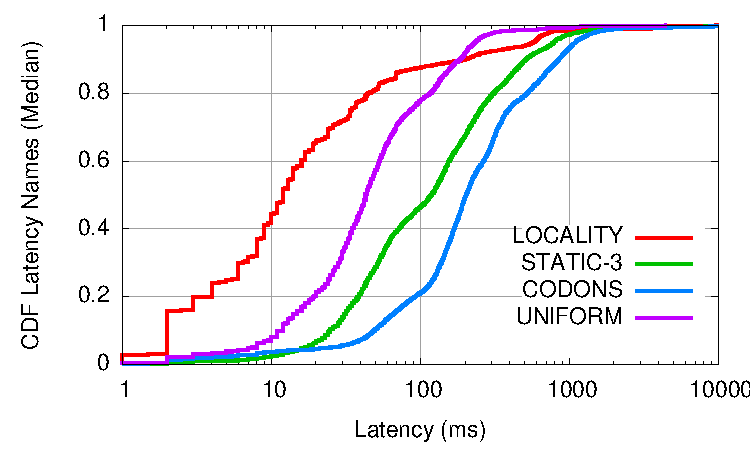
\includegraphics[scale=0.45]{graph/system-exp/high-cdf-names-median.pdf}
%\caption{Latency of \uniform\ as number of replicas is increased compared to the latency of \locaware\ in high load experiments. This graph shows that \uniform\ is not able to outperform \locaware\  even when given the freedom to create unbounded number of replicas. For uniform, increasing the number of replicas starts to increase server latency due to the cost of keeping number of replicas updated.}
%\label{fig:uniform}
%\end{figure}


%\begin{figure}
%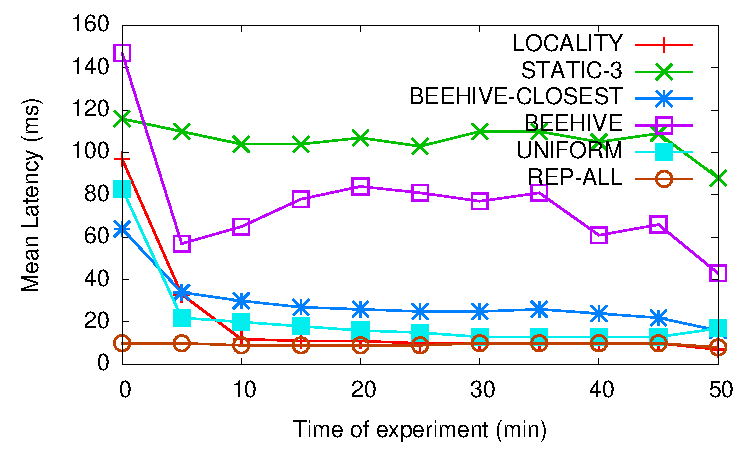
\includegraphics[scale=0.45]{graph/system-exp/timeline-median.pdf}
%\caption{Latency of queries over time. Each point shows the median latency of queries that arrived in the next five minutes.}
%\label{fig:medianlatencytime}
%\end{figure}



Our PlanetLab deployment was done on 160 nodes, 80 nodes running the name server module and 80 nodes running the local name server module. Clients are co-located on the nodes running the local name server module. If PlanetLab nodes are selected randomly, most nodes chosen are either in North America or in Europe.  We use a simple heuristic to select PlanetLab nodes spread across the world. 
For each user-group, the geographically closest local name server location is chosen as its proxy location, e.g., 80 PlanetLab locations  act as a proxy for nearly 15000 cities in the AWIS dataset.


Our workload consists of 4 million lookup requests and 2 million update  requests for  1000 service names and 10000 device names.  Lookup requests are divided equally between service and device names, but almost all updates belong to device names, and only 500 updates are for service names. The requests in the workload are sent over a duration of 30 minutes.


We have configured all schemes to ensure a fair comparison of their replication algorithms. The replication parameter for \locaware\ is calculated assuming each PlanetLab node can serve at least 300 requests / sec with a negligible delay. We have chosen the server capacity somewhat conservatively due to heterogeneity in PlanetLab nodes and because each node is shared among multiple users. 
For the \codons\ scheme, the Zipf exponent is set to $0.63$ calculated based on our workload, and the average hop-count is set to 0.55 which ensures that \codons\ creates nearly the same number of replicas in aggregate as \locaware\ and \uniform.  All schemes use the name server latency estimation implemented in \auspice\  to select the closest replica based on network latency and server latency. An exception is \codons, in which replica selection depends on DHT routing. 

%Figure \ref{fig:cdf-replica} shows the distribution of the number of replicas created by every scheme. 

%\eat{Locality-aware replica placement is configured by setting the replication parameter $\alpha$ = 0.2. This value of $\alpha$ implies that, in this experiment,  a name server will receive 15 requests / sec  on average (as per Equation 14), which clearly is less than the actual capacity of server. Thus we have made a conservative choice in selecting the replication parameter.  A higher alpha value will create more replicas and will likely lower the query latency. The parameters for \codons\ are set to the same values as described in their paper \cite{codons}.}

%We compare replication schemes on four metrics: latency of name record queries (Figure \ref{fig:querylatencycdf}, Figure \ref{fig:namesquerymeancdf}, Figure \ref{fig:namesquerymediancdf}, Figure \ref{fig:meanlatency}),  bandwidth needed to keep name record replicas consistent (Figure \ref{fig:updatebw}), latency of propagating address updates (Figure \ref{fig:udpates}), and a fairness metric to evaluate load balancing property (Figure \ref{fig:fairness-system}). 



%We first compare schemes based on their lookup latencies and update costs 

%We first evaluate schemes on their lookup latency and their update costs Figure \ref{fig:lookupupdate}. Figure \ref{fig:querylatencycdf} shows the CDF of latency of queries of every scheme. A limitation of Figure \ref{fig:querylatencycdf} is that the distribution is biased towards the more popular names in the workload. We expect a global name service to provide low latencies for all names and not just the most popular names. So, we compare the CDF of median  latency of queries for each name in the workload in Figure\ref{fig:namesquerymediancdf}. To evaluate the steady-state performance of all schemes, the latency of initial 25\% of queries are not included in these graphs. 




A locality-aware placement helps \auspice\ to achieve nearly the same lookup latencies as \replicateall, with one-tenth smaller median update cost for a name record than \replicateall. In other words, \auspice\ can match a scheme that uses nearly 10$\times$ as many resources. The \replicateall\ scheme uses 10$\times$ the upload and download bandwidth to propagate updates; it also uses 10$\times$ more server resources to process update messages. A locality-aware design makes efficient use of resources and in scenarios where resources are scarce, it can achieve better performance as well.

%\replicateall\ also adds to server load since every name server must process updates to all name records. In this experiment, PlanetLab nodes indeed have enough server capacity to handle updates to all name records, and therefore server load induced latency is negligible. In a scenario where compute resources are a bottleneck, \replicateall\ could result in poor query latency as is creates due to high server load. 

Locality-unaware schemes such as \staticthree\ and \codons\ cause high latencies. \staticthree\ has a very weak geo-locality of replicas as it chooses three replica locations randomly. While \codons\ create nearly the same total number of replicas as \auspice,  it  answers queries from a replica selected using DHT routing. In many cases, the latency to the selected replica  is higher than the latency to the closest replica for a name record. All other schemes, including \staticthree\ always choose to the closest replica for a name record and hence achieve lower latencies than \codons.  \codons\ replicates 11.2\%   most popular names at all locations. Queries for these names indeed go to the closest replica and achieve low latencies; queries for remaining 88.2\% of names incur high latencies. \codons's design achieves good load balancing under heavy load scenario. In a moderate load scenario, this design results in poor latencies.




\begin{figure}
\centering
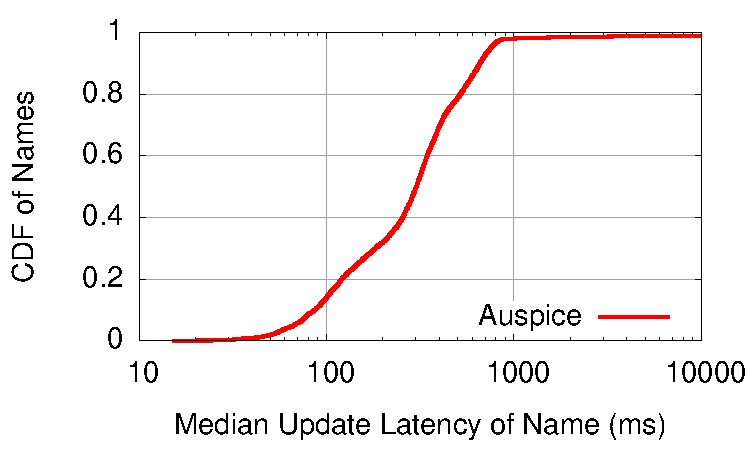
\includegraphics[scale=0.45]{graph/system-exp/cdf-names-median-update.pdf}
\caption{Address update latency of \auspice\ is comparable to other schemes. The high latencies for \replicateall\ are because of insufficient upload capacity on PlanetLab nodes.}
\label{fig:udpates}
\end{figure}

\begin{table}[t]
\centering
\begin{tabular}{ l | c | c}
\hline
Scheme & Update-fairness & Lookup-fairness\\
\hline
\auspice\ & 0.92 & 0.63 \\ 
\hline
\codons\ & 0.99 & 0.74 \\
\hline
\staticthree\ & 0.98 & 0.84 \\
\hline
\replicateall\ & 0.94 & 0.49 \\
\hline
\end{tabular}
\caption{\auspice\ ensures an even distribution of update load among name servers; its lookup fairness is moderately lower due to its locality-aware placement and redirection.}
\label{tab:top10web}
\end{table}


\begin{figure}
\centering
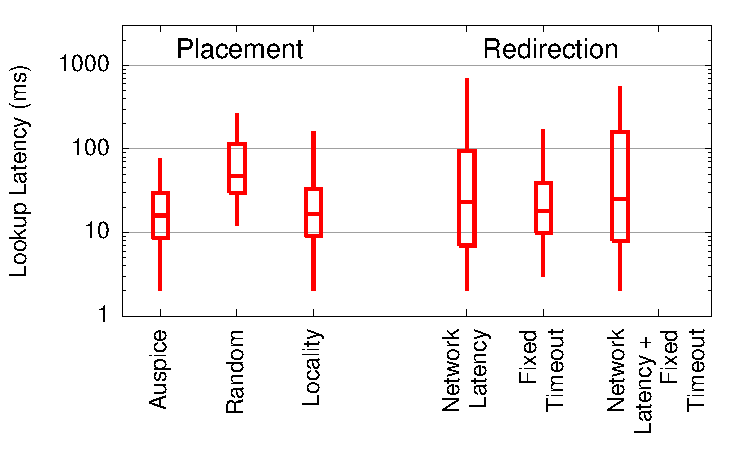
\includegraphics[scale=0.45]{graph/system-exp/mb-stats.pdf}
\caption{Micro benchmarks of \auspice\  show that locality-awareness in the placement phase and load-balancing in the redirection phase are important to achieve good performance.}
\label{fig:micro}
\end{figure}


Address update latency is an important metric for a global naming service . \auspice's address update latencies are of a few hundred milliseconds, and are comparable to that of \staticthree\ and \codons (Figure \ref{fig:udpates}). The \replicateall\ scheme has higher update latencies as it propagates updates to a much greater number of replicas. In our implementation,   an address update is first sent to the Paxos co-ordinator for this name record,  which waits for a confirmation from a majority of replicas, and then replies to the client that the update is complete.  Since the Paxos co-ordinator is chosen randomly among replicas, update latency for all schemes is roughly equal to twice of the round-trip latency between a pair of randomly chosen PlanetLab nodes. This explains why typical update latencies are of a few hundred milliseconds.


The \replicateall\ scheme has median update latencies of 100-1000 seconds for 15\% of names. This is because updates for these names are handled by nodes whose upload capacity is less than that required by \replicateall\ scheme. As a result, updates get queued at name sever and completed updates reflect in the form of high update latencies. 


Do the latency benefits of  a locality-aware placement come at the cost of creating load imbalance at name servers, and how does the load balancing achieved by \locaware\ compare to other schemes? We evaluate the load balancing property in terms of a fairness score \cite{jain-fairness}. The fairness-score is calculated over the number of lookups (updates) received at every name server, and is termed \emph{lookup-fairness} (\emph{update-fairness}). 

All schemes, including \auspice, achieve a  high update-fairness score above ($>$ 0.90), suggesting that update load is balanced evenly across name servers. 
\auspice\ selects replicas based on locality as well as randomly which helps in an even distribution of update load among name servers. 
All schemes achieve a lower score on lookup-fairness ranging between 0.49 (for \replicateall) and 0.84 (for \staticthree). \auspice's achieves a lower lookup-fairness than locality-unaware schemes \staticthree\ and \codons\, but better lookup-fairness of locality-unaware schemes is far outweighed by their poor lookup latencies.

%\locaware\ and \uniform\ have comparable query-fairness suggesting that creating replicas in a locality-aware manner does not significantly hurt the load balancing property. \codons's query-fairness is 33\% higher than that of \locaware, but its better query-fairness is far outweighed by its worse query latency (Figure \ref{fig:namesquerymediancdf}).
%Overall fairness is high despite a lower query-fairness because the number of update messages outnumber queries by at least 3 to 1 for every scheme except static-3.



%For this reason, these nodes could not could not complete all address updates during the experiment. 
%resulting in incorrect network addresses returned to clients. 


%We performed micro-benchmarks  with \auspice\ on PlanetLab to study how each component of its design affects its performance. Each experiments measures \auspice's performance by changing either its resolver placement algorithm or its redirection strategy. Each experiment was repeated three times on three different days and median value is reported. 

Our next experiment presents micro benchmarks for \auspice\ and shows that both its locality-aware placement and its load-aware redirection scheme help to achieve lower latencies. Our micro benchmarks evaluate variants of \auspice's design, and we group our results into two categories, placement and redirection, depending on which aspect of \auspice's design is varied. Figure \ref{fig:micro}  presents our results, and shows mean of the distribution of median latencies of lookups for each name record.

We evaluate two variants of \auspice's placement algorithm, \uniform\ and \locaware. These scheme choose the same number of replicas as \auspice, but \uniform\ chooses all replicas randomly to maximize load balance, and  \locaware\ chooses all replicas based on demand locations.  \auspice\ achieves nearly 4$\times$ lower latencies than \uniform, while the \locaware\ scheme achieves only 20$\%$ higher latencies than \auspice. 
The benefit of a locality-aware placement over a random placement (\uniform) depends on the number of replicas. 
Name records that have a high read-to-write ratio, and are replicated at a large fraction of locations, benefit little from a locality-aware placement. 
Names with a small read-to-write ratio, which are replicated at a small number of locations, achieve a lower latency with a locality-aware placement than a random placement.  In this experiment,  80\% of names are replicated at less than 12 locations, and therefore a locality-aware placement helps. 

%These 80\% of names account for less than 50\% of requests. This explains why the gains of \locaware\ over \uniform\ are greater in  Figure 4 and Figure 5 which compares latency across names, than in Figure 3 which compares latency across requests.


\auspice's redirection strategy has two main components: adaptive timeout and name server latency estimation based on server load and network latency (called load-balancing in short). We evaluate three \auspice\ variants that disable one or both of these features. Instead of using adaptive timeout, we use a fixed timeout value of 150ms which is equal to 95th percentile lookup latency \auspice\ in Figure \ref{fig:querylatencycdf}. Figure \ref{fig:micro} shows that disabling the load-balancing component increases the query latency by nearly 6$\times$. Load-balacing helps identify a few PlanetLab server that are experiencing high load which significantly reduces mean query latencies. A fixed timeout of 150 ms gives higher latencies than an adaptive timeout values. While it is possible to choose a fixed timeout value more carefully, adaptive timeout provides good performance and does not require parameter tuning.








%\locaware\ achieves nearly the same lookup latency as \replicateall\  but 

%\locaware\   and \replicateall\ both achieve the least query latency among all schemes, 
%but \replicateall\ scheme consumes nearly 9$\times$ more download bandwidth at a typical node than \locaware\ to keep name records consistent (Figure \ref{fig:updatebw}).
%\replicateall\ consumes an equally high upload bandwidth at a typical node to push address updates to all other name servers  (graph omitted for brevity). 
%

%To validate this claim, we performed a experiment on a cluster environment with gigabit-capacity network links. The aggregate update rate was nearly 3$\times$ higher than in the PlanetLab experiments. In this case, \replicateall\ scheme resulted in a worse query latency than  \staticthree\ and \locaware.





%\locaware\ creates the nearly same number of replicas as \uniform\ for every name (Figure \ref{fig:cdf-replica}), but it creates them close to the pockets of demand resulting in a lower query latency.


%The benefit of locality-aware placement is greater for mobile names than for regular names.

%Regular names have a high ratio of (read rate) / (write rate), hence both \uniform\ and \locaware\ create a large number of replicas of regular names. 
%For this reason, locality-aware placement of replicas provides less benefits to \locaware\ over \uniform\ for queries belonging to regular names, that constitute 86\% of all queries.
%The (read rate) / (write rate) ratio of mobile names is less than 1, hence only one active replica is created for mobile names. The \locaware\ scheme achieves a lower query latency than \uniform\ by placing an active replica in a locality-aware manner. Since 89\% of names are mobile names, this also explains why \locaware\ shows high gains over \uniform\ when CDFs across names are compared.


%\replicateall\ strategy is wasteful of network and server resources, and \locaware\ scheme achieves the same query latency while using much less resources.  



% comparison of locality and replicate all
%\eat{The \replicateall\ scheme does achieve a lower latency than \locaware\ but \replicateall\ creates 7.15$\times$ more replicas than \locaware\ or \uniform\ in this experiment. \replicateall\ is not a practical scheme for a global name service because each node must handle all updates. The aggregate update rate of a global name service  will exceed the capacity of a single node which will result in poor performance. To validate this claim, we performed a experiment on a cluster environment with an aggregate update rate of 2750 req/sec in which \replicateall\ scheme resulted in a worse query latency than  \staticthree\ and \locaware.}




%\subsubsection{Throughput under high load}

%In this experiment, we have shown that replicating name records in a locality-aware manner based on the read-to-write ratio gives the best performance. The experiments with our \auspice\ prototype were conducted on a  smaller scale workload than a global name service is expected to handle and and our server deployment was restricted by the number of reliable geo-distributed PlanetLab servers we could obtain. Therefore, we next present experiments from our simulator that that compares replication schemes for a larger server deployment and workload sizes.

\subsubsection{Simulator}



One question to discuss. How do replication schemes compare at low-load (0-10\%), moderate-load (50\%)and high-load (90\%) scenarios. In the system experiment, the locality-benefits of \locaware\ outweigh the load-balancing benefits of \uniform\ and \codons. When this load increases, is there a regime where load balancing benefits of \uniform\ and \codons\ enable them to outperform a locality-aware replication scheme? 


\subsection{Comparison to managed DNS services}


%\subsection{Benefits of high TTL}

%\begin{figure}
%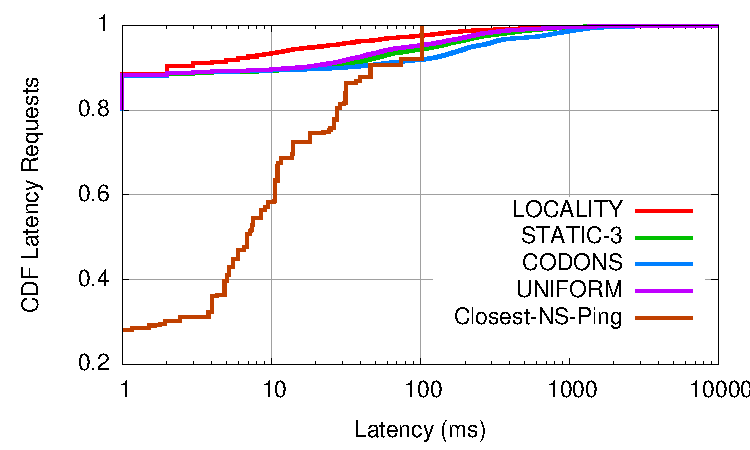
\includegraphics[scale=0.45]{graph/system-exp/ttl-cdf-comparison.pdf}
%\caption{High TTL, high load, CDF of latency of all queries. TTL are set comparable to the write rates of regular names. TTL are set comparable to be write rates of regular names.}
%\label{fig:ttlquerycdf}
%\end{figure}
%\begin{figure}
%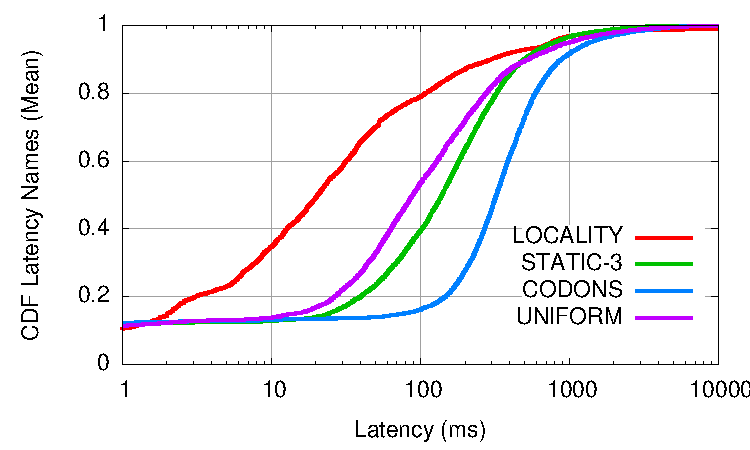
\includegraphics[scale=0.45]{graph/system-exp/ttl-cdf-names-mean.pdf}
%\caption{High TTL, high load, CDF of mean latency of queries for all names.}
%\label{fig:ttlnamesmean}
%\end{figure}
%\begin{figure}
%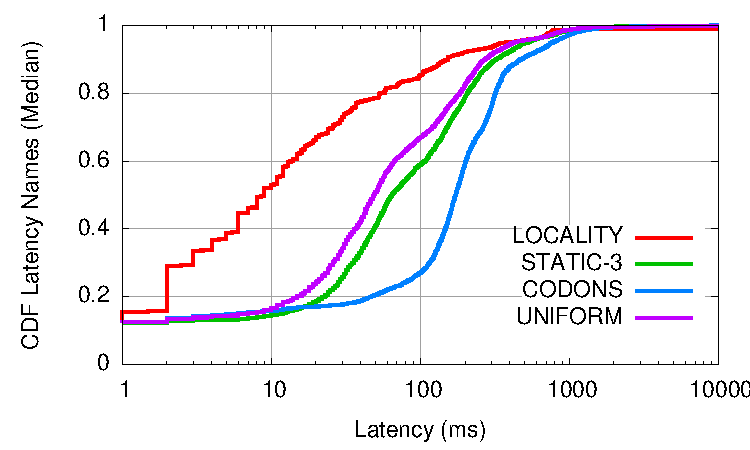
\includegraphics[scale=0.45]{graph/system-exp/ttl-cdf-names-median.pdf}
%\caption{High TTLs, high load, CDF of median latency of queries for all names.}
%\label{fig:ttlnamesmedian}
%\end{figure}

%High TTLs can significantly lower the latency for regular names queries. 



%\begin{figure}
%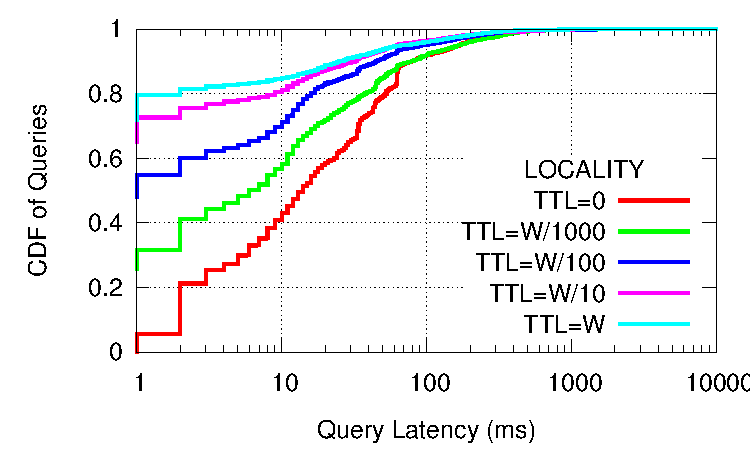
\includegraphics[scale=0.45]{graph/system-exp/ttl-cdf.pdf}
%\caption{W = average interval between change of network address for regular names. A TTL-value equal to W/10 provides considerable reduction in latency over a TTL-value of zero or the using a TTL-value 100-1000$\times$ smaller than W.}
%\label{fig:ttlvary}
%\end{figure}

%\begin{figure}
%\vspace{1.5in}
%\caption{This graph shows the latency CDF across names for \locaware\ when TTLs are set to 0.01\%, 0.1\%, 1.0\%, 10.0\% of write rate for mobile names. High TTLs reduce the load on the system resulting in improved latency for mobile names as well.}
%\label{fig:ttlvarynames}
%\end{figure}



%(2) Codons scheme performs well for names it replicates every where, for other names in most cases it performance is worse than Static-3 which replicates names. Focus on load balancing results in poor latencies. If we compare latency across names, its performance is the worst.

%(3) The difference between Uniform and Locality shows the value of placing replicas in a locality-aware manner.

%(4) Compare the number of replicas: locality creates less replicas than beehive and  uniform scheme. 

%
%
%Write performance: 
%
%Write latencies are comparable. 




%\subsubsection{Simulator}


%\subsection{Comparison to DNS}
%This section compares \auspice\ to today's DNS. Through distributed measurements on PlanetLab testbed.


\subsection{Mid-session mobility}


%\input{eval2}
%!TEX root = shrink.tex
\section{Experimental Evaluation}
\label{sec:shrink-eval}
\newcommand{\peakS}{Peak-S}
\newcommand{\peakSN}{Peak-SN}
\newcommand{\randSN}{Rand-SN}

Our evaluation has two main goals: (1) Comparing the network energy use of \shrink\ against a network-unaware server consolidation scheme (Section \ref{sec:net-compare}). (2) Quantifying the energy-response time tradeoff achieved by \shrink\ and compare it to the ideal energy response time tradeoff achievable (Section \ref{sec:quantify}).

\begin{figure}[t]
        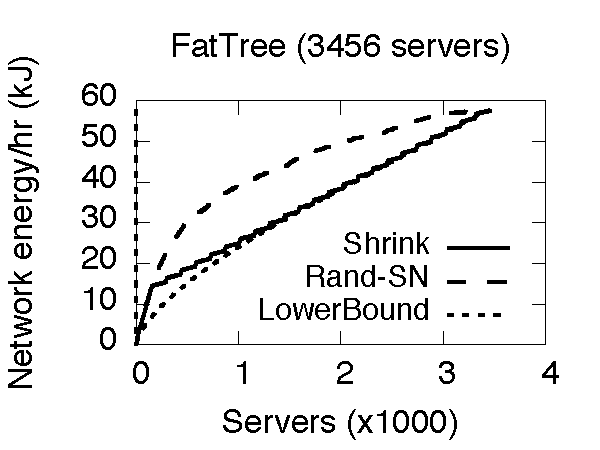
\includegraphics[scale=0.4]{graphs/final/fattree-24.pdf}
                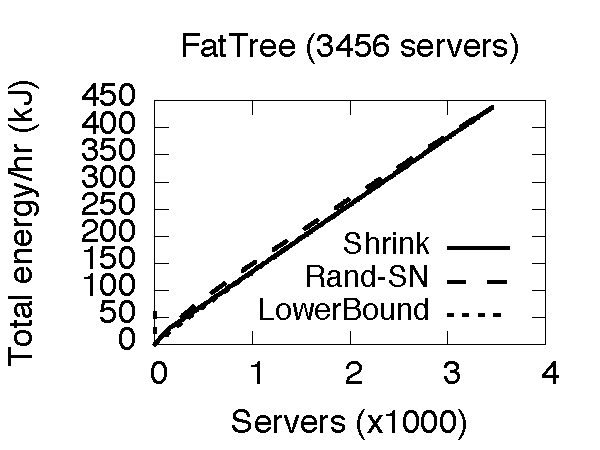
\includegraphics[scale=0.4]{graphs/final/fattree-24-total.pdf}
                        \centering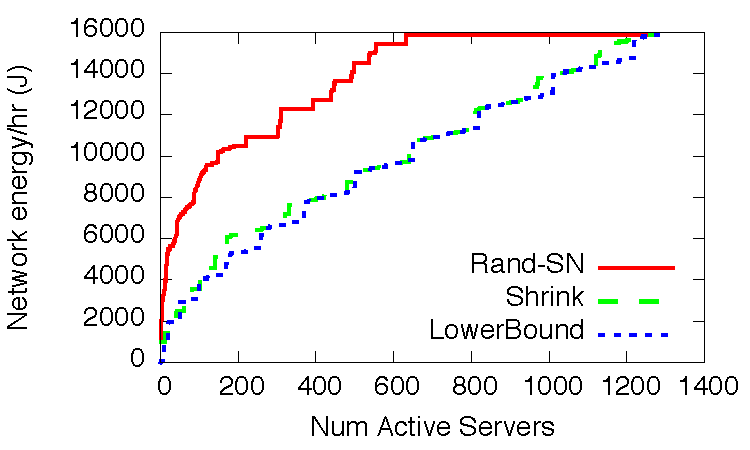
\includegraphics[scale=0.4]{graphs/final/vl2.pdf}
                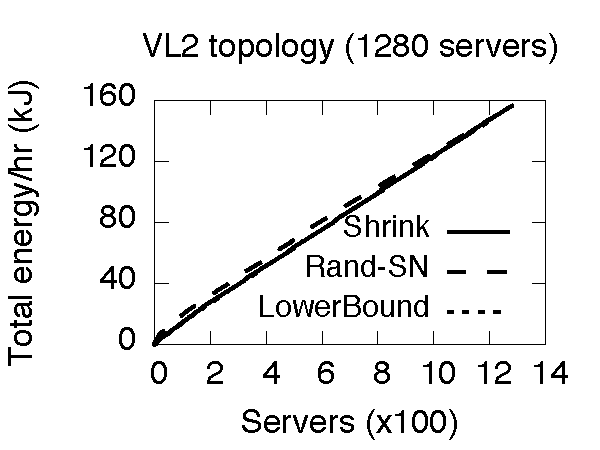
\includegraphics[scale=0.4]{graphs/final/vl2-total.pdf}
\caption{[Numerical computation] \shrink's network energy use is lower than a network-unaware server consolidation scheme \randSN\ by 38\% on FatTree and 42\% on VL2 when one-fourth of the servers are active in each topology.}
\label{fig:fattree}
\end{figure}

\subsection{Comparing network energy use}
\label{sec:net-compare}

\textbf{Schemes compared:}   (1) \emph{\randSN:} \randSN\ selects the set of active servers randomly; it uses the same network consolidation scheme as \shrink.  \randSN\ is used to evaluate the benefit of network-aware server consolidation in \shrink. (2) \emph{LowerBound:} We define lower bounds on the network energy use for a given number of active servers on the FatTree and the VL2 topologies. Our computation of LowerBound for FatTree and VL2 is described in Appendix \ref{sec:netlb}. \randSN\ and LowerBound provide the same per-server bandwidth guarantee to external hosts as \shrink\ does.

\textbf{Topologies:}  We simulate two network topologies:  a 3456-server FatTree topology made of 24-port switches (Cisco Nexus 2224P, 80 Watt, 720 count) \cite{cisco-dc-switches} consuming 80 Watt per switch, and a 1280-server VL2 topology made of 24-port ToR switches (Cisco Nexus 2224P, 80 W, 64 count) \cite{cisco-dc-switches} and 16-port 10 Gigabit core or aggregation switches (Cisco Catalyst 6500, 480 W, 24 count) \cite{catalyst-6500}. We assume all active servers have identical power use (Acer Altos T350 F2, 130W at 60\% utilization \cite{spec}).

\textbf{Results:}  Figure \ref{fig:fattree} presents our results.
%compares \shrink\ against \randSN\ and the lower bounds on network energy use for the simulated topologies.
The relative difference between \shrink\ and \randSN\ reduces as the number of active servers increases. 
When 25\% and 50\% of servers are active, \shrink's network energy use is lower than \randSN\ by 38\% and 26\% respectively on FatTree and 42\% and 35\% respectively on VL2. 
When 25\% and 50\% of servers are active, \shrink's network energy use higher than LowerBound by 9\% and 2\% respectively on FatTree and by 13\% and 7\% respectively on VL2. 
These findings show that \shrink's network-aware server consolidation reduces the network energy use over network-unaware server consolidation schemes and gives network energy savings close to the lower bound.
When 25\% and 50\% of servers are active, \shrink's \emph{total} energy use is lower than \randSN\ by 9\% and 5\% respectively on FatTree and 10\% and 7\% respectively on VL2. 
Thus, \shrink's network-aware server consolidation is effective in reducing aggregate \cdc\ energy use as well. 

%Considering scenarios where at least one-fifth of servers are active, \shrink\ uses up to 39\% less network energy on FatTree and up to 45\% less energy on VL2 compared to the network-unaware scheme, \randSN. 


\begin{figure*}
        \centering
        \subfigure[Mean]{\label{fig:pe-mean}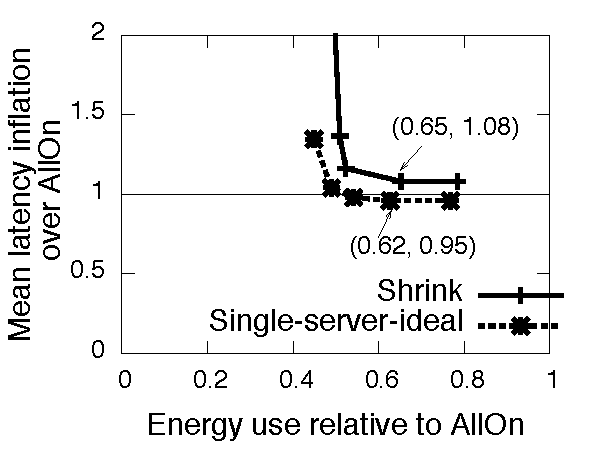
\includegraphics[scale=0.47]{graphs/final/mean.pdf}}
         \subfigure[95-th percentile]{\label{fig:pe-95}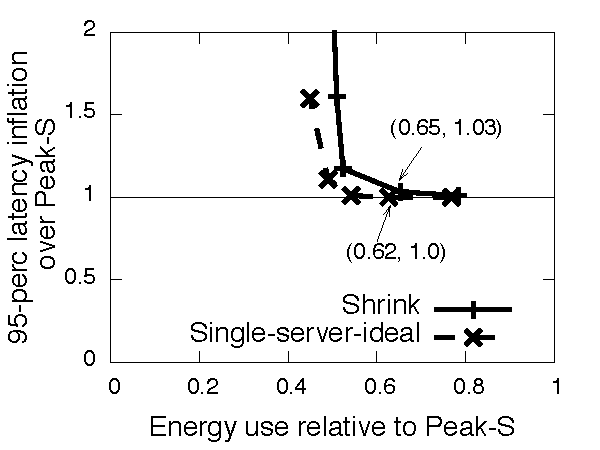
\includegraphics[scale=0.47]{graphs/final/perc95.pdf}}	       \subfigure[99-th percentile]{\label{fig:pe-99}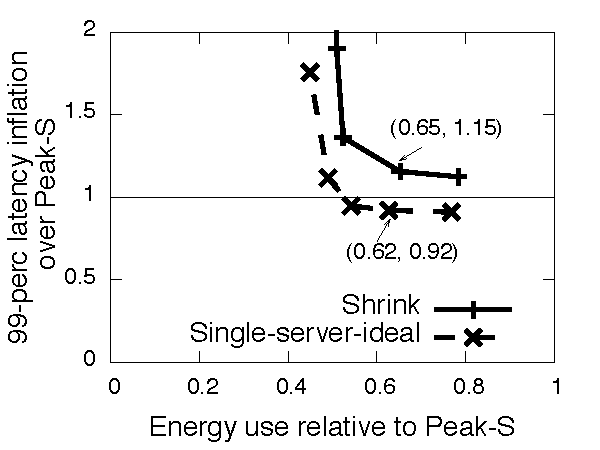
\includegraphics[scale=0.47]{graphs/final/perc99.pdf}}	
        \caption{Server consolidation (Section \ref{sec:ec2}):  \shrink's reduces energy over \peakS\ with a small response time inflation. In Figure \ref{fig:pe-mean}, \shrink's energy use is 0.65$\times$ of \peakS\ and its mean response time is 1.08$\times$ of \peakS; Single-server-ideal's energy use is 0.62$\times$  of \peakS\ and its mean response time is 0.95$\times$ of \peakS.}
        \label{fig:pe}
\end{figure*}

\subsection{Quantifying energy-response time tradeoff}
\label{sec:quantify}
\vspace{-0.1in}
\subsubsection{Experiment setup}
\label{sec:setup}
\textbf{Akamai dataset:} Our evaluation uses content access traces from an Akamai datacenter. The traces include all requests received at a datacenter with 24 servers for a week in December 2013. We restricted our data collection to a small datacenter as we did not have the resources to experiment with traces from a significantly larger datacenter. Our anonymized traces include several major types of traffic observed in a CDN such as video, social media and other web traffic. Each anonymized log entry includes among other fields, the request timestamp, content URL, size of requested content, actual number of bytes sent and IP address of the user. Overall, the traces contain more than 2 billion requests generating nearly 200 TB of network traffic.

\textbf{Testbeds:} We use prototype-based experiments (on EC2 and Emulab) and trace-based experiments. Our experiment on EC2 evaluates the energy-response time tradeoff due to server-only consolidation. As we do not have control over network topology on EC2, we use Emulab to evaluate the response time inflation due to both server and network consolidation. Finally, we conduct larger-scale trace-based experiments on a simulator.






%\begin{figure}[t]
%        \centering
%        \begin{subfigure}{0.24\textwidth}
%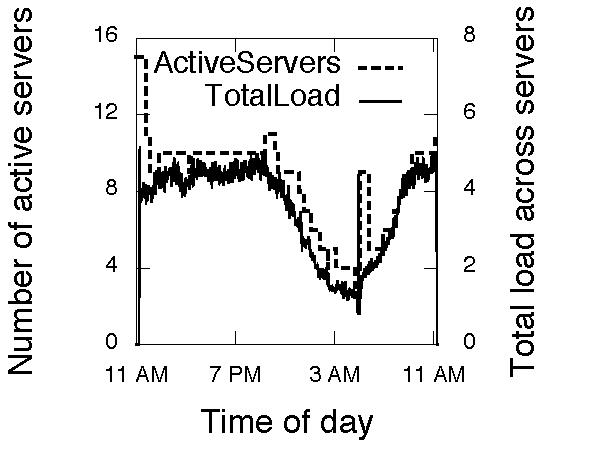
\includegraphics[scale=0.4]{graphs/final/num-servers.pdf}
%\caption{}
%\label{fig:num-servers}
%        \end{subfigure}
%        \begin{subfigure}{0.24\textwidth}
%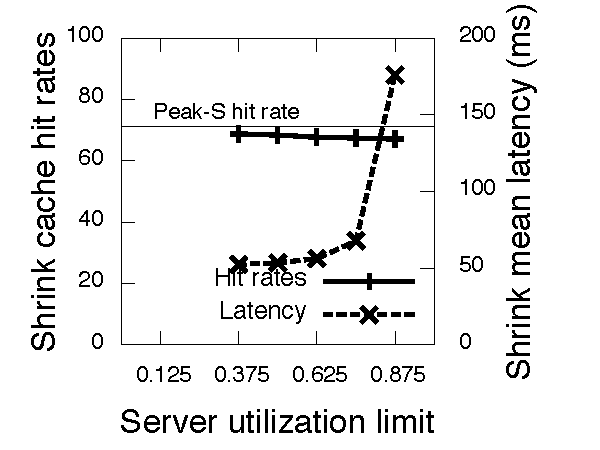
\includegraphics[scale=0.4]{graphs/final/hit-rate.pdf}
%\caption{}
%\label{fig:hitrate}
%        \end{subfigure}
%        \caption{[EC2] \shrink\ adapts the number of active servers based on \cdc\  load to reduce energy over \peakS. Cache hit rates and mean response time for \shrink\ and \peakS.}
%\end{figure}


%\centering
%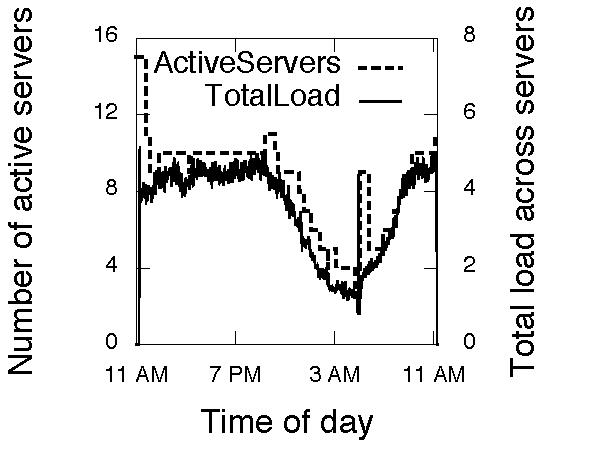
\includegraphics[scale=0.6]{graphs/final/num-servers.pdf}
%\caption{[EC2] \shrink\ adapts the number of active servers based on \cdc\  load to reduce energy over \peakS.}
%\label{fig:num-servers}
%\end{minipage}
%\hspace{0.5cm}
%\begin{minipage}{0.3\textwidth}
%\centering
%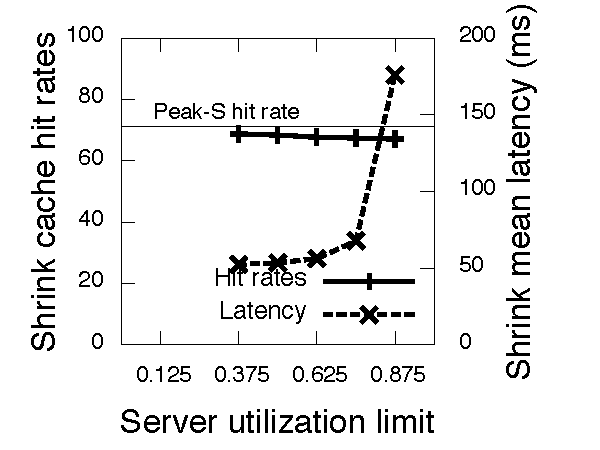
\includegraphics[scale=0.6]{graphs/final/hit-rate.pdf}
%\caption{[EC2] Cache hit rates and mean response time for \shrink\ and \peakS.}
%\label{fig:hitrate}
%\end{minipage}
%\hspace{0.5cm}
%\begin{minipage}{0.3\textwidth}
%\centering
%	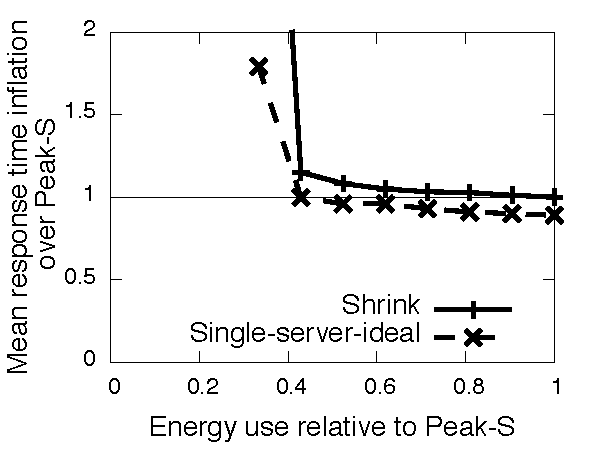
\includegraphics[scale=0.55]{graphs/final/emulab-mean.pdf}
%	\caption{[Emulab] Network and server consolidation: For an 15\% increase in mean response time, \shrink\ reduces energy use by 57\% over \peakS.}
%	\label{fig:pe-mean-2}
%
%\end{minipage}
%\end{figure*}

%
%\begin{figure*}
%\begin{minipage}{0.3\textwidth}
%\centering
%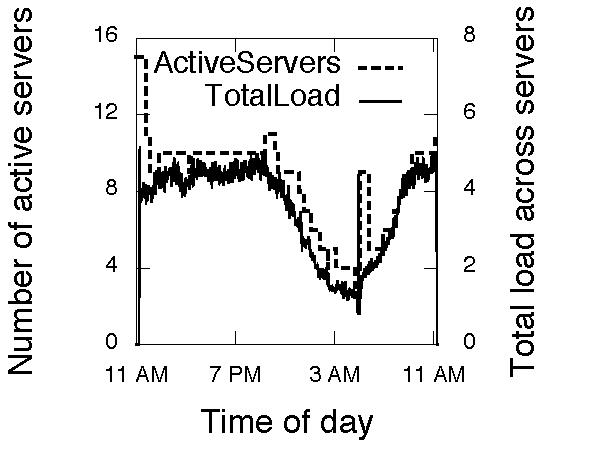
\includegraphics[scale=0.6]{graphs/final/num-servers.pdf}
%\caption{[EC2] \shrink\ adapts the number of active servers based on \cdc\  load to reduce energy over \peakS.}
%\label{fig:num-servers}
%\end{minipage}
%\hspace{0.5cm}
%\begin{minipage}{0.3\textwidth}
%\centering
%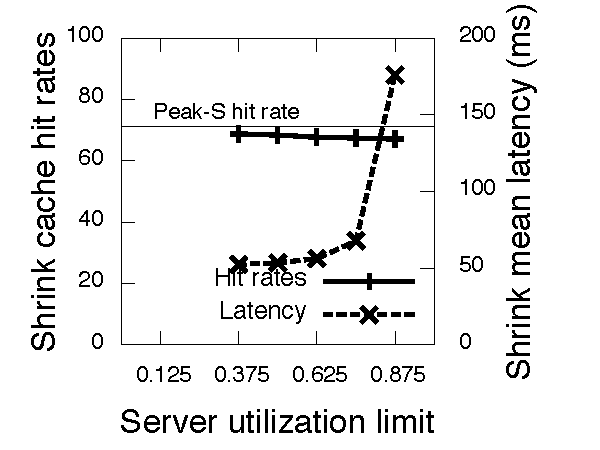
\includegraphics[scale=0.6]{graphs/final/hit-rate.pdf}
%\caption{[EC2] Cache hit rates and mean response time for \shrink\ and \peakS.}
%\label{fig:hitrate}
%\end{minipage}
%\hspace{0.5cm}
%\begin{minipage}{0.3\textwidth}
%\centering
%	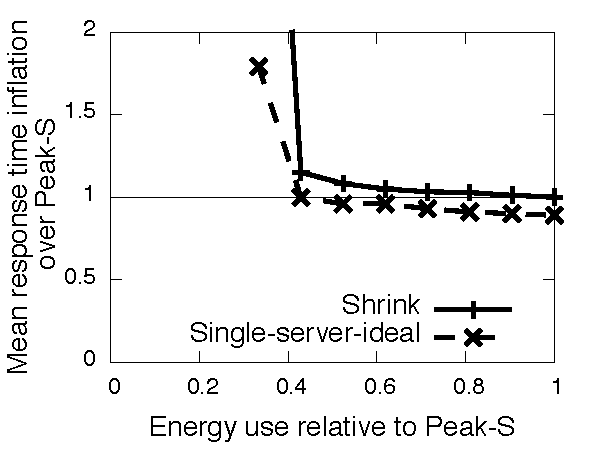
\includegraphics[scale=0.55]{graphs/final/emulab-mean.pdf}
%	\caption{[Emulab] Network and server consolidation: For an 15\% increase in mean response time, \shrink\ reduces energy use by 57\% over \peakS.}
%	\label{fig:pe-mean-2}
%
%\end{minipage}
%\end{figure*}


\textbf{Schemes compared:} We compare \shrink\ against \emph{\peakS} and \emph{Single-server-ideal}. \peakS\ represents a baseline in which a \cdc\ operator does not use consolidation to reduce energy use, i.e., it keeps all servers and switches active.

Single-server-ideal is a computation of the ideal energy-response time curve, unachievable by any real system. The points on this curve are obtained by varying the utilization $u$ up to which any server can be loaded. For a given $u$, the response time of Single-server-ideal for a given metric is equal to the measured load-vs.-response time curve of a single server for the same metric at the same utilization. For the same utilization $u$, any distributed system will have a higher response time because workload dynamics, load imbalance and non-steady state cache behavior; these factors are ignored by Single-server-ideal. Our single server measurements are done with a representative workload in the respective experimental environment, EC2 or Emulab, with emulated client-to-server delay and server-to-origin delay. 

%taken to be response of a single server in steady-state at the same utilization. In doing so, we assume that the response time of the entire \cdc\ at a given average utilization is the same as that of a single server  at the same utilization. 

For Single-server-ideal, we compute the set of servers and switches in each time interval that minimizes the total energy use as follows. Based on four inputs -- $u$, the total load in each time interval, the number of server transitions allowed, and the power model of each server --, we use a dynamic programming algorithm to compute the total energy use of servers and the number of active servers in each time interval. The number of transitions is equal to one on-off server transition/server/day or the same number of transitions as \shrink\ in that experiment, whichever is higher. The ideal network energy use for the tree topology we experiment with (Section \ref{sec:emulab}) is computed based on the number of active servers in each time interval. The set of active servers are selected in a left-to-right order; for each active server, we select the switches on the path to the root. The set of switches selected across all active servers is the set that optimizes network energy use.

%Single-server-ideal is a computation of the ideal energy-response time curve. In our computation, we assume that the utilization-vs.-response time curve for the entire \cdc\  is the same as that of a single server system at the same utilization, which is in steady state and has an infinite cache. 
%The response time of Single-server-ideal is \emph{ideal}, as discussed in Section \ref{sec:analysis}. For our computation, we obtained the utilization-vs.-response time curve for a single server by measuring response time metrics at varying request rates and using a cache size large enough so that steady state response times can be measured without exhausting the cache.
%
%The energy calculation for Single-server-ideal assumes prior knowledge of the total load in each time interval and the number of server transitions allowed. We allow Single-server-ideal to make one on-off server transition/server/day or the same number of transitions as \shrink\ in that experiment, whichever is higher. Based on these inputs, we use a dynamic programming algorithm \cite{mathew12} to compute the total energy use of servers and the number of active servers in each time interval.  The network energy use for the tree topology we experiment with (Section \ref{sec:emulab}) is computed as follows: For each active server, we select the switches on the path to the root. The set of switches selected across all active servers is the set that optimizes network energy use.



\subsubsection{Prototype-based experiments: server consolidation}
\label{sec:ec2}
\vspace{-0.1in}
This experiment quantifies the energy-response time tradeoff due to server consolidation on EC2. Our EC2 testbed consists of 15 servers, 15 clients and 4 origin servers running on independent m3.xlarge instances (4 core, 15 GB RAM, 40 GB$\times$2 SSD), all in the same datacenter. Our origin server is a trivial Apache Tomcat application that dynamically generates the requested content. We emulate a 60 ms RTT between origin servers and \cdc's servers, and a 10 ms RTT between client and server machines. We configured each server to use an 8 GB memory cache and a 30 GB cache on each SSD. 

Our workload consists of a 24-hour duration of the trace.  We selected one-eighth of the content randomly from the trace but sped up the trace by 8$\times$ to send those requests over a 3-hour duration. Thus, we  maintain approximately the same load on the servers. We use a short pre-shutdown wait interval $W =$ 10 min for \shrink\ because our workload is a sped up by $8\times$.

%
We calculate the energy savings relative to \peakS\ as per Equation \ref{eq:benefit}; the ratio of the idle to peak energy use of servers, $I$ equals 0.5 \cite{barroso2007case}. \peakS\ uses 15 servers in this experiment. We have conservatively chosen the number of servers in \peakS\ to be much less than the number of servers in the Akamai datacenter itself so as not to overestimate the energy savings. 



We evaluate \shrink\ in terms of three response time metrics --  mean, 95-percentile, 99-percentile. 
To provide a utilization-vs.-response time curve $F(.)$ to \shrink\ for each metric, we take the first approach discussed in Section \ref{sec:utilization-vs-responsetime}. The function $F(.)$ for each metric is equal to the measured utilization vs. response time curve of a single server with an inefficiency factor $\rho = 0.2$.  Based on $F(.)$ for each metric, we specify response times $F(u)$ to \shrink\ for values of $u$ from 0.375 to 0.875 at intervals of 0.125 across different runs. 

%, which is much less than the number of servers in the Akamai datacenter itself. we have made this choice not to overstate the energy savings.


Figure \ref{fig:pe} compares the response time and the energy use of \shrink\ relative to \peakS\ for the mean, the 95-th percentile and the 99-th percentile of response times. \shrink\ reduces energy use by 35\% over \peakS\ while inflating the mean, the 95-th percentile and the 99-th percentile by 8\%, 3\% and 15\% respectively. 
To explain the difference between \peakS\ and \shrink, consider Figure \ref{fig:ec2-other} (left)  which shows the aggregate load and the number of servers from one of the runs of the system. \shrink\  adapts the number of active servers based on load in the system keeping only 3 servers active when the load is the lowest, but \peakS\ always keeps 15 servers active and hence has a higher energy use. This result implies that an operator for which these inflations are tolerable, e.g., they do not cause an SLA violation, can achieve the corresponding energy savings as well. 




%Single-server-ideal does achieve a better energy-response time tradeoff than \shrink.  First, the energy-response time curve for Single-server-ideal is computed assuming that the response time for a given server utilization limit is equal to the response time of a single server in steady state at the same utilization. The response time for any real system, including \shrink, will be higher due to several reasons such as imperfect load balancing and non-steady state cache behavior. 




Does  an increase server load or a decrease in cache hit rates cause a greater impact on \shrink's response time over \peakS? 
In Figure \ref{fig:ec2-other} (right) the x-axis shows the server utilization limit $U$ computed by \shrink's consolidation algorithm (Section \ref{sec:serverconsolidation}) and y-axes show corresponding the  hit rates and the mean response time of \shrink. \shrink's  hit rates are lower than \peakS\ but the decrease is less than 7\% across all utilizations. 
Thus, the response time inflation due to a decrease in hit rates is likely to be small. A small reduction in hit rates is not surprising given that the Zipf exponent for the Akamai trace is 0.8 as per our calculations, and our model in Section \ref{sec:analysis} has suggested that  consolidation reduces hit rates by a small fraction for for real workloads with a high skew in content popularity.  We find that mean response times increase sharply at  a high server utilization limit, e.g. $U=0.875$, which is likely due to an increase in server load. To summarize, there is a small response time inflation due to a decrease in hit rates but severe inflation occurs at high server utilization limits, and is likely due to an increase in server  load.


Comparing \shrink\ with Single-server-ideal, in Figure \ref{fig:pe-mean}, \shrink's energy use is 0.65$\times$ of \peakS\ and its mean response time is 1.08$\times$ of \peakS; Single-server-ideal's energy use is 0.62$\times$  of \peakS\ and its mean response time is 0.95$\times$ of \peakS.  
There are two reasons that explain the gap between \shrink\ and Single-server-ideal. First, Single-server-ideal ignores several factors that increase response time of any distributed system such as workload dynamics, load imbalance and non-steady state cache behavior. Second, \shrink\ waits for the pre-shutdown wait interval to see if a decrease in load persists before turning servers off. But, in our calculation, Single-server-ideal knows the load for the entire experiment beforehand and hence it can shutdown servers sooner than \shrink\ and save more energy.

%An implication of our findings is that a simple random load balancing policy effectively avoids load hotspots and ensures only a small decrease in cache hit rates even as energy optimization schemes vary the number of active servers in a \cdc.
\begin{figure}
\centering
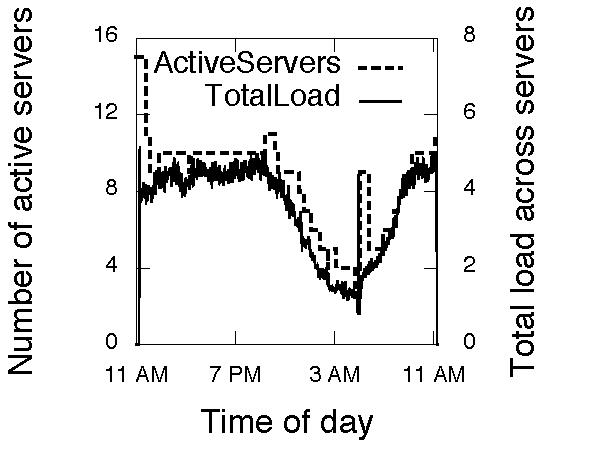
\includegraphics[scale=0.4]{graphs/final/num-servers.pdf}
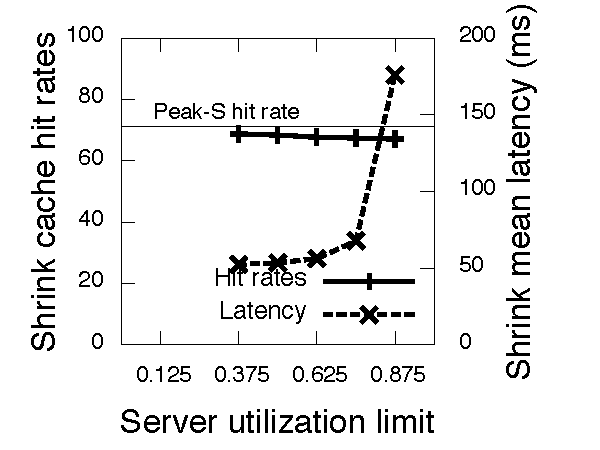
\includegraphics[scale=0.4]{graphs/final/hit-rate.pdf}
\caption{Server consolidation (Section \ref{sec:ec2}): [Left] \shrink\ adapts the number of active servers based on \cdc\  load to reduce energy over \peakS. [Right] Cache hit rates and mean response time for \shrink\ and \peakS.}
\label{fig:ec2-other}
\end{figure}

\subsubsection{Prototype-based experiments: server \& network consolidation}
\label{sec:emulab}

\begin{figure}
	\centering
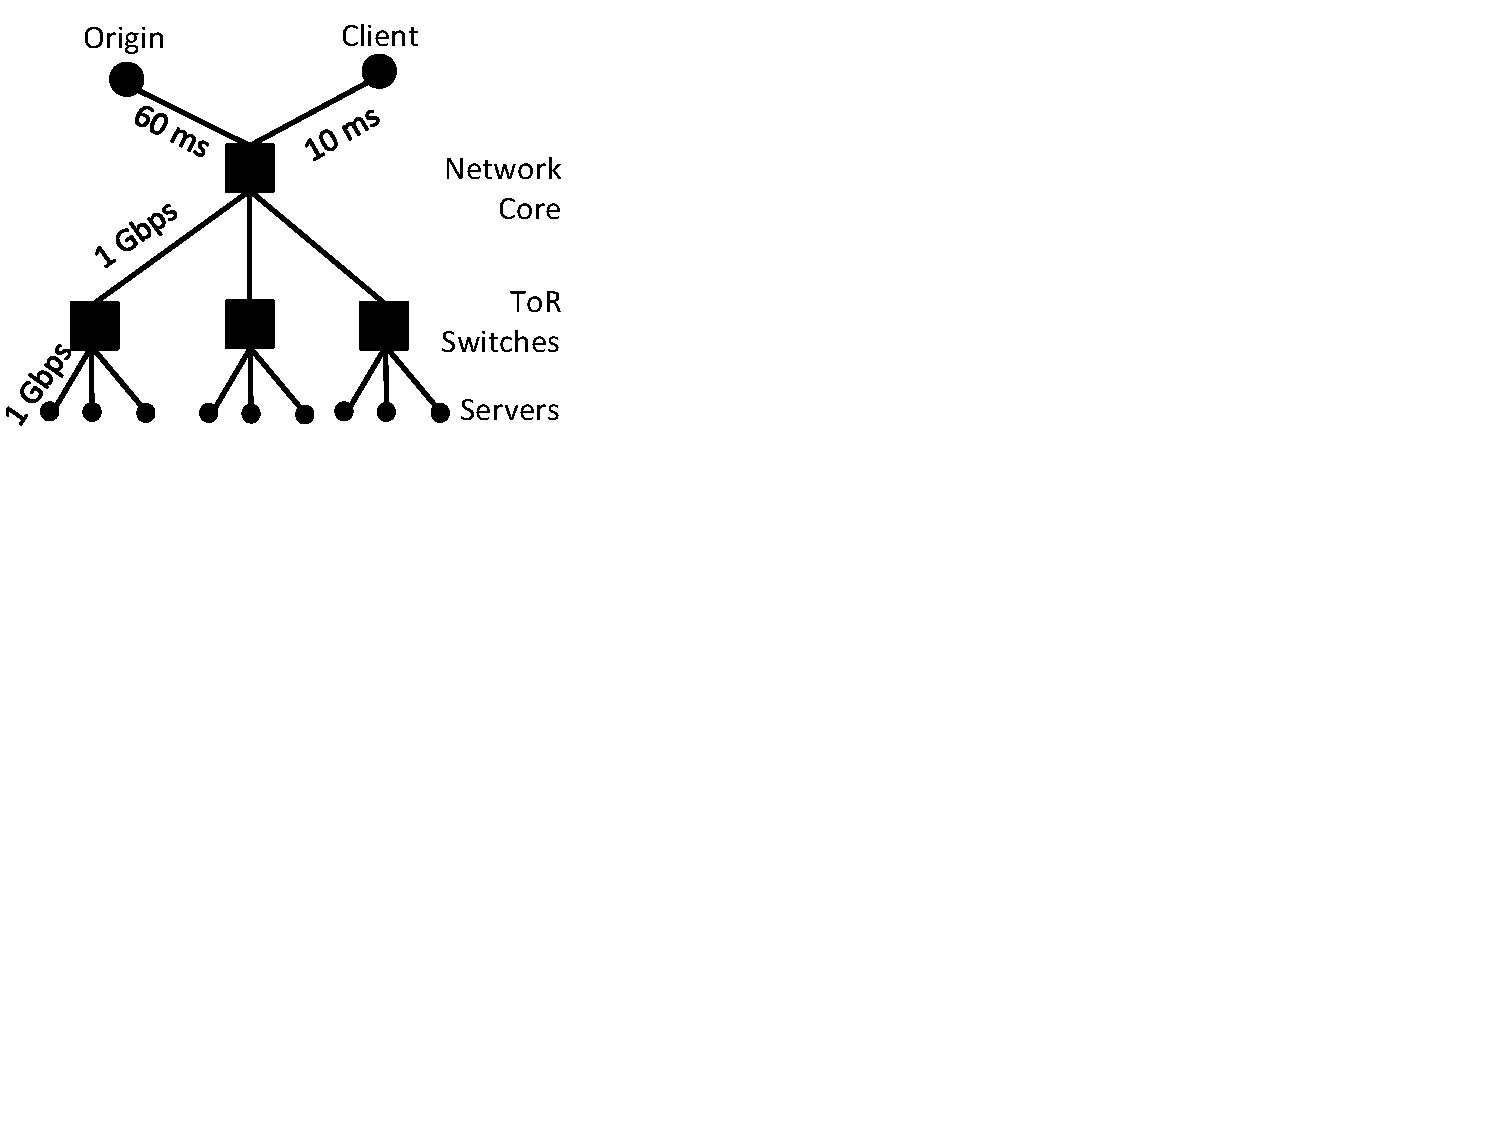
\includegraphics[scale=0.35]{figures/emulab-topo.pdf}
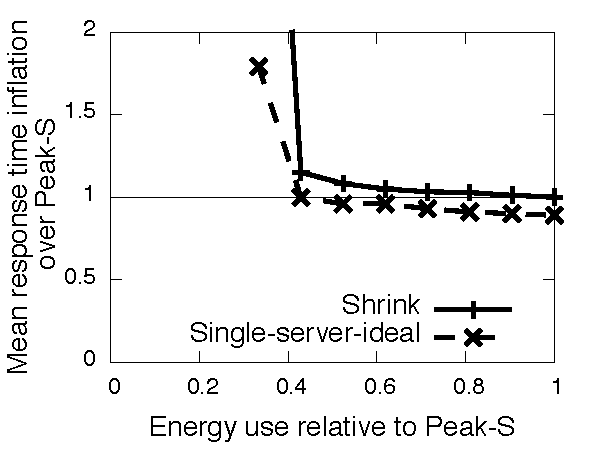
\includegraphics[scale=0.5]{graphs/final/emulab-mean.pdf}
\caption{Network and server consolidation (Section \ref{sec:emulab}): [Left] Emulab topology for the experiment. [Right] Compared to \peakS, \shrink\ has a 15\% higher response time but a 57\% lower energy use.}
\label{fig:emulab}
\end{figure}

We use Emulab to evaluate the energy-response time tradeoff when both server and network consolidation are being performed. For our experiment, we configure a tree topology with 1 Gbps links as shown in Figure \ref{fig:emulab} (left). 
In this topology, the ToR switches have 4 ports, and the core switch has at least 4 ports. Accordingly,  we calculate energy use of switches based on the power use of 4-port switch (Netgear GS105), which is 14.4 W \cite{netgearGS105}. The energy use of servers is computed using the same function as in the previous experiment. Our workload consists of a 1-hour duration of the trace containing requests for one-eighth of the content selected randomly.

Figure \ref{fig:emulab} (right) compares schemes in terms of the mean response times.  Across different runs that vary specified mean response times, \shrink\ uses between 2 and 9 servers; \peakS\ uses 9 servers.  We discuss the case when \shrink\ uses 3 servers so that only one of the ToR switches are being used as a result of network consolidation. In this case, the peak utilization of the link between the ToR and the core switch increased up to 76\% during the experiment, which is nearly three times higher than the peak link utilization for \peakS. Despite this increase, \shrink's response time is only 15\% higher than \peakS, while its network energy use is 50\% lower and the overall energy use is 57\% lower than \peakS\ (second point from the left in Figure \ref{fig:emulab} (right)). This result shows that both network and server consolidation can be performed with a small performance impact in \cdc s. Finally, we note that the difference between Single-server-ideal and \shrink\ is consistent with the difference between them in our experiment with server-only consolidation,, e.g., for the same energy savings as \shrink\ (= 57\%), \shrink's response time is 15\% more than Single-server-ideal.



%\begin{figure*}
%\begin{minipage}{0.3\textwidth}
%\centering
%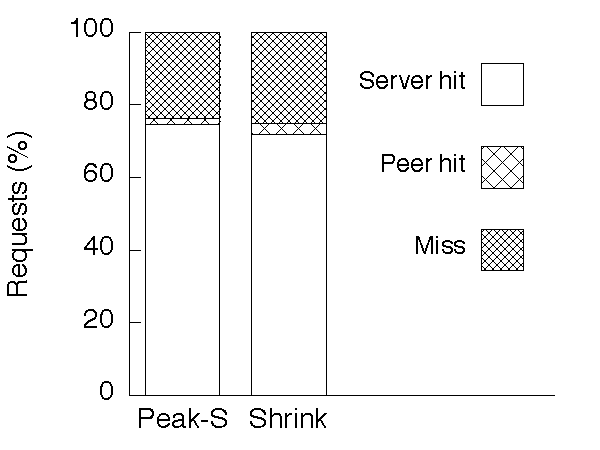
\includegraphics[scale=0.5]{graphs/final/sim-hitrate.pdf}
%\caption{[Simulator] \shrink\ increases miss rates by 1.5\% over \peakS\ over a one-week long trace showing that energy optimization in \cdc s hurts cache hit rates by a small margin. }
%\label{fig:sim-hitrate}
%\end{minipage}
%\hspace{0.5cm}
%\begin{minipage}{0.3\textwidth}
%\centering
%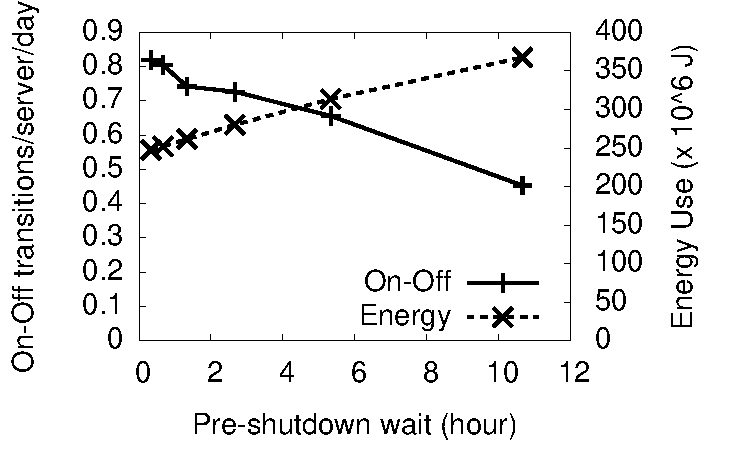
\includegraphics[scale=0.5]{graphs/final/onoff.pdf}
%\caption{[Simulator] Pre-shutdown wait interval ($W$) between 30 min \& 1 hour keeps on-off transition rate close to 1/server/day and with only a small increase in energy use over $W$ = 1 min.}
%\label{fig:sim-onoffrate}
%\end{minipage}
%\hspace{0.5cm}
%\begin{minipage}{0.3\textwidth}
%\centering
%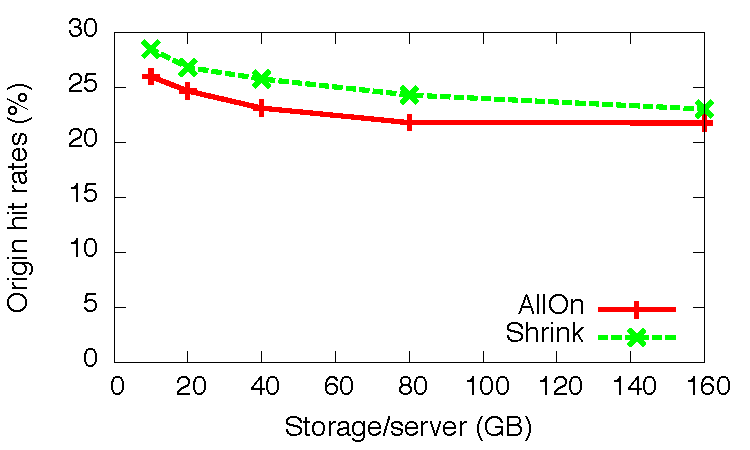
\includegraphics[scale=0.5]{graphs/final/storage.pdf}
%\caption{[Simulator] Difference between miss rates for both \shrink\ and \peakS\ is consistent despite variations in storage capacity.}
%\label{fig:sim-storage-vs-hitrate}
%\end{minipage}
%\end{figure*}

\subsubsection{Trace-based experiments}
\label{sec:simulation}
%The following are the goals of our trace-based experiments: (1) Quantify energy savings of server consolidation over the complete duration of the trace for a given server utilization limit expected to cause a small impact in response time.
%(2) Evaluate the potential benefit of cooperative caching among servers in a \cdc\ assuming that a cache-coordination protocol with a much smaller overhead can be developed in future. 
%(3) Quantify the tradeoff between energy savings and reliability by varying the pre-shutdown wait interval $W$.
%(4) Analyze the sensitivity of hit rates to a server's storage capacity.

\textbf{Methodology:} We conduct experiments for a \cdc\ with 16 servers for the week-long Akamai trace. The capacity of each server is defined in terms of network traffic it can support. The rate of network traffic generated by a request is a constant equal to the client bandwidth reported in the Akamai trace. To be able to fit the simulator process in the memory on our machine (32 GB), we filtered requests for one-eighth of the content from the trace. Accordingly, we scale down  the capacity of each server to be 150 Mbps, and the cache size per server to be 150 GB. Since trace-based experiments do not provide an accurate estimate of response times, we used a fixed server utilization limit $U$ = 0.65 for our experiments, which is expected to cause a small response time inflation (Figure \ref{fig:ec2-other} (right)). 
The cache hit rates of our simulator's LRU caching and Squid differ by less than 2\% for the same workload and cache size. 


\begin{figure}
\centering
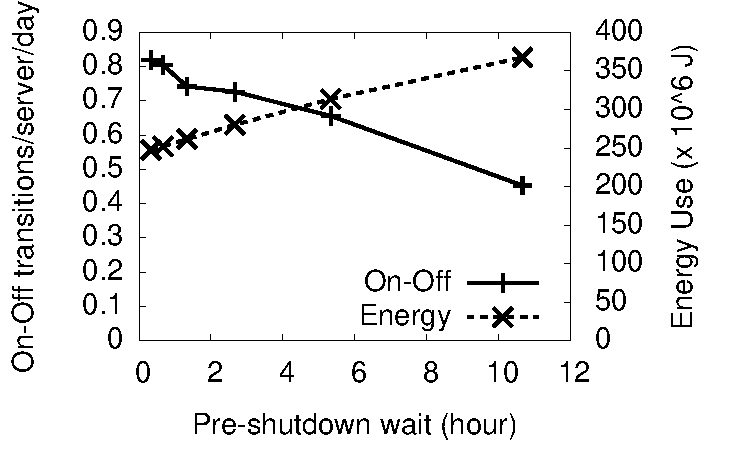
\includegraphics[scale=0.4]{graphs/final/onoff.pdf}
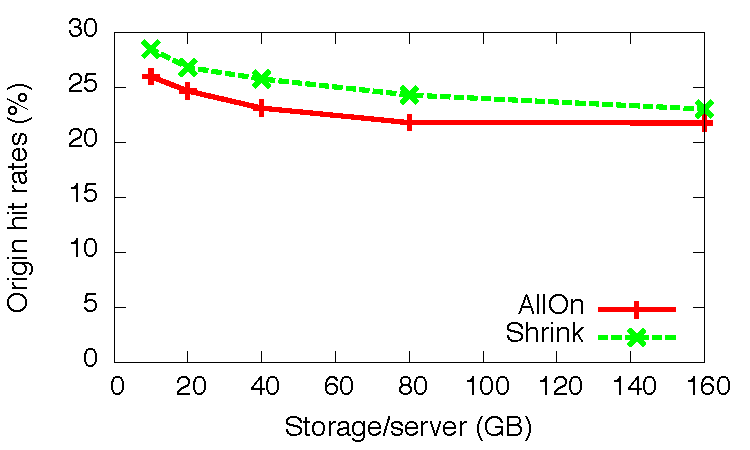
\includegraphics[scale=0.4]{graphs/final/storage.pdf}
\caption{[Simulator] [Left] Pre-shutdown wait interval between 30 min \& 1 hour keeps on-off transition rate close to 1/server/day. [Right] Comparison of miss rates for varying amounts of storage.}
\label{fig:sim-onoffrate}
\end{figure}
\textbf{Impact on hardware reliability:} Figure \ref{fig:sim-onoffrate} (left) shows the rate of on-off transitions per server and the corresponding energy savings is achievable. We find that a short pre-shutdown wait interval $W$ = 1 min hurts hardware reliability by increasing the rate of server transitions to more than 20/server/day. On the other hand, a  high $W$ = 4 hours reduces server transition rate to 0.81/server/day, but increases energy use by nearly 45\% over $W$ = 1 min.  The sweet spot for pre-shutdown wait interval is between 30 min to 1 hour, where increase in energy use over $W$ = 1 min is between 12\% and 15\%  but most of the reduction in on-off transition rates can still be achieved.

\textbf{Storage vs. cache miss rates:} To determine the sensitivity of miss rates to available storage, we evaluate \peakS\  and \shrink\ for varying amount of storage from 10 GB/server to 160 GB/server and present results in Figure \ref{fig:sim-onoffrate} (right). We remark that we have scaled down the CDN trace and hence the storage by a 8$\times$ factor, i.e., we would have provisioned 1.28 TB storage instead of 160 GB if we were to experiment with the full trace.  As storage reduces, the miss rates increase as expected. But, the relative difference between miss rates for both \shrink\ and \peakS\  remains nearly the same even on reducing the storage to 10 GB, e.g., \shrink's miss rates are 10.3\% higher than that of \peakS\  for 160 GB storage and are 9.6\% higher than that of \peakS\  for 10 GB storage. Thus, we conclude that server consolidation schemes are expected to increase datacenter miss rates by a small fraction within the range of storage typically available on server-class machines. 

\textbf{Cooperative caching benefit:} We evaluate the potential benefit of cooperative caching among servers in a \cdc\ assuming that a cache-coordination protocol with a much smaller overhead can be developed in future. The hit rates at cache peers  are 1.65\% for \peakS\  and 3.02\% for \shrink, which suggests that cooperative caching among datacenter servers, if implemented efficiently, could reduce the impact of energy optimization schemes by a small margin. 
%We present other results from trace-based experiments here. 
%(1) Over a one-week long trace. \shrink\ provides 37\% energy savings over \peakS. (2) 

%\textbf{Energy savings and cache hit rates:}
%We have compared the energy use of \shrink\ against other schemes over a one-week long trace. \shrink\ provides 37\% energy savings over \peakS\ in that experiment. We skip a detailed discussion of the results noting that energy use of other schemes are qualitatively similar to that observed in the experiment on EC2.
%
%Figure \ref{fig:sim-hitrate} compares the server hit rates, peer hit rates and miss rates. We make two key observations from this graph. First, there is less than 1.5\% difference in miss rates between \shrink\ and \peakS\  scheme, which supports our earlier observation in prototype-based experiments that \shrink's energy optimization does cause a significant increase in miss rates.  Second, we note that peer hit rates are 1.65\% for \peakS\  and 3.02\% for \shrink, which suggests that cooperative caching among datacenter servers could reduce the impact of energy optimization schemes by a small margin. Implementing a cooperative caching scheme with a low overhead is a topic of future work.




\eat{
%\begin{figure}
%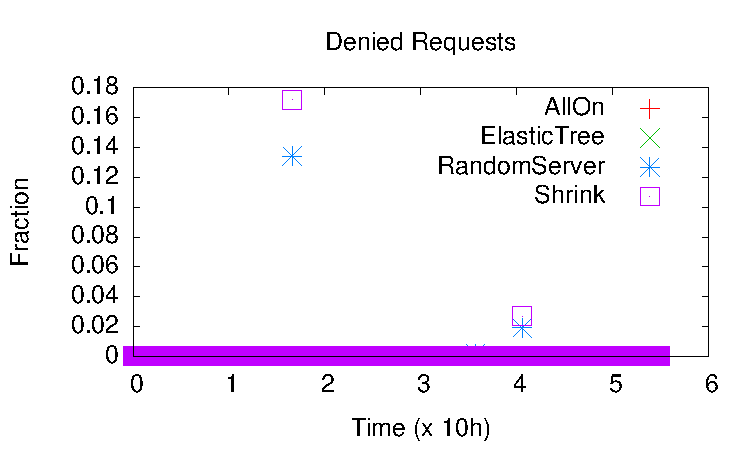
\includegraphics[scale=0.6]{graphs/server-logs/denied.pdf}
%\caption{Fraction of requests that are denied. \peakS\  scheme denies no requests throughout the experiment, whereas other schemes have a non-zero denied requests in a few time intervals. Both intervals  where requests are denied happened in cases of sudden spikes in load during night time.}
%\label{fig:sim-availability}
%\end{figure}

Figure \ref{fig:sim-availability} shows the fraction of requests that are denied due to server unavailability. Each data point represents denied requests in a 5-min interval. We find that the \peakS\  scheme has no denied requests throughout the experiment, i.e., it has 100\% availability. \shrink\ also has 100\% in all time intervals, except for two. Further analysis showed that both these intervals occured in late-night hours between 2 AM and 4 AM when there was unexpected spike in load that was 4 times the expected load in that interval. The active servers at that time did not sufficient enough resources to handle the request load. Thus, there was a brief period of unavailability until more servers could be turned on. That server unavailability is near-perfect an encouraging sign for deploying server consolidation, but also shows that energy-optimizing schemes make a \cdc\ less tolerant to highly unpredictable increase in load. A possible way to reduce the impact of such unavailability is to keep servers in a sleep state instead of completely turning them off so that they can be turned on quickly if necessary. 
}

%\begin{figure}
%\centering
%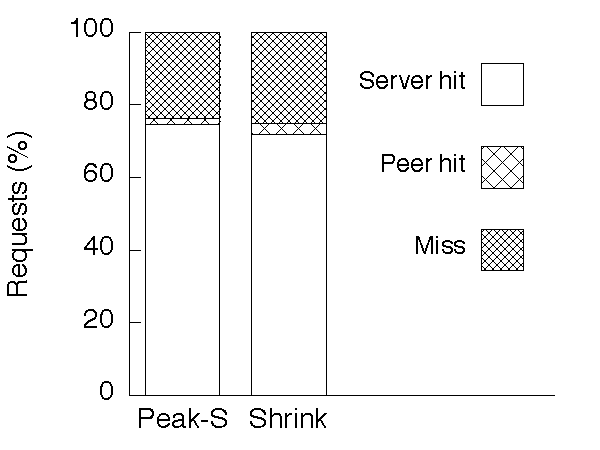
\includegraphics[scale=0.6]{graphs/final/sim-hitrate.pdf}
%\caption{[Simulator] \shrink\ increases miss rates by a small margin of 1.5\% over \peakS\ over a one-week long trace showing that energy optimization in \cdc s hurts cache performance by a small margin. }
%\label{fig:sim-hitrate}
%\end{figure}



%\begin{figure}
%\centering
%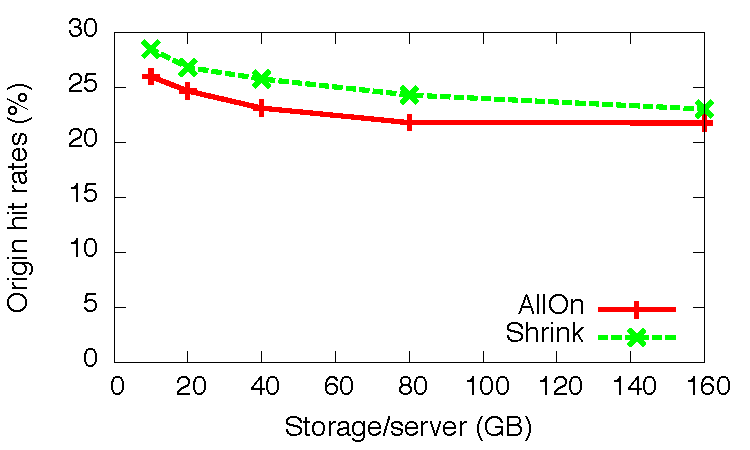
\includegraphics[scale=0.6]{graphs/final/storage.pdf}
%\caption{}
%\label{fig:sim-storage-vs-hitrate}
%\end{figure}




%%!TEX root = Main.tex




\subsection{End-to-end mobility case studies}
\label{sec:e2e}

\begin{figure*}[ht]
	\vspace{0.05in}
	\begin{minipage}[b]{0.48\linewidth}
		\centering
		\includegraphics[width=2.8in,height=1.4in]{graph/newgraphs/managed-lookup.pdf}
		\figvsp
		\caption{Lookup latency:  \auspice\ with 5 replicas is comparable to UltraDNS (16 replicas); \auspice\ with 15 replicas has 60\% lower latency than UltraDNS.}
		\label{fig:managed-lookup}
	\end{minipage}
	\hspace{0.2in}
	\begin{minipage}[b]{0.48\linewidth}
		\centering
		\includegraphics[width=2.8in,height=1.4in]{graph/newgraphs/managed-update.pdf}
		\figvsp
		\caption{Update propagation delay: \auspice\ with 5 replicas is  1.0 to 24.7 secs lower than three top-tier managed DNS service providers. }
		\label{fig:manageddnsupdate}
	\end{minipage}
	%\hspace{0.3cm}
	%\begin{minipage}[b]{0.3\linewidth}
	%\centering
	%\includegraphics[width=2in,height=1.5in]{graph/medianlatencyVSlocality.pdf}
	%\figvsp
	%\caption{[Simulator] Workload sensitivity: \auspice\ lowers latency by 2--5$\times$  over \staticthree\ at all geo-locality levels.}
	%\label{fig:varylocality}
	%\end{minipage}
	\vspace{-0.25in}
\end{figure*}



Can \auspice\ serve as the basis of a complete end-to-end mobility solution? To address this question, we have developed \msocket, a user-level socket library that interoperates with \auspice, and supports all four types of endpoint mobility. %Using \auspice, \msocket\  supports connection migration, multipath communication, and mobile-to-mobile communication despite address-translating middleboxes using a distributed proxy service. 
The details of \msocket's design and implementation is the subject of a separate paper \cite{msocketTR}. Here, we {\em use} \msocket\ to show proof-of-concept of some of \auspice's capabilities.

\subsubsection{Time-to-connect to ``moving'' endpoints}
\label{sec:ttc_exp}

We evaluate the time-to-connect to a moving destination as a function of the mobility (or update) rate. The {\em end-to-end time-to-connect}  here is measured as the latency to look up an up-to-date address of the destination (or the time-to-connect as defined in $\S$\ref{sec:design_overview}) plus the time for msocket to successfully establish a TCP connection between the client and the mobile destination. This e2e-time-to-connect also incorporates the impact of timeouts and retried lookups if the client happens to have obtained a stale value (as in Fig. \ref{fig:4mobility}). The experiment is conducted on PlanetLab and consists of a single msocket client and a single mobile msocket server that is ``moving'' by changing its listening port number on a remote machine, and updating the name record replicated on three \auspice\ name servers accordingly. 
A successful connection setup delay using msocket is takes 2 RTTs (2 $\times$ 105 ms)  \cite{msocketTR}. 
As defined in Eq. \ref{eq:ttc}, the values of the update propagation latency $d_i$ and the lookup latency $l_i$ are 250 ms and 20 ms respectively, and the update rate $w_i$ varies from 1/1024/s to 1/s.
The timeout value ($T$) in our experiment is dependent on the RTT between the client and the server. If the client attempts to connect to the server on a port which the server is not listening on, the server immediately returns an error response to the client. Specifically, the timeout value is either 1 or 2 RTTs with equal probability depending on whether the connection failed during the first or the second round-trip of msocket's connection setup.
The client sends lookups at a rate of 10/s (but this rate does not affect the time-to-connect), and both lookups and updates inter-arrival times are exponentially distributed.


Figure \ref{fig:ttc_msocket} shows the distribution of the time-to-connect with update propagation delays entailed by eventual consistency. For low-to-moderate mobility rates ($<\frac{1}{64s}$), we find that all time-to-connect values are close to 230 ms, of which 20ms is the lookup latency, and 210ms is msocket's connection setup latency. The reason the client is able to obtain the correct value upon first lookup in all cases is that the update propagation latency of 250ms is much smaller than the average inter-update interval (64s).  The update propagation delay becomes a non-trivial fraction of the inter-update interval at high mobility rates of $\approx$1/sec that results in  26\% of lookups returning stale values. The mean e2e-time-to-connect increases to  302 ms for an update rate of 1/sec, which suggests that \auspice's time-to-connect is limited by network propagation delays in this regime. Nevertheless, once a connection is successfully established, {individual} migration can quickly resynchronize the connection in $\approx$two round-trips between the client and the mobile without relying on \auspice\ (not shown here). 
%A different experiment with totally ordered writes shows qualitatively similar conclusions \cite{techreport}.

Figure \ref{fig:ttc_msocket} also shows that the time-to-connect as predicted by our analytical model (Eq. \ref{eq:ttc}) are close to those observed in the experiment, thereby re-affirming our design. 

%\blue{We evaluate the time-to-connect to a moving destination as a function of the mobility (or update) rate. We stick with the running definition of time-to-connect used in the paper, namely, the time to look up an up-to-date address of the destination, i.e., an address to which the client can successfully establish a TCP connection. This definition excludes the (successful) connection setup delay itself as that delay is independent of \auspice's design, but it does incorporate the impact of timeouts and retried lookups if the client happens to have obtained a stale value (as in Fig. \ref{fig:4mobility}). The experiment is conducted on PlanetLab and consists of a single virtual client and a single virtual mobile server that is ``moving'' by changing its listening port number on a remote machine, and updating the name record replicated on three \auspice\ name servers accordingly. As defined in Eq. \ref{eq:ttc}, the values of the timeout $T_i$ and lookup latency $l_i$ are 5 secs and 50 ms respectively, and the update rate $w_i$ varies from $10^{-4}$/s to 1/s. The client sends lookups at a rate of 10/s (but this rate does not affect the time-to-connect), and both lookup and update inter-arrival times are exponentially distributed}

%\blue{Figure \ref{fig:ttc} shows the distribution of the time-to-connect with update propagation delays entailed by eventual consistency. For low-to-moderate mobility rates ($< 0.01/$s), we find that all lookup latencies are much smaller than 5 sec and mean time-to-connect is less than 50 ms, i.e.,  the client is able to obtain the correct value upon first lookup in all cases. This is because the update propagation latency of 190 ms is much smaller than the average inter-update interval (100 s).  The update propagation delay becomes a non-trivial fraction of the inter-update interval at high mobility rates of 0.1 to 1/sec that respectively result in 1.5\% and 13\% of timeouts for lookups. The mean time-to-connect increases to  641 ms for an update rate of 1/sec, which suggests that \auspice's time-to-connect is limited by network propagation delays in this regime. Nevertheless, once a connection is successfully established, {individual} migration can quickly resynchronize the connection in about two round-trips between the client and the mobile without relying on \auspice\ (not shown here). %A different experiment with totally ordered writes shows qualitatively similar conclusions \cite{techreport}.}

%\blue{Figure \ref{fig:ttc} also shows that the time-to-connect as predicted by our analytical model (Eq. \ref{eq:ttc}) is close to those observed in the experiment, thereby re-affirming our design. }

\eat {
	% sequential single-column figures
	
	\begin{figure}[ht]
		\vsp
		\centering
		\includegraphics[width=3in, height=1.5in]{figure/SimulMig.pdf}
		\figvsp
		\caption{Simultaneous mobility recovery in $\approx$2 RTTs after both endpoints resurface.}
		\label{fig:SimulMig}
	\end{figure}
	
	\begin{figure}[ht]
		\figvsp
		\centering
		\includegraphics[width=2in, height=1.5in]{figure/5MemTimeLineUsed.pdf}
		\figvsp
		\caption{Context-aware delivery timeline showing 3 messages being geo-cast to 5 members.}
		\label{fig:5MemberTimeline}
		\figvsp
	\end{figure}
}





\subsubsection{Simultaneous endpoint mobility}

Figure \ref{fig:SimulMig} shows an experiment involving simultaneous mobility. The client is an Android phone using \msocket\ via a WiFi interface to connect to a publicly addressable Planetlab machine at time 0. The server and client shut down their interfaces respectively around 15 and 20 sec. Subsequently, the server restarts its interface and starts listening on a different port and updates \auspice\ accordingly. After that, the client restarts its interface and attempts to re-synchronize the connection. This re-synchronization time is roughly 300ms as shown and consists of the following delays. The client performs a query to \auspice\ to resolve the server's GUID to its new socket address (IP, port), which takes roughly 50ms and mostly corresponds to the round-trip delay between the client and the \auspice\ nameserver. The remaining 250ms roughly correspond to 2 RTTs of delay between the client and the server that are separated by a round-trip delay of 120ms.

\subsubsection{Context-aware delivery}
\label{sec:context}

Next, we show a proof of concept of context-aware communication, a novel communication primitive enabled by \auspice's extensible key-value API. \auspice\ allows applications to bind an \msocket\ not only to human-readable names or GUIDs, but also to abstract context descriptors as in \verb+msocket.bind("[geoloc: [lat,long],radius]")+.  Writes to this \msocket\ are reliably delivered to all GUIDs in the geo-fence created by this descriptor. Underneath the covers, \msocket\ invokes \auspice\ to create on-demand a {group GUID}, i.e., a  GUID with a membership field consisting of a set of member GUIDs, and obtains this member set. \msocket\ internally resolves each member GUID to its socket address and establishes an \msocket\ connection for reliably delivery.

Figure \ref{fig:5MemberTimeline} shows an experiment involving a group creator (also the message sender) on an Android phone and a number of potential members on PlanetLab nodes, 5 of which fake-register their coordinates in \auspice\ so as to appear to be within the created geo-fence. The RTT between the group creator and members is 125ms. The figure shows that group creation, a single call to \auspice\ that returns all member GUIDs, takes roughly 200ms. Subsequently, an internal \msocket\ connect to each member involves another \auspice\ lookup to resolve the GUID to a socket address and connect in parallel to all 5 members, which takes 250-280ms. After this, the creator sends 3 short messages back-to-back that each take roughly 1 RTT to be reliably delivered.

%Context-aware group GUIDs in \auspice\ are active, i.e., \auspice\ refreshes the membership set periodically so that if an existing member leaves or a new member arrives into the context-space, the group GUID is updated accordingly. This refresh interval limits how responsive context-aware communication is to member churn. 
More details of optimizing context-aware queries in \auspice, reducing membership staleness, the connection migration protocol, etc. are outside the scope of this paper \cite{msocketTR}. This experiment seeks only to exemplify a powerful, new communication primitive enabled by context descriptors compared to strictly hierarchical DNS names, as argued in $\S$\ref{sec:whyNotDNS}. 

















\begin{figure*}[ht]
\vspace{0.05in}
\begin{minipage}[b]{0.48\linewidth}
\centering
\includegraphics[scale=0.55]{graph/newgraphs/managed-lookup.pdf}
\figvsp
\caption{Lookup latency:  \auspice\ with 5 replicas is comparable to UltraDNS (16 replicas); \auspice\ with 15 replicas has 60\% lower latency than UltraDNS.}
\label{fig:managed-lookup}
\end{minipage}
\hspace{0.2in}
\begin{minipage}[b]{0.48\linewidth}
\centering
\includegraphics[scale=0.55]{graph/newgraphs/managed-update.pdf}
\figvsp
\caption{Update propagation delay: \auspice\ with 5 replicas is  1.0 to 24.7 secs lower than three top-tier managed DNS service providers. }
\label{fig:manageddnsupdate}
\end{minipage}
%\hspace{0.3cm}
%\begin{minipage}[b]{0.3\linewidth}
%\centering
%\includegraphics[width=2in,height=1.5in]{graph/medianlatencyVSlocality.pdf}
%\figvsp
%\caption{[Simulator] Workload sensitivity: \auspice\ lowers latency by 2--5$\times$  over \staticthree\ at all geo-locality levels.}
%\label{fig:varylocality}
%\end{minipage}
\vspace{-0.25in}
\end{figure*}
 
 
\vsp
\subsection{\auspice\ vs. managed DNS providers}
\label{sec:managed}
%In DNS terminology, an \auspice\ name server provides the functionality of an authoritative name server -- it keeps the most up to date  name-to-address mapping of a host.
 

Can demand-aware replication benefit commercial managed DNS providers that largely rely on statically replicating today's (hardly mobile) domain names? To investigate this, we compare \auspice\ against three top-tier providers, UltraDNS, DynDNS, and DNSMadeEasy %\cite{ultradns, dyndns, dnsmadeeasy}, 
that offer geo-replicated authoritative DNS services widely used by enterprises (e.g., Dyn provides DNS service for Twitter).


%Having analyzed a synthetic workload dominated by mobile device names, we next evaluate how \auspice\ compares to commercial managed DNS providers in serving their customers' (mostly static) domain names.  These providers such as UltraDNS, DynDNS, and DNSMadeEasy \cite{ultradns, dyndns, dnsmadeeasy} offer a geo-replicated authoritative DNS service and are widely used by enterprises today (e.g., DynDNS provides DNS service for Twitter).

%Similar to the role of a replica of a name record in \auspice, managed DNS providers such as UltraDNS, DynDNS, and DNSMadeEasy \cite{ultradns, dyndns, dnsmadeeasy}  offer a geo-replicated authoritative DNS service for domain names.%\footnote{DNS Services such as Open DNS \cite{opendns}, and Google DNS \cite{googledns} maintain local name servers that store cached name records  and therefore are not managed DNS services.}

%Note that Open DNS \cite{opendns}, Google DNS \cite{googledns} and other similar services which offer name lookup service to their users  maintain local name servers that store cached name records  and therefore are not managed DNS services. 


%Managed DNS providers such as UltraDNS, DynDNS, and DNSMadeEasy \cite{ultradns, dyndns, dnsmadeeasy} offer a geo-replicated authoritative DNS service similar to \auspice.
%Managed DNS providers differ from services such as Open DNS \cite{opendns}  and Google DNS \cite{googledns} as the former maintain authoritative name servers for domain names of their customers and the latter maintain local name servers that store cached name records. 



%Managed DNS providers \cite{ultradns,dyndns,dnsmadeeasy} offer a geo-replicated DNS service, and are commonly purchased by enterprises today. This section compares \auspice\ to managed DNS providers in terms of lookup and update latencies. 

\subsubsection{Lookup latency}  


We compare \auspice\ to UltraDNS for a workload of lookups for  domain names serviced by the provider. We identify 316 domain names among the top 10K Alexa websites serviced by this provider, and determine
the geo-distribution of lookups for each name from their data \cite{alexa}.
For each name, we measure the latency for 1000 lookups from across 100 PlanetLab nodes. 
We ensure that lookups are served from the name servers maintained by the provider by requesting the address for a new random sub-domain name each time, e.g, \verb+xqf4p.google.com+ instead of \verb+google.com+, that is unlikely to exist in a cache and requires an authoritative lookup.
\auspice\ name servers are deployed across a total of 80 PlanetLab locations while UltraDNS has 16 known server locations \cite{dnscompare}.  
We evaluate \auspice\ for three configurations  with 5, 10, and 15 replicas of a name respectively. 

%For an even comparison between \auspice\ and the provider, we limit the maximum number of replicas/name for \auspice\ to 5, which is less than one-third the number of locations of the provider \cite{dnscompare}.  
%The geo-distribution of lookups for each domain name is determined based on the Alexa dataset \cite{alexa}.




%The list of MDNS deployments is obtained from this report \cite{dnscompare}. The median and maximum different between \auspice\ name server and the corresponding MDNS deployment was X miles and Y miles respectively.  



%\begin{figure}[t]
%\centering
%\includegraphics[scale=0.6]{graph/camera-ready/managed-lookup.pdf}
%\vspace{-0.2in}
%\caption{\auspice\ gives better cost-performance tradeoffs than UltraDNS. \auspice\ with 5 replicas has comparable latency to UltraDNS (16 replicas); \auspice\ with 15 replicas has 60\% lower lookup latencies than UltraDNS. Box plot shows 5, 25, 50, 75, and 95 percentiles.}
%\label{fig:managed-lookup}
%\end{figure}

\blue{
Figure \ref{fig:managed-lookup} shows the lookup latencies of names for \auspice\ and for UltraDNS.
UltraDNS incurs a median latency of 45 ms with 16 replicas,  while \auspice\ incurs  41 ms, 22 ms, and 18 ms  respectively with 5, 10, and 15 replicas. 
With 5 replicas, \auspice's performance is comparable to UltraDNS with one-third  the replication cost. 
With 15 replicas, \auspice\ incurs 60\% lower latency for a comparable cost. The comparison against the other two, Dyn and DNSMadeEasy, is qualitatively similar \cite{techreport}.
Thus, \auspice's demand-aware replication achieves a better cost--performance tradeoff compared to static replication.
}




\subsubsection{Update propagation delay} 
To measure update propagation delays, we purchase DNS service from three providers for separate domain names.  All providers replicate a name at 5 locations across US and Europe for the services we purchased. We issue address updates for the domain name serviced by that provider and then immediately start lookups to the authoritative name servers for our domain name.
These authoritative name servers can be queried only via an anycast IP address, i.e., servers at different locations advertise the same externally visible IP address. Therefore, to maximize the number of provider locations queried, we send queries from 50 random PlanetLab nodes. From each location, we periodically send queries until all authoritative name server replicas return the updated address.  The update propagation latency at a node is the time between when the node starts sending lookup to when it receives the updated address. The latency of an update is the the maximum update latency measured at any of the nodes. We measure latency of 100 updates for each provider.
 %is time difference between when we update an address and when the node gets the updated address. 

To measure update latencies for \auspice, we replicate 1000 names at a fixed number of PlanetLab nodes across US and Europe. The number of nodes is chosen to be 5, 10, and 20 across three experiments. A client sends an update to the nearest node and waits for update confirmation messages from all replicas. The latency of an update is the time difference between when the client sent an update and when it received the update confirmation message from all replicas (an upper bound on the update propagation delay).  We show the distribution of measured update latencies for \auspice\ and for three managed DNS providers in Figure \ref{fig:manageddnsupdate}.   

\auspice\ incurs lower update propagation latencies than all three providers for an equal or greater number of replica locations for names. We were unable to ascertain from UltraDNS why their update latencies are an order of magnitude higher than network propagation delays, but this finding is consistent with a recent study \cite{dnscompare} that has shown latencies of up to tens of seconds for these providers. Indeed, some providers even distinguish themselves by advertising shorter update propagation delays than competitors \cite{dnscompare}.


\subsection{Sensitivity analyses and other results.} 
\label{sec:other} 
We have conducted a comprehensive evaluation of the sensitivity of \auspice's performance-cost trade-offs to workload and system parameters across scales varying by several orders of magnitude. These include workload parameters such as geo-locality, read-to-write rate ratio, ratio of device-to-service names, etc. and system parameters such as the fault-tolerance threshold, capacity utilization, perturbation knob, the tunable overhead of replica reconfiguration, etc. using a combination of simulation and system experiments. These results do not qualitatively change the above findings, and are deferred to the technical report \cite{techreport}.

%To assess the sensitivity of \auspice's benefits to a broad range of system and workload parameters and scales, we develop a custom simulator that simulates round-trip delays, loss, and server load-vs-response time behavior, and have verified \cite{techreport} that the median latencies for all simulated schemes are within 8\% of those in $\S$\ref{sec:comparison}. We present one such experiment here, deferring others to a technical report \cite{techreport}.

%Figure \ref{fig:varylocality} compares the latency for workloads with varying  geo-locality. Both \staticthree\ and \codons\ are choose replica locations randomly, and therefore their latency remains the same irrespective of the workload's geo-locality. But \auspice\ significantly improves latencies  as the geo-locality increases. Even in a workload with no locality ($g$=0.1),   \auspice\ outperforms \staticthree\ by 2$\times$ because it creates more than three replicas for each name,  and outperforms \codons\ by $4\times$  because it redirects requests to the closest replica of a name without DHT routing.

%Other experiments evaluating the sensitivity of \auspice's performance-cost trade-offs at different scales to workload parameters such as the ratio of device-to-service names, overall lookup-to-update ratio, and system parameters such as the fault-tolerance, capacity utilization, and reconfiguration epoch length are deferred to the technical report \cite{techreport}.

\rmCR{
\subsection{Simulation-based sensitivity analysis}
\label{sec:sensitivity}

In order to assess the sensitivity of \auspice's performance and cost to a wider range of system parameters, workload parameters in $\S$\ref{sec:comparison}, and scales, we use a custom simulator that simulates round-trip delays, loss, and server load-vs-response time behavior as in the PlanetLab experimental setup. We have verified \cite{techreport} that the median latencies for all simulated schemes are within 8\% of those in the emulation in $\S$\ref{sec:comparison}.   Experiments here use 10K name servers, 2K local name servers, 10K service names, and 100K device names. 

%We analyze the sensitivity of \auspice's benefits to the workload parameters used in $\S$\ref{sec:comparison}. In order to be able to explore a wider range of parameters and scales, we use a custom simulator that simulates round-trip latency, loss, and server load-vs-response time behavior as measured on PlanetLab. We have verified \cite{techreport} that the median latencies for all schemes in the simulator are within 8\% of that on PlanetLab for the experiment in $\S$\ref{sec:comparison}.   Experiments here use 10K nameservers, 2K local nameservers, 10K service names, and 100K device names. 

\textbf{Geo-locality.}  Figure \ref{fig:varylocality} compares the latency for workloads with varying levels of geo-locality.
Both \staticthree\ and \codons\ are choose replica locations randomly, and therefore their latency remains the same irrespective of the workload's geo-locality. But \auspice\ significantly improves latencies  as the geo-locality increases. Even in a workload with no locality ($g$=0.1),   \auspice\ outperforms \staticthree\ by 2$\times$ because it creates more than three replicas for each name,  and outperforms \codons\ by $4\times$  because it redirects requests to the closest replica of a name without the overhead of DHT routing.

\textbf{Ratio of device-to-service names.} We also evaluate schemes for workloads with different ratios of device names to service names. We fix the number of service names to be 10K and vary the number of device names between 1000 to 1M.
%\replicateall\  saturates server capacity for a workload with  DS-ratio = 1 due to high update costs. 
For the given capacity, \auspice\  can accommodate a workload with up 1M device names (while \replicateall\ can support at most 1K device names) and provides up to 6.9$\times$ lower latencies over \staticthree\  across for all ratios of service-to-device names.

% up to 100  as it minimizes the update cost for device names. 
% \auspice\ has up to 6.9$\times$ lower latency than \staticthree\ and \codons\ due to itts locality-aware design,

\textbf{Lookup-to-update ratio.} We vary the ratio of lookups to updates, termed as \emph{RW-ratio}, by increasing the number of lookups but keeping the number of updates fixed. \auspice\ provides up to 2.95$\times$ lower latencies than \codons\ and \staticthree\ for both write-dominated workload (RW-ratio $<$ 1) as well as read-dominated workloads (RW-ratio  $>$ 1). As RW-ratios increase beyond 1,  \auspice\ handles the increase in number of lookups  by automatically decreasing the replication parameter $\beta$ (refer to Eq. \ref{eq:mu}).

\blue{
\textbf{System parameters.} We also experiment with the system parameters in $\S$\ref{sec:design}, the fault tolerance threshold $F$, the capacity utilization $\mu$, and the randomness knob $\nu$. As expected, we find that as $F$ increases and approaches the total number of name servers, the cost and performance behavior increasingly mimics \static{F} until it is identical to \replicateall. Decreasing $\mu$ to small values makes \auspice's replication less aggressive hurting performance but reducing cost, while increasing $\mu$ much closer to 1 hurts latencies by overloading the system. The technical report \cite{techreport} describes these results as well as a slightly modified replica placement strategy that makes the random perturbation knob $\nu$ unnecessary (currently manually set to 0.5 in our experiments).
}
}


%\textbf{Lookup rate distribution:} We evaluate performance for (a) Zipf  and (b) uniform popularity distribution of  lookup rates of users The mean lookup rates are same for both distributions. As Figure \ref{fig:lookupdis} shows, the lookup latency of all schemes are nearly equal for the two distributions.  The performance of \staticthree\ is unchanged because its replica placement is fixed. \codons\ sees high latency for both distributions because its design replicates most names at a small number of locations for both distributions (a small percent of highly popular names are replicated at larger number of locations). The median lookup rates are smaller for Zipf-distribution compared to uniform distribution, i.e., a typical name has a smaller read-to-write ratio for Zipf-distritbution compared to uniform distribution . Hence, \auspice\ create less number of replicas for most names. Still, the number of replicas for names is sufficiently high in this experiment to keep the lookup latency nearly the same. 

%The slightly better latencies for \auspice\ for the Zipf-distribtuion are because of  highly popularity names see a improv

%\codons\ decides number of replicas only based on popularity ranking of a name and not on the value of the lookup rates, and hence its distribution of the number of replicas of names remains unchanged due to a change in the popularity distribution. 

%The performance of \codons\ and \staticthree\ are unchanged as they 

%Across experiments, we change the distribution of lookup rates of users keeping the average lookup rate unchanged.  Figure X shows the results. 

%This experiment suggests that our results from prior experiments are likely to hold irrespective of the specific distribution of lookup rates of users.


\eat{
\begin{figure}
\centering
\includegraphics[scale=0.5]{graph/medianlatencyVSnummobile.pdf}
\vspace{-0.1in}
\caption{[Simulator] \auspice\ gives greater latency gains over \staticthree\ as the number of device names increases in  the workload.}
\label{fig:varymobile}
\end{figure}

\textbf{Ratio of device names to service names:} This experiment evaluates schemes for workloads with different ratios of device names to service names, called \emph{DS-ratio} for short.
We fix the number of service names to be 10K and vary the number of device names between 1000 to 1,000,000.
Figure \ref{fig:varymobile} presents our results.
\replicateall\  saturates server capacity for a workload with  DS-ratio = 1 due to high update costs. 
\auspice\  supports workloads with DS-ratio up to 100  as it minimizes the update cost for device names. 
Due to its locality-aware design, \auspice\ has  2.6$\times$, 4.5$\times$ and 6.9$\times$ lower latency than \staticthree\ when DS-ratios are 1, 10 and 100 respectively. 

\textcolor{blue}{
 \codons's latency increases more sharply than \auspice\ and \staticthree\  on increasing the number of device names.  
\codons\ creates  a greater number of replicas for device names than \auspice\ and \staticthree, which increases update cost and, as a result, the lookup latency for \codons.
For example, for a workload with DS-ratio = 2  and an average hop count of 2.0, \codons\ creates an average of 24 replicas/name compared to three replicas/name for \staticthree. We experimented with average hop-count values as high as 10, but the number of replicas did not reduce further.}
}
%, while using the recommended value of 16 for Pastry DHT's base parameter \cite{codons-paper}. 
%To reduce the number of replicas for \codons, we experimented with average hop count values up to 20 while using the recommended value of 16 for Pastry DHT's base parameter \cite{codons-paper}. But \codons\  still created more replicas  than \staticthree\ and \auspice.

% TBD: Figure 8 (DS-ratio) and Figure 9 (Geo-locality) are inconsistent. Our default DS-ratio is 10. In figure 8, Codons has higher latency than Static3 for DS-ratio = 10, but in figure 9 at Geo-locality of 1, Codons has lower latency than Static3 for  DS-ratio = 10.



%In earlier experiments, 90\% requests for a device name show a strong geo-locality and 10\% requests originate from random  locations. 
%We vary the workload geo-locality by changing the fraction of requests that originate from random  locations.  A \emph{geo-locality} of $p$ means (1-$p$) fraction of requests originate from random  locations.


\eat{
\textbf{Ratio of lookups to updates (vary the write rate:} We vary the ratio of lookups to updates, termed as \emph{RW-ratio}, by varying the number of updates in the workload, but keeping the number of lookups fixed. Figure \ref{fig:readwriteratio} shows the results. As the RW-ratio decreases, the update rates are smaller, which reduces load on the name servers. \auspice\ uses the extra available capacity at the name servers to create more replicas closer to the pockets of demand for the name. As a result, \auspice\ sees a better latency compared to \codons\ and \staticthree\ for workload with higher RW-ratios. An interpretation of this result is that \auspice\ consistently gives better performance for a wide range of mobility rates of users. 
}


%\textbf{Lookup-to-update ratio:} We vary the ratio of lookups to updates, termed as \emph{RW-ratio}, by increasing the number of lookups in the workload, but keeping the number of updates fixed. Figure \ref{fig:readwriteratio} shows that \auspice\ provides lower latencies for both write-dominated workload (RW-ratio $<$ 1) as well as read-dominated workloads (RW-ratios  $>$ 1). As RW-ratios increase beyond 1,  \auspice\ handles the increase in number of lookups in the workload by decreasing the replication parameter $\beta$ (refer to Equation \ref{eq:mu}). Lower $\beta$ values reduce number of replicas and hence the update costs for \auspice, which helps \auspice\ accommodate workloads with  RW-ratio $>$ 1. Reduced number of replicas increases  lookup latency of \auspice, but still \auspice\  has 2.95$\times$ lower latency than \staticthree\  for RW-ratio = 10. 



%At RW-ratio $>$ 5, \codons's latency is higher than both \staticthree\ and \auspice. This is because  \codons\ creates identical number and location of replicas for every name at all RW-ratios $>$ 1; tuning the hop-count parameter does not reduce the number of replicas further. Thus, \codons\ update cost remains the same, but increase in RW-ratio adds to the load-induced latency at name servers, which reflects in increased lookup latency for \codons.




\eat{

\begin{figure}
\centering
\includegraphics[scale=0.5]{graph/medianlatencyVSnummobile.pdf}
\vspace{-0.1in}
\caption{[Simulator] \auspice\ gives greater latency gains over \staticthree\ as the number of device names increases in  the workload.}
\label{fig:varymobile}
\end{figure}


\textbf{Ratio of device names to service names:} This experiment evaluates schemes for workloads with different ratios of device names to service names, called \emph{DS-ratio} for short.
We fix the number of service names to be 10K and vary the number of device names between 1000 to 1,000,000.
Figure \ref{fig:varymobile} presents our results.
\replicateall\  saturates server capacity for a workload with  DS-ratio = 1 due to high update costs. 
\auspice\  supports workloads with DS-ratio up to 100  as it minimizes the update cost for device names. 
Due to its locality-aware design, \auspice\ has  2.6$\times$, 4.5$\times$ and 6.9$\times$ lower latency than \staticthree\ when DS-ratios are 1, 10 and 100 respectively. 

 \codons's latency increases more sharply than \auspice\ and \staticthree\  on increasing the number of device names.  
\codons\ creates  a greater number of replicas for device names than \auspice\ and \staticthree, which increases update cost and, as a result, the lookup latency for \codons.
For example, for a workload with DS-ratio = 2  and an average hop count of 2.0, \codons\ creates an average of 24 replicas/name compared to three replicas/name for \staticthree. We experimented with average hop-count values as high as 10, but the number of replicas did not reduce further.
}



\eat{
\subsubsection{Scalability analysis}

Figure \ref{fig:scalability} evaluates the scalability of \auspice. In this experiment, we increase the number of name servers from 100 and 100,000, while keeping the total system capacity to be constant. The figure shows that \auspice\ is able to achieve the lowest latency while at the same time scales well to increasing number of servers. In contrast, \replicateall\ and \codons\ have poor scalability performance and saturate quickly.

To illustrate the scalability benefits of \auspice, consider a back of the envelope calculation based on the maintenance cost (\$\$) and network bandwidth needed for record update. Assume the number of servers increases by one order of magnitude (e.g., from 100 to 1000) while the total system capacity remains the same. Then \codons\ and  \replicateall\ will incur the same order of magnitude increase in terms of server maintenance cost and update bandwidth, because they replicate names at one order of magnitude more replicas and simply ignore the capacity constraint of the whole system. However, \auspice\ replicate names making sure that the aggregate system load is below a threshold of the capacity(refer \S 3.2.1), therefore it does incur additional maintenance cost and update bandwidth.

\begin{figure}
\centering
\includegraphics[scale=0.5]{graph/medianlatencyVSnumns.pdf}
\vspace{-0.1in}
\caption{[Simulator] \auspice\ scales well to increasing number of name servers. }
\label{fig:scalability}
\vspace{-0.1in}
\end{figure}

}


\eat{
\section{Limitations}
\auspice\ presented so far have outperformed existing DHT-based and managed DNS services in many aspects, however, there are limitations to its design and evaluation. 
First, we used a synthetic workload for mobile names and varied several parameters (e.g, ratio of service to device names, read to write rates, geo-locality) in the workload for a more comprehensive evaluation. However, the synthetic workload may not generalize to other patterns of mobile name changes and it is unclear the benefits of \auspice\ in a broader scope.
}
%Second, we show that  \auspice\ handles mid-session mobility well in our evaluation (TBD section) while leaving open the comparison against other alternatives, because it is not clear how existing network-layer approaches handle mobility. 
%Third, we use Paxos to ensure system consistency, but the cost of maintaining Paxos instances may be big. 
%Finally, \auspice\ may be vulnerable to malicious attackers without a robust security mechanism  and we leave it to the future work.

%\textbf{Comparison to DMap:}



%\vsp
%\subsubsection{Other results}
%\label{sec:other}


%We summarize a few other simulation-based results here with details deferred to a techreport \cite{techreport}.

%\textbf{Mid-session mobility:} We have shown connection migration across networks using MSocket when a single end-point (client) switches from a Wi-Fi to a 4G connection during an ongoing file transfer over TCP. The migration successfully completes within three round trip times using bilateral client-server negotiation.

%\textbf{Simulator validation:} We compare the results from our simulator to a PlanetLab experiment for  replication schemes in Section \ref{sec:schemes}. The median latencies for all schemes in the simulator are within 8\% of that on PlanetLab. The 95\%-ile latencies are higher on PlanetLab experiments than in the simulator due to unpredictable wide area latencies and server processing delays.

%optimization formulation described in the techreport \cite{techreport}. \optimal\ decides both  replica placement and request redirection to minimize the sum of  network and server latency. The inputs  are  %We evaluate this scheme only in simulation, as it is not implemented in the prototype.

\eat{
\textbf{Optimal:} We have compared \auspice\ to \optimal\ based on an optimization formulation of the placement problem \cite{techreport}. 
\optimal\ takes as input  the set of names, their request geo-distribution, the capacity of name servers, network latency between local name servers and name servers, and a load-vs-response-time curve at each name server, and computes replica placement so as to minimize the sum of  network and server latency.
%In Figure \ref{fig:optimal}, we present the ratio of latency of \auspice\ to \optimal\  from this experiment. 
For a similar workload as in Section \ref{sec:lookup},  we find that the latency for \auspice\ is between 1.1$\times$-2.1$\times$ of the \optimal\  across all load levels. \optimal\  performs better as it can globally optimize server resource allocation across all names, but \auspice\ uses a decentralized placement algorithm to independently decide replica placement for each name. 
In ongoing work, we are evaluating \optimal\  using the testbed; this is nontrivial partly because \optimal\ must know the exact load-vs-response time behavior, which is not always stationary or easy to measure, so we conjecture that the clean simulator environment overestimates the benefits of \optimal.
}

%\textbf{Workload sensitivity analysis:} We perform a sensitivity analysis of the workload parameters for device names using our simulator. (1) Geo-locality: \auspice\ gives better latencies as the geo-locality in the workload increases. For a completely random geo-distribution of requests, \auspice\ still outperforms \staticthree\ and \codons\ by 2$\times$ and $2.5\times$ respectively  as it maximizes the number of replicas under available server resources and redirects to the closest replica.  (2) Lookup-to-update ratio: \auspice\ gives better latencies than other replication schemes for lookup-to-update ratios both $>$ 1 and $<$ 1, instead of the default value of 1 used in earlier experiments. For a lookup-to-update ratio of 10, Auspice has 2.9$\times$ lower latency than Static-3.  

%(3) Service names to device names ratio: 

% Can be removed
%\textbf{Analysis of \auspice\ design:} We study variants of \auspice's design and show that locality-awareness in the placement of replicas and redirecting to a replica based on both network and server load-induced latency are two major factors that reduces lookup latency for \auspice\ in the PlanetLab experiments  (Section \ref{sec:lowload}).

%\textbf{Comparison to locality-aware DHT:} We compare \auspice\ to a locality-aware DHT design, SkipNet. SkipNet assumes a hierarchical namespace, but in our workload consisting of flat names, gives  lower latencies than other DNS alternatives. 

%\textbf{TTL-value selection:} \auspice\ internally uses active replication, but does allow TTL-based caching at local name servers and clients. What TTL should names use? TTL-based caching means that \verb+connect(name,port)+ calls from end-hosts can occasionally time out because the destination \verb+name+ has moved. In this case, end-hosts must send a refresh query to \auspice\ and attempt to reconnect. The overall time-to-connect to a name depends on the name's update rate, lookup rate, and the TTL. We have developed a simple analytical model to calculate the optimal TTL based on these three values \cite{techreport} to serve as a recommendation to name owners\tbd{Do we have the expression? Without an expression, this seems content-free.}.

%We develop a analytical model to calculate the optimal TTL for a name at a cache that minimizes the connection-setup delay to the name. The optimal TTL is determined based on  lookup rate of a name at the cache and its update rate, and values of connection-setup delay in case of a cache hit, a cache miss, and a stale response from cache.  Simulations show that connection delays with the optimal TTL computed by our model gives a connection setup delay that is within 10\% of the minimum delay achievable.


%%!TEX root = New.tex
\section{Deployment}

This section discusses deployment possibilities of \auspice\ in a multi-provider scenario, unlike the single provider scenario described earlier in the paper. Existence of multiple providers of \auspice\ would foster competition resulting in better quality of service, and would give a customer the freedom to choose the provider she considers most trustworthy. Next, we  discuss two approaches for a federated multi-provider deployment of \auspice.

%Until now, we have discussed how a single deployment of  \auspice\ is managed. However, there are advantages of having multiple providers of a global name resolution service. First, existence of multiple providers fosters competition and results in better quality of service overall. Second, it gives freedom to a customer, e.g., a website or a smartphone owner, to choose the provider she considers most trustworthy. Below, we discuss three approaches of deploying \auspice\ in a federated manner with multiple providers along with their pros and cons.

(1) Use two-level hierarchical names. The first part of a name identifies the \auspice\ provider, and the second part identifies the entity being named. Clients maintain lists of name servers for each \auspice\ provider to support name resolution.  When a client needs to resolve a hitherto unknown provider name, it requests its parent provider (provider who services the client's name), which returns the list of name servers for that provider. This federation scheme is very simple and only requires that all providers maintain lists of name servers of other providers. The drawbacks of hierarchical names are that they must be changed whenever a customer switches providers and they preclude the use of self-certifying identifiers \cite{ROFL} as names.

%(2) A client requests all providers (one-by-one or in parallel) to find out which provider services a name. This approach lets names be arbitrary strings, but increases the load on an \auspice\ provider compared to an un-federated deployment. A provider can receive a request for every name that it does \emph{not} potentially all clients. 

(2) A provider maintains lists of (flat) names serviced by other providers. These lists are populated over time based on requests received by a provider.  A client first queries a name server in its parent provider that is expected to be a replica-controller for that name. For a name that is \emph{not} served by the parent provider, the name server returns the address of a name server of the provider servicing the name; the client is subsequently redirected to an active replica by that provider. To determine which provider services this name, a name server first checks its locally stored lists. Otherwise, it obtains the name of the provider by querying other providers and updates its lists based on responses received. 
This federation approach requires more effort on part of the provider, but enables names to be defined as arbitrary strings, such as a self-certifying identifier.

%The number of requests received by a provider for names that it does \emph{not} service is proportional to the number of its customers, which we believe is a fair division of responsibility among providers. Further, this approach allows names to be chosen as arbitrary strings.

%While this federation scheme is not as simple as (1), its allows names to be chosen as arbitrary strings.

%For the flexibility in choosing names that this approach provides, it adds a small amount of federation overhead among providers.



% and adds a smaller overhead of federation on each provider compared to (2). The number of requests received by a provider for a name its does \emph{not} service is proportional to the number of providers, which is expected to be a small number. Therefore, we believe this approach provides the best trade-off between overhead of federation and naming flexibility among the three approaches.


%A client needs to determine the provider only the first time the client resolves a name. The provider for the name can be cached by the client for later requests. 

%\input{eval_feb27}
%%!TEX root = New.tex

\section{Trace-driven evaluation}
%TBD: terminology regular name, mobile names, highly mobile and low mobile names
%TBD: write a table and put all statistics in the table, refer the SoftRate paper
%TBD: don't show UNIFORM everywhere, just show UNIFORM in one place, say this is how much locality improve, then just show locality
%TBD: STATIC K? why 3, need an experiment that changes K
%TBD: replace "why" in bullet with the actual reason, what is scalability?(three things)
%TBD: straight lines for REPLICATEALL and CoDoNS odd, more interpolation
%TBD: Figure 17, another LOCALITY that is much worse than LOCALITY
%TBD: write the scheme description, what is load-awareness: replication side and client side
%TBD: just four graphs, simulator validation, load, number of name servers, ratio of mobile to regular names, number of total names, ratio of aggregate reads for regular and mobile, locality of mobile names, top-K


\begin{table*}[t]
\centering
\small{
\begin{tabular}{c|c|c|c|c}
{\bf Section} & {\bf Evaluation method} & {\bf \# names} & {\bf \# servers} & {\bf load (req/sec)} \\ \hline
\S \ref{sim:load} & Trace-driven, varying load & 10K regular, 100K mobile & 10K & 10 to 100K \\ \hline
\S \ref{sim:numns} & Trace-driven, varying \# servers & 10K regular, 100K mobile &  100 to 100K & 1K \\ \hline
\S \ref{sim:numname} & Trace-driven, varying \# names & 10K regular, 1K to 1M mobile & 10K & 10K\\ \hline
\end{tabular}
}
\end{table*}


\bp{why trace-driven evaluation}
Due to the limitation in flexibility and scalability of the planetlab platform, in this section, we further conduct trace-driven experiments to evaluate \auspice\ under a variety of scalability scenarios. Our evaluation shows that \auspice\ scales well and improves user-perceived latency by TDB$\times$ at growing system load (\S TBD), growing number of name servers (\S TBD) and growing number of name services (\S TBD).
 
\subsection{Experimental setup}

\subsubsection{Dataset}
\label{subsubsec:dataset}

We used data from Alexa Web Information Service  (AWIS)  \cite{alexa} as the basis of our name service dataset. AWIS provides traffic statistics for websites collected via web crawls and web usage reported by Alexa Toolbar users.
We have collected (after paying a nominal fee) two types of traffic data for the top 100,000 websites from AWIS:  
(1) Page views percent (PgViewPct): the fraction of a website's page views out of all the page views in the Internet;
(2) City page views percent (CityPgViewPct): the fraction of a city's page views for a website out of all the page views for this website, i.e., a website's page view percent breakdown by cities.
\footnote{CityPgViewPct is unavailable for TBD-TBD\% of page views for different websites.
We normalize the fraction of page views from each city so that the aggregate page views fractions of all cities sums up to one.} 

\subsubsection{Workload}

\bp{name service workload}
Our name service workload consists of a sequence of requests  of name record of websites by users and updates to the name record by the website owner.
Each service is a naming service for a unique domain name, and each user-group consists of all users from the same city.
Domain names are categorized into regular names and mobile names, which have different workloads respectively.

\bp{workload for regular names}
The workload for regular names are generated using the AWIS dataset (refer \S \ref{subsubsec:dataset}). For each website, the total number of requests for its name record is proportional to its PgViewPct, and the number of requests from each city is proportional to the PgViewPct $\times$ CityPgViewPct.
AWIS does not report the frequency at which name records are updated for each website.
We assume that each name record has a fixed update rate equal to a random value in the range of 0.01$\times$ to 0.1$\times$ of the request rate for the name.  As a result, regular names have request rates between TBD and TBD requests per day and update rates between TBD and TBD updates per day.
We use a default TTL of 0 for regular names in most experiments and we evaluate the effect of TTL in \S TBD.

\bp{workload for mobile names}
Mobile names can have dramatic different workload from regular names because of their highly mobility and locality nature. In our workloads, we assume each mobile name has a request rate uniformly distributed between 1 and 10 requests per day and an update rate uniformly distributed between 10 and 100 updates per day. Requests for a mobile name is generated from five geographically closest cities. Mobile names don't have a TTL value so all requests go to the name servers directly.

\bp{aggregate experiment statistics}
In all our experiments we generate workloads for 10K regular names and 100K mobile names except in \S TBD where we increase the number of mobile names to evaluate the scalability of \auspice. In each run of the experiment, we generate 10 million name record requests, out of which 90\% are for regular names and 10\% are for mobile names; and we generate 9 million updates,  out of which 5\% are for regular names and 95\% are for mobile names.

\subsubsection{Compared replication algorithms}

We compare \auspice\ against the following service replication algorithms:

{\it STATIC3}, which places each name service at a static number three of replicas. The three replicas are chosen through three hash functions so as to optimize for load balancing. 

{\it CoDoNS} \cite{codons}, which places name services through a DHT peer-to-peer overlay so as to optimize the total number of replicas.

{\it UNIFORM},  which uses the same scheme (Eq. \ref{}) as \auspice\ to determine the number of replicas, but unlike the voting scheme of \auspice\ it select replicas randomly.

{\it REPLICATEALL}, which places each name service at all name servers.

{\it OPTIMAL}, 

These four alternative algorithms represent reasonable approaches to optimize different system metrics ---- while STATIC3 and REPLICATEALL optimize load and latency respectively in a naive way, CoDoNS and UNIFORM try to optimize one metric without hurting the other in a more sophisticated manner.

\subsection{Trace-driven simulator validation}
\label{subsec:simulatorval}

\bp{How we do simulator validation}
Our evaluation of \auspice\ in later sections is based on a trace-driven simulator. The simulator takes as input a list of geographical locations for local name servers and name servers, their ping latencies, a sequence of name service request and update, and a replication algorithm. We validate our simulator by feeding the above trace from the Planetlab deployment to the simulator and comparing the simulation result against the deployment result. We also noticed that each Planetlab node has an almost constant non-zero processing latency because of the load on it, thus we add that latency value on top of the ping latency as the final latency for a request or update. The numbers of name services are 1K for regular and 10K for mobile in order to be consistent with the deployment, but all our later experiments use 10K regular names and 100K mobile names.

\bp{validation result}
Figure \ref{fig:simulatorval} shows the average request latency across names for the Planetlab deployment and the simulator. The errorbar shows the 5th and 95th percentile values. We've further verified that the latency difference between the simulation and the deployment is within 8\% at all the 100 percentiles, which validates the accuracy of our simulator.

\begin{figure}[t]
\centering
\includegraphics[scale=0.5]{graph/simulatorval1.pdf}
\caption{Average request latency across names on Planetlab compared to trace-driven simulator. Boxplot shows 5th, Q1, median, Q3, 95th.}
\label{fig:simulatorval}
\end{figure}


\subsection{Varying load}
\label{sim:load}

\bp{Experimental setup for load experiment}
In this subsection, we evaluate \auspice\ under changing load. The experimental setup is similar to that in \S \ref{subsec:simulatorval}, i.e., we feed the name server locations and ping latencies from the Planetlab deployment to the simulator. In addition, we also specify a capacity and a synthetic load-induced latency model at each name server, which are unclear for the Planetlab nodes. We specify that each name server has a capacity of 10M request/update per day, i.e., each name server can process name record requests and updates at a rate no more than 10 million per day. We use M/M/1 queueing model \cite{mm1} to estimate  load-induced latency D:
$$D = \frac{\delta}{1- L/C}$$
where L is the load and C is the capacity at a name server, $\delta$ is a constant value (2.5 in our experiment). Thus latency for a request or update is the sum of ping latency between a local name server and a name server and the load-induced latency at the corresponding name server. When we vary the load, we vary both request and update rate at the same rate.

\bp{Figure  \ref{fig:meanlatencyvsload}: \auspice\ has best latency and scales well to load}
Figure \ref{fig:meanlatencyvsload} shows the average latency across names for different replication algorithms as the system load increases to a value where all algorithms start to have infinite latency. Each dot in the figure is the average value of the mean latency for all names, where mean latency for a name is the mean latency of all requests for a name.
Two conclusions can be drawn from the figure.
First, \auspice\ achieves the best latency performance, e.g., it improves latency by up to 4$\times$ over UNIFORM, the second best  algorithm and the one that places replicas randomly. This indicates that the voting scheme effectively places service replicas close to pockets of demands. 
Second, \auspice\ scales well at growing load. When the load is greater than 1500 req/sec, \auspice\ performs as well as (or even better than) STATIC3, a replication algorithm that incurs the least amount of update load. This is because \auspice\ is able to dynamically reduce the number of replicas (Eq. TBD) for each name service when it observes a high network load.

\bp{CoDoNS and REPLICATEALL have poor latency and  fail to scale to load}
In comparison, CoDoNS and REPLICATEALL have poor latency performance and fail to scale to load. 
CoDoNS has the highest latency because its DHT routing overlay fails to place replicas close to pockets of demands and routes request to the closest name server. Its latency starts to go infinite when load is greater than 1500 req/sec because it doesn't have a mechanism to adapt number of replicas at varying load. 
Likewise, REPLICATEALL incurs the highest update load and doesn't reduce its number of replicas, thus it fails to scale to load. (TBD: shall we omit its results for later experiments?)


\begin{figure}[t]
\centering
\includegraphics[scale=0.5]{graph/medianlatencyVSload.pdf}
\caption{[Varying load] Median latency across names under varying load. \auspice\ improves latency by up to TBD.}
\label{fig:meanlatencyvsload}
\end{figure}
Number of names: 10K regular, 100K mobile
Number of name servers: 10K
Number of local name servers: 1840?
NScapacity: 1M req/day
Number of request: 10M
total readrate 598877.56 regular fraction 0.90042746 mobile fraction 0.10004749
total writerate 583781.0 regular fraction 0.0506177 mobile fraction 0.9493815
avg hop count between 0.25 and 2.0


\subsection{Varying \# name servers}
\label{sim:numns}

Figure \ref{fig:numberNS}: latency VS \# name servers

\begin{figure}[t]
\centering
\includegraphics[scale=0.5]{graph/medianlatencyVSnumns.pdf}
\caption{[Varying \# servers] Median latency as \# name servers increases}
\label{fig:numberNS}
\end{figure}

Number of names: 10K regular, 100K mobile
Number of name servers: from 100 to 100K
Number of local name servers: 1840?
NScapacity: total is 10**10 req/day
Number of request: 10M
total readrate 598877.56 regular fraction 0.90042746 mobile fraction 0.10004749
total writerate 583781.0 regular fraction 0.0506177 mobile fraction 0.9493815
avg hop count between 0.25 and 2.0
at load 20 

\subsection{Varying \# names}
\label{sim:numname}

Figure \ref{fig:percentmobile}: latency VS \% mobile names
load 200

Number of read requests: 

Number of write requests:

Number of LNS(clients): 12,844

Number of name servers: 1000 (vary in Figure \ref{fig:numberNS} )

Number of regular names: 10,000

Number of mobile names: 100,000 (vary in Figure \ref{fig:percentmobile})

%Figure TBD: latency VS utilization threshold

%Figure TBD: latency VS mobile name locality 

%Figure TBD: latency VS TTL

\begin{figure}[t]
\centering
\includegraphics[scale=0.5]{graph/medianlatencyVSnummobile.pdf}
\caption{[Varying \# names] Median latency as percentage of mobile names increases}
\label{fig:percentmobile}
\end{figure}

\subsection{Comparison with OPTIMAL}

Figure \ref{fig:optimal}

\begin{figure}[t]
\centering
\includegraphics[scale=0.5]{graph/medianlatencyVSload_optimal.pdf}
\caption{Comparison with OPTIMAL}
\label{fig:optimal}
\end{figure}

%\bp{Figure \ref{fig:latencycdf}: \auspice\ improves latency across all names}
%Figure \ref{fig:latencycdf} further zooms into the latency CDF across names at a single load value of 150 request per second. Each dot in the figure is the mean latency of all requests for a name. \auspice\ improves latency across all names, and the median latency improvement over UNIFORM is  about 3$\times$.

%\bp{Figure \ref{fig:lossratevsload}: \auspice\ has lowest lossrate}
%Figure \ref{fig:lossratevsload} shows the average lossrate across names as load increases. \auspice\ has zero lossrate at low to moderate load and the lowest lossrate at high load. This again demonstrates the benefit of it being able to adapt the number of replicas to system load. In comparison, CoDoNS and REPLICATEALL fail to adapt to load and have lossrates growing to 100\% quickly when load increases. We notice that \auspice\ has significant lower lossrate than STATIC3 and UNIFORM when the latter two have lossrates close to 100\% at very high load. This is because STATIC3 and UNIFORM place replicas randomly and thus cause all name servers to be equally highly-loaded and drop all requests. However, \auspice\ places replicas close to demands of individual services and thus induces moderate load on some name servers that has fewer service demands. These name servers are able to respond to a large fraction of requests and thus making \auspice\ has lower lossrate.



%\subsubsection{Update cost}

%\bp{\auspice\ has update cost as low as STATIC3}
%Figure \ref{fig:updatecost} shows the update cost of different replication algorithms as load increases. The update cost is computed as the sum of the product of update rate and number of replicas for all name services. We use a single curve for \auspice\ and UNIFORM because they make the same number of replicas for each service and thus have the same update cost. Figure \ref{fig:updatecost} shows that \auspice\ has much lower update cost than CoDoNS and REPLICATEALL and has update cost as low as STATIC3 at high load. CoDoNS doesn't adapt its number of replicas thus has higher update cost when load increases. REPLICATEALL has the highest update cost because it replicates services at all name servers.


%\subsubsection{Load balance}
 
%Figure \ref{fig:fairness} shows the load balance performance for different algorithms. We measure this metric by computing Jain's fairness index \cite{}. When there are $n$ name servers with load $x_1$ through $x_n$, it is computed as 
%$$\frac{(\sum_{i=1}^n x_i )^2}{n \cdot  \sum_{i=1}^n x_i^2}$$
%\auspice\ has fair index comparable to the other algorithms at low load and has slightly worse fairness at high load. We note that \auspice\ sacrifices fairness for latency and lossrate (as shown in Figure \ref{fig:meanlatencyvsload} and \ref{fig:lossratevsload}).


%\subsubsection{Breakdown by names}

%\bp{Why breakdown by names}
%\auspice\ is designed for both regular and mobile name services that exhibit dramatic different request and update characteristics, i.e., the former has much more requests than updates and the latter vice versa. In this subsection, we evaluate \auspice's performance benefits  for these two types of name services respectively.

%{\bf Regular names}:
%Figure \ref{fig:meanlatencyvsload_regular} shows the average latency across regular names under varying load. \auspice\ outperforms the other replication algorithms and has slight better performance than UNIFORM. To explain this, we further look into the number of replicas it creates for each name service. Figure \ref{fig:numactives_regular} shows the average number of replicas across regular names. It shows that at low to moderate load, both \auspice\ and UNIFORM make a large number of replicas in order to fully utilize network capacity and optimize latency. It is not surprising that \auspice\ can't outperform UNIFORM with a large fraction of replicas. 


%{\bf Mobile names}:
%Figure \ref{fig:meanlatencyvsload_mobile} shows the average latency across mobile names. \auspice\ has significant latency improvement over UNIFORM. Figure \ref{fig:numactives_mobile} plots the average number of replicas across mobile names. It shows that \auspice\ (and UNIFORM) make use only a small fraction of name servers as replicas for each mobile name, therefore, the benefit's of \auspice\ placing replicas according to the locality of demands is significant.


%\vspace{-0.1in}
%!TEX root = shrink.tex

\section{Discussion}
\label{sec:discussion}

\textbf{Energy use vs. energy cost:} There are three types of \cdc s in terms of their energy cost to an operator. 

\emph{(1) Operator-owned facility:} If a \cdc\ operator owns the datacenter facility, it directly pays to the electricity companies based on its usage. In such datacenters, a reduction in energy use by \shrink\ is likely to bring a reduction in electricity costs as well.

\emph{(2) Co-location facility:} A \cdc\ at a co-location facility typically pays by the provisioned power and not the electricity used \cite{qureshi2009cutting}. Therefore, a reduction in energy use will not bring cost savings to \cdc\ operator with the existing pricing models. However, it is possible a \cdc\ operator may use the reduced energy as a leverage for negotiating a cheaper pricing. 

\emph{(3) Co-location inside ISP networks:} A \cdc\ at a co-location facility maintained by an ISP often has a symbiotic relation with the ISP, where the \cdc\ caches content to reduce the inter-domain traffic for the ISP while an ISP provides co-location free of charge \cite{google-caching}. In such \cdc s, energy savings do not translate to cost savings to the \cdc\ operator.  Although, energy savings do benefit the ISP, who eventually pays for the electricity.

The type of usage-based energy pricing also determines the cost savings for an operator. Specifically, we distinguish between flat rate pricing and time-of-use pricing \cite{pge-website}. With a flat rate pricing, a given percentage reduction in the energy use results in the same percentage reduction in the energy cost. With a time-of-use pricing, the percentage reduction in the energy use and the energy cost may not be the same. For example, if the peak load on a \cdc\ coincides with the peak hour of electricity prices, the percentage reduction in the energy cost would be lower than the percentage reduction in the energy use.

%\textbf{\shrink\ as a dynamic provisioning tool:} \shrink\ can be used as a dynamic provisioning tool by an operator that is running a content delivery site on infrastructure rented from a cloud-computing platform such as Amazon EC2. In such a setting, the operator may use \shrink\ to dynamically provision the number of active servers in accordance with incoming request load. In such a setting, the operator may not be able to perform network consolidation, but it can run the server energy optimization and load balancing sub-systems of \shrink\ and dynamically provision the number of active servers in accordance with incoming request load.  While functioning as a dynamic provisioning tool, \shrink\ can help reduce infrastructure costs for the operator.

\textbf{Impact on web-page load time:} Our prototype-based experiments evaluate the response time for individual HTTP requests, and hence do not capture a key metric that is more relevant from an end-user's perspective: web-page load time. However, we expect the inflation in web-page load time to be lower than the inflation in response times given that computation in web browsers constitutes up to 35\% of the critical path of a web-page load time \cite{wprof}.



\section{Related work}

Our effort distinguishes from prior work in quantifying the energy-response time tradeoff  in \cdc s, presenting the design and implementation of a system to leverage this tradeoff and proposing a network-aware server consolidation scheme to reduce network energy use.  Prior work on reducing energy of datacenters can be divided into three topics: (1) power-proportionality of servers and switches.  (2) server and network consolidation in a datacenter and (3) global load balancing across datacenters.

\textbf{Power-proportional servers and switches:}  Several efforts have focused on reducing energy use of a server's sub-systems such as CPU \cite{dvfs}, disk \cite{lu1999adaptive}, and memory \cite{fan2001memory}. Similarly, Nedevschi et al. \cite{Nedevschi08} study power management for switches that support sleep states or several power/performance states similar to CPUs. Nonetheless, today's servers and switches are far from power-proportional. Mahadevan et al. show that networking equipment consumes 62\%-91\% of their peak energy in idle state \cite{mahadevan2009power} and servers consume 32\% to 42\% of maximum power at a small utilization of 10\% \cite{spec}. Until the ideal of power-proportionality is achieved, consolidation remains a promising approach to save energy.

\textbf{Server consolidation:} Given the long line of work in server consolidation, our work does not focus on saving more energy than the existing consolidation schemes, but instead on accurately quantifying the impact on response times of a simple consolidation scheme.
%Both analytical and experimental studies of server consolidation have been previously explored. 

%A long line of work has studied consolidation techniques to reduce datacenter energy, including efforts that are analytical in nature as well as implementation-based efforts. 

The analytical work in this area shares similar goals as us.  Lin et al. \cite{lin12} propose an algorithm for optimizing a cost metric that incorporates energy costs, on-off switching costs and cost of degradation in performance. Mathew et al. \cite{mathew12} propose an algorithm that balances energy use, reliability and availability of servers, which they evaluate based on load traces from Akamai datacenters. In comparison, our implementation-based approach enables us to accurately model the relation between server utilization and response time, impact of server consolidation on cache hit rates, and non-ideal load balancing, to accurately quantify the impact of consolidation on response time for \cdc s.

Several efforts have conducted an implementation-based evaluation of server consolidation for stateless systems. Chase et al. \cite{chase2001managing} allocate resources among multiple co-hosted services in a cluster while reducing energy via consolidation. Pinheiro's \cite{pinheiro2001load} system proposes consolidation and load balancing algorithms given a bound on the performance degradation that is acceptable.  Rajamani et al. \cite{rajamani2003evaluating} evaluate consolidation schemes for a modified TPC-W workload. In comparison, our effort focuses on \cdc s that maintain a large amount of state in the form of cached content. In \cdc s, the effect of consolidation on response times cannot be evaluated accurately without accounting for the effect of consolidation on the availability of cached content and the resulting cache hit rates.
%One of our key findings is that consolidation results in a small impact on cache hit rates, which helps \shrink\ achieve a good energy-response time tradeoff.

Trushkowsky et al. \cite{Trushkowsky:2011}  dynamically allocate servers and reconfigure the data stored on the servers to meet service-level objectives such as 99-th percentile request latency.  However, there are two key differences between their work and ours. First, they focus  on a workload exclusively of small (256B) objects stored in-memory, whereas  \cdc s need to deal with orders of magnitude of heterogeneity in object sizes and extensively use a disk cache to improve hit rates.  Second, their system appears to be a backend data store, which always has content available within the datacenter. In comparison, \cdc s have a significant fraction of traffic to remote datacenters due to cache misses, and the impact of consolidation on response time in \cdc s depends on the increase in traffic to remote datacenters that consolidation causes. For these reasons, it is not clear if their findings on the impact of dynamic server allocation on request latency would be applicable for \cdc s.
%One of our key findings is that consolidation results in a small increase in cache miss rates, which helps \shrink\ achieve a good energy-response time tradeoff. 

%\TBD{we optimize network energy use also}

\textbf{Network consolidation:} Network  consolidation has been studied for both wide-area and data center networks \cite{response, elasticTree, greenTE, Chiaraviglio, Andrews}. Network consolidation concentrates traffic, represented in the form of a traffic matrix, on a subset of links and switches, and turns off remaining switches and links to save energy. Our work differentiates from prior work in two ways. First, prior work evaluates schemes mostly using traffic engineering metrics such as link utilization, while we evaluate actual end user response time for a real application and show that network consolidation can be performed with a small performance impact in \cdc s. Second, we show network consolidation is closely related to server consolidation. Our network-aware server consolidation saves up to 45\% more network energy over a network-unaware server consolidation scheme.
%network-aware server consolidation increase the potential savings that a network consolidation scheme can achieve. 
%
%
%
%
%
%
% with little effort on measuring response times for real applications
%
%While previous work has studied server and network consolidation as independent problems, we show that these problems are closely related. For the same number of servers, which set of servers is chosen affects potential energy savings that a network consolidation scheme can achieve. Further, we propose a simple network-aware server consolidation scheme saves up to 45\% more network energy over a network-unaware server consolidation scheme.

\textbf{Global load balancing:} Many papers \cite{Liu11,qureshi2009cutting,Gao12,Rao10}  have shown that geographical load-balancing across data centers can exploit the differences in electricity prices and in renewable energy availability at various locations to reduce energy costs, energy use, or non-renewable energy use.  In comparison, our work focus on improving energy-efficiency of a single \cdc\ by the use of consolidation. We believe that global load balancing can complement \shrink\ in reducing energy use and its cost across datacenters.


%!TEX root = new.tex


\section{Conclusions}

\label{sec:concl}

In this paper, we presented the design, implementation, and evaluation of \auspice, a scalable, geo-distributed, federated global name service for any Internetwork where high mobility is the norm. The name service can resolve flexible identifiers (human-readable names, self-certifying identifiers, or arbitrary strings) to network locations or other attributes that can also be defined in a flexible manner. At the core of \auspice\ is a placement engine for replicating name records to achieve low lookup latency, low update cost, and high availability. Our evaluation shows that \auspice's placement strategy can significantly improve the performance-cost tradeoffs struck both by commercial managed DNS services employing simplistic replication strategies today as well as previously proposed DHT-based replication alternatives with or without high mobility. Our case studies confirm that \auspice\ can form the basis of an end-to-end mobility solution and also enable novel context-aware communication primitives that generalize name- or address-based communication. A pre-release version of \auspice\ on EC2 can be accessed through the developer portal at \verb+http://gns.name+.



{\small{
{
\bibliographystyle{abbrv}
\bibliography{paperbib.bib}
}}
%%!TEX root = Main.tex
\appendix

\section{Scalability}
\label{sec:scalability}

\begin{figure}[t]
\centering
\includegraphics[scale=0.6]{graph/newgraphs/scalability.pdf}
\caption{\auspice's consistently gives close to 2$\times$ lower latencies for workloads with 100K-100M names.}
\vspace{-0.2in}
\label{fig:scalability}
\end{figure}

%How will \auspice\ perform at a scale of 10 billion mobile devices? 
To evaluate \auspice's key design traits at very high scales, we evaluate \auspice\ on workloads with 100K-100M device names.  We use a testbed of 200 Amazon EC2 instances, 100 each for nameservers and local nameservers respectively. We emulate wide-area latencies among servers as in the experiments in Section \ref{sec:lookup}. The experiment with a workload of 100M names included 1 billion requests with an equal number of lookups and updates sent over a 4 hour duration. Experiments with lesser number of names proportionally scale down the number of requests and the  duration.  
%As our focus is on evaluating the performance of \auspice's data plane, \auspice\ pre-computes the placement at the start of the experiment based on prior knowledge of the workload. Local name servers are also aware of the precomputed placement and they send requests directly to the active replicas in this experiment. Evaluating  \auspice's control plane performance at larger scales is part of our ongoing work.

Figure \ref{fig:scalability} shows that median lookup latency for Auspice and for \staticthree. We find that \auspice\ consistently gives close to 2$\times$ lower latency than \staticthree\ across all four workloads. 
\auspice's performance is consistent across workloads because its placement strategy ensures a similar distribution of load across name servers independent of the number of names in the workload.
Given that \auspice\ shows similar relative performance across 4 orders of magnitude of variation in the number of names, we expect these properties to persist at higher scales. Intuitively, this result is not surprising: the core of \auspice's replica placement engine is designed to make between M (the minimum required for fault-tolerance) and N (the total number of nameservers) replicas and use all available resources for intelligent replication. Group changes, although nontrivial in design, do not impose a high control overhead.



%This experiment shows that Auspice�s placement strategy gives consistent performance improvements over a static placement scheme on scaling the number of names in the workload. This finding suggests that \auspice's performance is likely to remain unchanged on further scaling the workload up a few orders of magnitude.



\eat {
\section{Scalability analysis}

In this subsection, we would like to quantify the scalability performance of \auspice. Assume there are $N$ names, for each name $i$ the lookup and update rates are $R_i$ and $W_i$ respectively. Then the lookup load is 
$$\sum_{i=1}^N R_i$$
and the update load is
$$\sum_{i=1}^N W_i$$
Since the total load on the system is control by a utilization threshold $\mu$ according to Eq. \ref{eq:mu}, then the control overhead required to maintain system consistency is:
$$\mu C - \sum_{i=1}^N R_i- \sum_{i=1}^N W_i$$
where $C$ is the total system capacity.

If we further use $n_i$ to denote the number of replicas for name $i$, and use $T$ to denote the  replication period, i.e., every time duration of $T$ the replication controllers recompute the active replicas for each name, then the overhead of recomputing active replicas is:
$$\sum_{i=1}^N \frac{ (M+6)n_i  + 6M-4}{T}$$
where $M$ is the minimum number of replicas for each name and we use 3 as its default value.

\eat {
Based on these equations, consider a back of the envelope calculation for a simple workload with $N=10^9$ names and 10,000 name servers. Each name has a rate of $R_i =0.001$ lookups and $W_i=0.001$ updates per second, and each name is replicated at $n_i=3$ servers. Each server has a capacity of 10,000 request per sec. Every $T=10^5$ sec, the system recomputes the active replicas for all names. 
Then the read load and write load each consumes 10\% of the total system capacity. The control overhead for maintaining system consistency is 70\% of the total capacity and the replication overhead is $4\%$.
}
\eat{
{\bf Latency:} Let's use $l_1$ and $l_2$ to denote the average lookup and update latencies across all clients and servers. Then
$$l_1 = a\ t + f(\mu c)$$
$$l_2 = b\ t + f(\mu c)$$
where $a$ and $b$ are constants to bound the maximum value of $r$. Therefore both lookup and update latencies remain the same as the number of name $N$ or the number of servers $S$ increases.
}
}

% by up to an order of magnitude.

%The name service enhances both mobility and security using self-certifying identifiers that on one hand cleanly separate identity from network location and on the other can be authenticated by any network entity without relying on a third-party. %We showed how a number of network services such as multi-homed traffic engineering, hierarchical routing, content retrieval, multicast, etc. can be implemented in an efficient and secure manner. 
%A key challenge that is addressed and is the focus of our experimental evaluation is the design of the distributed service to resolve identifiers to network locations. To this end, we presented \auspice, a service replica placement system that optimizes user-perceived latency by placing replicas of resolvers close to regions of high demand while respecting capacity and consistency constraints. \auspice\ is designed to be a flexible service replica placement engine that can be used to build services more general than name resolution. Our case studies with name resolution, social networking, and content distribution services show that \auspice\ yields significant improvements over state-of the-art alternatives for replicated service placement.

%\subsection{Placement optimization algorithms}
%\section{Optimization Formulation}
%\label{sec:mip}

%We present an optimization formulation that jointly optimizes  resolver placement and request redirection for a set of name records given the geo-distribution of their  requests, and the capacity of server deployments. The formulation optimizes for the overall user latency including network latency and server-load induced latency given a load-vs-response-time curve at each name server and network latency between users and name servers.


%In this section, we first present a {\em coordinated} placement algorithm based on an optimization approach and then present {\em uncoordinated} heuristic algorithms that moderately trade off latency or resource usage cost in exchange for a simpler and efficient implementation.

%\subsection{Model}

%Users requesting these services are located at distinct geographic regions. We partition the  geographic area spanning all the users, e.g. a continent or the entire world,  into non-overlapping geographic regions $U$.  Instead of calculating the latency to each user individually, we consider the average latency between users in a geographic region (called a \emph{user-group}) and each server location: $L_{ud}$ is the average latency between user-group  $u \in U$ and the deployment $d \in D$.


\eat {

\begin{table}[th]
\center
\begin{small}
\begin{tabular}{p{2.90in}}
\hline
\textbf{Parameters} \\

\end{tabular}
\begin{tabular}{p{0.25in}|p{2.5in}}
\hline
$U$ &  Set of geographic regions spanning all users \\ 
$D$ & Set of name servers\\
$S$ & Set of all name records\\
$C_d$ & Capacity of name server $d \in D$\\
$L_{ud} $ & Average latency between users in region $u \in U$ and name server location $d \in D$\\
$R_{us}$ & Lookup query rate of name record $s \in S$ from users in region $u \in U$\\ 
$W_s$ & Update query rate of name record $s \in S$\\
$B$ & Minimum number of resolvers of each name \\
$\alpha$ & Replication parameter for all name records\\
\hline
\end{tabular}

\begin{tabular}{p{2.9in}}
\hline
\textbf{Variables} \\
\end{tabular}
\begin{tabular}{p{0.25in}|p{2.5in}}
\hline
$x_{ds}$ & Binary variable indicating whether name record $s\in S$ is replicated at $d \in D$.\\
$y_{uds}$ & At location $d \in D$, lookup rate of users $u \in U$ for name record $s \in S$\\
\hline
\end{tabular}
\end{small}
\vspace{-0.1in}
\caption{\optimal\ parameters and variables}

\label{table:parameters}
\end{table}


All variables used in this formulation are described in Table \ref{table:parameters}. Let $D$ be the set of locations of name servers, and $C_d$ the total capacity of the name server at location $d \in D$.
Users requesting the name records are partitioned into distinct, geographically distributed network regions or user-groups $U$. The user-groups are assumed to be fine-grained enough so that the latency from any member of a user-group $u\in U$ to a name server $d$ is close to the average latency $L_{ud}$ from users in $u$ to $d$.

%We partition the  geographic area spanning all the users, e.g. a continent or the entire world,  into non-overlapping geographic regions $U$.  Instead of calculating the latency to each user individually, we consider the average latency between users in a geographic region (called a \emph{user-group}) and each server location: $L_{ud}$ is the average latency between user-group  $u \in U$ and the deployment $d \in D$.


% fault-tolerance and availability objectives.

The system decides the placement of resolvers and also decides to which resolver to redirect each user.  A user's request is assumed to be serviceable from any of the resolvers.  If a resolver of name record $s\in S$ is placed at location $d \in D$, the corresponding (binary) decision variable $x_{sd}$ takes the value 1,  otherwise $x_{sd}$ equals zero. The volume of requests from user-group $u \in U$ to the replica (if any) at location $d \in D$ of a service $s \in S$ is denoted by  $y_{uds}$,  a decision variable that takes values between $0$ and $r_{us}$.


\eat{
Our goal is to minimize the average latency between users and service replicas across all users in the system.  We ensure availability for all services by replicating each service at $B$ locations or more. 
}

%\subsection{Optimization formulation}
%\subsection{Optimization formulation}

Minimizing the average latency can be formulated as a mixed integer program. The following objective minimizes the aggregate latency across all users' requests. $M_d$ is the total server latency at name server $d\in D$. The first term and the second term denote the aggregate network and server latency respectively.
\begin{eqnarray}
\text{minimize:}\  \sum_{s \in S} \sum_{d \in D} \sum_{u \in U} L_{ud} \ x_{ds} \ y_{uds}  + \sum_{d \in D} M_d
\end{eqnarray}
The optimization must satisfy the constraints of the problem specified from Equation (5) to Equation (14).

All users' requests must be satisfied.
\begin{eqnarray}
\sum_{d \in D} {y_{uds}} = R_{us} \quad \forall u \in U, s \in S
\vspace{-0.1in}
\end{eqnarray}
The capacity at each name server must be greater than the total  request rate of users' and the update rate of  name records placed at that  location. The intermediate variable $t_d$ is the total request rate at name server $d \in D$.
\begin{eqnarray}
 \sum_{s \in S} \sum_{u \in U} y_{uds} + \sum_{s \in S} W_s\ x_{ds} = t_d   \leq C_d \quad \forall d \in D
\end{eqnarray}
Server utilization at $d \in D$ is $t_d / C_d$.  Server latency per request is defined as a function  of server utilization. The function $f$ is a piecewise convex linear function defined as $f(0) = 0$ and its derivatives.\vspace{-0.1in}
\begin{eqnarray}
f' (t_d / C_d)   =  \begin{cases}  r_1 & \text{if } 0 \leq t_d / C_d \leq u_1,  \notag \\
r_2 & \text{if } u_1 < t_d / C_d \leq u_2,  \notag \\
... & \notag \\
r_j & \text{if } u_{j - 1} < t_d / C_d \leq 1  \notag \end{cases}\\
\end{eqnarray}
%\vspace{-0.1in}
%Server latency increases with server utilization, so that $0 \leq r_1  < ... < r_j$. 
Essentially, the above equations transform a load vs. response time curve to a piecewise-linear, convex function, a technique that has also been in used in other domains \cite{fortz2000Internet} to make the optimization linear.
Let $M_d$ be the total server latency at location $d \in D$. $M_d$ is defined  by the following set of equations.
\begin{eqnarray}
v_0 = 0, u_0 = 0, u_j = 1\\
M_d \geq v_{i - 1} + r_i\ (t_d - u_{i -1} \ C_d) \quad \forall i \in \{1, 2, ..., j\}  \\
v_i = v_{i - 1} + r_i\ (u_i - u_{i - 1})\ C_d \quad \forall i \in \{1, 2, ..., j\} 
\end{eqnarray}
To ensure availability, each name record should be replicated at $B$ locations or more. \vspace{-0.05in}
\begin{eqnarray}
\sum_{d \in D} x_{ds} \geq B \quad \forall s \in S
\end{eqnarray}
A request can be served from a name server only if a resolved is placed at that name server. \vspace{-0.05in}
\begin{eqnarray}
y_{uds} \leq x_{ds} R_{us}\quad \forall u \in U, d \in D , s \in S
\end{eqnarray}
The next two equations constrain the values of each variable. \vspace{-0.05in}
\begin{eqnarray}
x_{ds} \in \{0, 1\} \quad \forall d \in D, s \in S
\end{eqnarray}
\vspace{-0.2in}
\begin{eqnarray}
0 \leq y_{uds} \leq R_{us} \quad \forall u \in U, d \in D , s \in S
\end{eqnarray}




%
%
%
%
%\eat{
%TODO:
%
%(1) remove the capacity constraint, formulate it as a LP problem and solve it using CPLEX tool
%
%(2) Either prove it is a NP hard, or show it is not
%
%(3) Constraints: bandwidth and computing/processing capacity at each server
%}
%
%\eat{
%\subsection{Server request processing delay}
%
%The above formulation does not optimize for request processing delay at the server, or \emph{server latency} for short. We describe an extension to the above formulation that optimizes for the overall user latency including network latency and server latency given a load-vs-response-time behavior for each service at each server is known.
%
%Let $t_d$ be the total request rate at location $d \in D$. From equation (3),
%\begin{eqnarray}
%t_d = \sum_{s \in S} \sum_{u \in U} y_{uds} + \sum_{s \in S} W_s\ x_{ds} 
%\end{eqnarray}
%The server utilization at $d \in D$ is $t_d / C_d$.  We define the server latency per request as a function  of server utilization. The function $f$ is shown below.
%\begin{eqnarray}
%f (t_d / C_d)   =  \begin{cases}  r_1 & \text{if } 0 \leq t_d / C_d \leq u_1,  \notag \\
%r_2 & \text{if } u_1 < t_d / C_d \leq u_2,  \notag \\
%... & \notag \\
%r_j & \text{if } u_{j - 1} < t_d / C_d \leq 1  \notag \end{cases}\\
%\end{eqnarray}
%Server latency increases with server utilization, so that $0 \leq r_1  < ... < r_j$. Essentially, the above transforms a load vs. response time curve to a piecewise-linear, convex function, a technique that has also been in used in other domains such as traffic engineering via optimization of OSPF weights \cite{fortz2000Internet} to make the optimization linear.
%
%Let $M_d$ be the total server latency at location $d \in D$. $M_d$ is defined  by the following set of equations.
%\begin{eqnarray}
%v_0 = 0, u_0 = 0, u_j = 1\\
%M_d \geq v_{i - 1} + r_i\ (t_d - u_{i -1} \ C_d) \quad \forall i \in \{1, 2, ..., j\}  \\
%v_i = v_{i - 1} + r_i\ (u_i - u_{i - 1})\ C_d \quad \forall i \in \{1, 2, ..., j\} 
%\end{eqnarray}
%
%Finally, we incorporate the total server latency $M_d$ at each location $d\in D$ into the objective function.
%
%
%\begin{eqnarray}
%\text{minimize:}\  \sum_{s \in S} \sum_{d \in D} \sum_{u \in U} L_{ud} \ x_{ds} \ y_{uds}  + \sum_{d \in D} M_d
%\end{eqnarray}
%}
%
%\eat{
%\subsection{Computational hardness}
%
%Mixed integer programs are generally computationally expensive to solve. We show that the service placement problem is NP-Complete via a reduction from the partition problem, with the proof deferred to Appendix \ref{appendix}. Thus, computing the optimal solution intrinsically demands a computationally expensive approach, motivating simpler heuristic placement algorithms.
%}
%%As the problem is  NP-Hard,  this problem can be solved optimally only via  computationally expensive approach such as the MIP presented above.
}
%\input{Additional sections}

%\vspace{-0.1in}
%\small{
%
%}
\end{document}

